%%%%%%%%%%%%%%%%%%%%%%%%%%%%%%%%%%%%%%%%%%%%%%%%%%%%%%%%%%%%%
%% HEADER
%%%%%%%%%%%%%%%%%%%%%%%%%%%%%%%%%%%%%%%%%%%%%%%%%%%%%%%%%%%%%
\documentclass[a4paper,11pt,oneside]{article}
% Alternative Options:
%	Paper Size: a4paper / a5paper / b5paper / letterpaper / legalpaper
% / executivepaper
% Duplex: oneside / twoside
% Base Font Size: 10pt / 11pt / 12pt

\pdfminorversion=6

%\usepackage{chapterbib}
\usepackage[round]{natbib}

%% Language %%%%%%%%%%%%%%%%%%%%%%%%%%%%%%%%%%%%%%%%%%%%%%%%%
\usepackage[english]{babel} %francais, polish, spanish, ...
\usepackage[T1]{fontenc}
\usepackage[utf8]{inputenc}

\usepackage{lmodern} %Type1-font for non-english texts and characters
\usepackage{textcomp}
\usepackage{pdfpages}
\usepackage{datetime}
\usepackage{marginnote}


%% Packages for Graphics & Figures %%%%%%%%%%%%%%%%%%%%%%%%%%
\usepackage{graphicx} %%For loading graphic files
%\usepackage{subfig} %%Subfigures inside a figure
%\usepackage{pst-all} %%PSTricks - not useable with pdfLaTeX

%% Please note:
%% Images can be included using \includegraphics{Dateiname}
%% resp. using the dialog in the Insert menu.
%%
%% The mode "LaTeX => PDF" allows the following formats:
%%   .jpg  .png  .pdf  .mps
%%
%% The modes "LaTeX => DVI", "LaTeX => PS" und "LaTeX => PS => PDF"
%% allow the following formats:
%%   .eps  .ps  .bmp  .pict  .pntg


%% Math Packages %%%%%%%%%%%%%%%%%%%%%%%%%%%%%%%%%%%%%%%%%%%%
\usepackage{amsmath}
\usepackage{amsthm}
\usepackage{amsfonts}


%% Line Spacing %%%%%%%%%%%%%%%%%%%%%%%%%%%%%%%%%%%%%%%%%%%%%
%\usepackage{setspace}
%\singlespacing        %% 1-spacing (default)
%\onehalfspacing       %% 1,5-spacing
%\doublespacing        %% 2-spacing

%% Other Packages %%%%%%%%%%%%%%%%%%%%%%%%%%%%%%%%%%%%%%%%%%%
\usepackage[left=1.5cm, right=1.5cm, hmargin=2.3cm, vmargin=2.5cm,
    heightrounded]{geometry}
%\usepackage[hmargin=2.5cm, vmargin=2.5cm]{geometry}
\usepackage{fancyhdr} %%Fancy headings
%\usepackage{longtable} %%For tables, that exceed one page
\usepackage{float}
\usepackage{xcolor,soul}						% Pour la gestion des couleurs
\usepackage{longtable}
\usepackage{array}
\usepackage{titling}
\usepackage{color, colortbl}


% Définition des couleurs utilisées dans le document
\definecolor{purple}{rgb}{0.8, 0, 0.8}
\definecolor{red}{rgb}{1.0, 0, 0}
\definecolor{gray}{rgb}{0.5, 0.5, 0.5}
\definecolor{clrgray}{rgb}{0.9, 0.9, 0.9}
\definecolor{black}{rgb}{0, 0, 0}
\definecolor{green}{rgb}{0, 0.7, 0}
\definecolor{drkgreen}{rgb}{0, 0.3, 0}
\definecolor{drkblue}{rgb}{0, 0, 0.5}
\definecolor{listletiblue}{rgb}{0, 0.4, 0.63}
\definecolor{listgreen}{rgb}{0.57, 0.76, 0.04}
\definecolor{listdarkgreen}{rgb}{0.04, 0.43, 0.16}
\definecolor{requiredcolor}{rgb}{1.0, 1.0, 0.7}
\definecolor{expercolor}{rgb}{0.7, 1.0, 1.0}

\usepackage{listings}					% Pour mettre en forme les codes sources

%\renewcommand{\ttdefault}{pcr}
\lstset{
	%numbers=left,
	numberstyle=\sffamily\scriptsize,
	%tabsize=2,
	breaklines=true,
	basicstyle=\ttfamily\footnotesize,
    %delimstyle=\color{purple},
	keywordstyle={\bfseries\color{purple}},
	commentstyle={\color{green}},
	stringstyle=\color{blue},
	%lineskip=-1pt,
    stepnumber=1,
    columns=fullflexible,
    showstringspaces=false,
    literate={\\\$}{{\textcolor{blue}{\$}}}1 {\\\%}{\%}1
}

\lstdefinelanguage{ini}{% new language for listings
	backgroundcolor=\color{clrgray},
    sensitive=true,
    morecomment=[l]{;},      % comment
    morecomment=[l]{\#},      % comment
    moredelim=[s][keywordstyle]{[}{]}, % s is for start and end delimiter
    morestring=[b]"          % string def
}

\lstdefinelanguage{tpl}{% new language for template
	backgroundcolor=\color{clrgray},
    sensitive=true,
    moredelim=[s][commentstyle]{\{\{}{\}\}}, % s is for start and end delimiter
    moredelim=*[s][stringstyle]{\{\%}{\%\}}, % s is for start and end delimiter
    morekeywords={block, endblock, for, endfor, if, endif, include, in, range, ==, !=, exists, not_exists},
	keywordstyle={\color{blue}\bfseries\itshape},
	stringstyle={\color{blue}\bfseries},
	commentstyle=\color{drkblue},
}

\lstdefinestyle{console}{
	basicstyle=\ttfamily\footnotesize\it,
	columns=fixed
}

\lstdefinestyle{c++}{
    language=c++,
	backgroundcolor=\color{clrgray}
}

\lstdefinestyle{matlab}{
    language=matlab,
	backgroundcolor=\color{clrgray}
}

\usepackage[pdftex,
	bookmarks,						% Signets
	bookmarksnumbered,				% Signets numérotés
%	pdfpagemode = UseOutlines,		% Signets/vignettes
	pdfstartview = FitH,			% La page prend toute la largeur
%	pdfpagelayout = SinglePage,		% Vue par page
	colorlinks,						% Liens en couleur
	citecolor=drkblue,
	filecolor=black,
	linkcolor=black,
	urlcolor=blue,					% Couleur des liens externes
	pdfborder={0 0 0}				% Style de bordure : ici, pas de bordure
]{hyperref}							% Pour les liens et le sommaire PDF

\usepackage{url}
\usepackage[small]{caption}
\usepackage{tikz}
\usepackage{microtype}
\usepackage{lastpage}

\newenvironment{myitemize}
{ \begin{itemize}
    \setlength{\itemsep}{0pt}
    \setlength{\parskip}{0pt}
    \setlength{\parsep}{0pt}     }
{ \end{itemize}                  }

\setulcolor{black}

\newdateformat{datefr}{\twodigit{\THEDAY}/\twodigit{\THEMONTH}/\THEYEAR}
\mathchardef\mhyphen="2D % Define a "math hyphen"

\newcommand{\subf}[2]{%
  {\small\begin{tabular}[t]{@{}c@{}}
  #1\\#2
  \end{tabular}}%
}

\newcommand{\subsubsubsection}[1]{
	\paragraph{#1\newline}
}


\newcommand{\iponly}{\reversemarginpar
    \marginnote{\color{listletiblue}\normalfont\scriptsize
    {\ttfamily{}\hyperref[sec:N2D2-IP]{\color{listletiblue}N2D2 IP}} \emph{only}}}

\widowpenalty=1000
\clubpenalty=1000

%%%%%%%%%%%%%%%%%%%%%%%%%%%%%%%%%%%%%%%%%%%%%%%%%%%%%%%%%%%%%
%% Options / Modifications
%%%%%%%%%%%%%%%%%%%%%%%%%%%%%%%%%%%%%%%%%%%%%%%%%%%%%%%%%%%%%

%\input{options} %You need a file 'options.tex' for this
%% ==> TeXnicCenter supplies some possible option files
%% ==> with its templates (File | New from Template...).

%%%%%%%%%%%%%%%%%%%%%%%%%%%%%%%%%%%%%%%%%%%%%%%%%%%%%%%%%%%%%
%% DOCUMENT
%%%%%%%%%%%%%%%%%%%%%%%%%%%%%%%%%%%%%%%%%%%%%%%%%%%%%%%%%%%%%
\title{Neural Network Design \& Deployment}
\author{Olivier Bichler, David Briand, Victor Gacoin, Benjamin Bertelone}


\newif\iffullmanual
\fullmanualtrue

\iffullmanual\else
\makeatletter
\renewcommand\thesection{}
\renewcommand\thesubsection{\@arabic\c@subsection}
\makeatother
\fi

\begin{document}

  \begin{tikzpicture}[remember picture,overlay,anchor=west]
      \node at ([yshift=-2.6cm,xshift=2.2cm]current
      page.north west) {\includegraphics[width=3.94cm]
      {figs/LIST_CEA_Tech_Logo.jpg}};
      \node[minimum width=\paperwidth] at ([yshift=2.5cm]current page.south
       west) (A) {\textsf{\scriptsize{
        \begin{tabular*}{\linewidth}{@{\extracolsep{\fill}}ll}
          \color{gray}Commissariat à l'Energie Atomique et aux Energies
          Alternatives
          & \color{gray}Département Architecture Conception et Logiciels
          Embarqués\\
          \color{gray}Institut List | CEA Saclay Nano-INNOV | Bât. 861-PC142
           & \\
          \color{gray}91191 Gif-sur-Yvette Cedex - FRANCE & \\
          \color{gray}Tel. : +33 (0)1.69.08.49.67
          | Fax : +33(0)1.69.08.83.95 & \\
          \href{http://www-list.cea.fr/}{\color{listgreen}www-list.cea.fr} & \\
          \color{gray}\tiny{Établissement Public à caractère Industriel et
          Commercial | RCS Paris B 775 685 019} & \\
        \end{tabular*}
      }}};
        \draw[left color=listdarkgreen,right color=listgreen,draw=none]
        ([xshift=2.35cm]A.north west)
        rectangle ([xshift=2.98cm,yshift=1.5pt]A.north west) ;
        \draw[left color=listdarkgreen,right color=listgreen,draw=none]
        ([xshift=2.35cm,yshift=-2.5cm]A.north west)
        rectangle ([xshift=16.96cm,yshift=-2.45cm]A.north west) ;
      \node[minimum width=\paperwidth] at ([yshift=2.0cm,xshift=6cm]current
      page.south west) {\includegraphics[height=0.6cm]
      {figs/Carnot_LIST_Logo.png}};
      \node[minimum width=\paperwidth] at ([yshift=2.0cm,xshift=7.7cm]current
      page.south west) {\includegraphics[height=0.6cm]
      {figs/Univ_Paris-Saclay_Logo.jpg}};
  \end{tikzpicture}

\vspace{7cm}

\noindent\makebox[\textwidth][c]{\begin{minipage}{0.8\textwidth}
\centering

\includegraphics[width=0.75\linewidth]{figs/N2D2_Logo.png}
\vspace{-1cm}
\textsf{\maketitle}
\end{minipage}}


\thispagestyle{empty}
\clearpage


\pagestyle{fancy}

\fancyhf{} % clear all header and footer fields
%\fancyhead[C]{Name}

\renewcommand{\footrulewidth}{0.4pt}%

\fancyfoot[R]{\thepage/\pageref{LastPage}}


\iffullmanual
\setcounter{tocdepth}{4}
\tableofcontents
\clearpage


\section{Presentation}
\fi

The N2D2 platform is a comprehensive solution for fast and accurate Deep Neural
Network (DNN) simulation and full and automated DNN-based applications
building. The platform integrates database construction, data pre-processing,
network building, benchmarking and hardware export to various targets. It is
particularly useful for DNN design and exploration, allowing simple and fast
prototyping of DNN with different topologies. It is possible to define and
learn multiple network topology variations and compare the performances (in
terms of recognition rate and computationnal cost) automatically.
Export targets include CPU, DSP and GPU with OpenMP, OpenCL, Cuda, cuDNN and
TensorRT programming models as well as custom hardware IP code generation with
High-Level Synthesis for FPGA and dedicated configurable DNN accelerator
IP\footnote{Ongoing work}.

In the following, the first section describes the database handling capabilities
of the tool, which can automatically generate learning, validation and testing
data sets from any hand made database (for example from simple files
directories). The second section briefly describes the data pre-processing
capabilites built-in the tool, which does not require any external
pre-processing step and can handle many data transformation, normalization and
augmentation (for example using elastic distortion to improve the learning).
The third section show an example of DNN building using a simple INI text
configuration file. The fourth section show some examples of metrics obtained
after the learning and testing to evaluate the performances of the learned DNN.
Next, the fifth section introduces the DNN hardware export capabilities of the
toolflow, which can automatically generate ready to use code for various
targets such as embedded GPUs or full custom dedicated FPGA IP. Finally, we
conclude by summarising the main features of the tool.


\subsection{Database handling}

The tool integrates everything needed to handle custom or hand made databases:
\begin{myitemize}
    \item Genericity: load image and sound, 1D, 2D or 3D data;
    \item Associate a label for each data point (useful for scene labeling for
    example) or a single label to each data file (one object/class per image for
     example), 1D or 2D labels;
    \item Advanced Region of Interest (ROI) handling:
    \subitem Support arbitrary ROI shapes (circular, rectangular, polygonal or
    pixelwise defined);
    \subitem Convert ROIs to data point (pixelwise) labels;
    \subitem Extract one or multiple ROIs from an initial dataset to create as
    many corresponding additional data to feed the DNN;
    \item Native support of file directory-based databases, where each
    sub-directory represents a different label. Most used image file formats are
     supported (JPEG, PNG, PGM...);
    \item Possibility to add custom datafile format in the tool without any
    change in the code base;
    \item Automatic random partitionning of the database into learning,
    validation and testing sets.
\end{myitemize}


\subsection{Data pre-processing}

Data pre-processing, such as image rescaling, normalization, filtering... is
 directly integrated into the toolflow, with no need for external tool or
  pre-processing.
Each pre-processing step is called a \emph{transformation}.

The full sequence of transformations can be specified easily in a INI text
configuration file. For example:
\begin{lstlisting}[language=ini]
; First step: convert the image to grayscale
[env.Transformation-1]
Type=ChannelExtractionTransformation
CSChannel=Gray

; Second step: rescale the image to a 29x29 size
[env.Transformation-2]
Type=RescaleTransformation
Width=29
Height=29

; Third step: apply histogram equalization to the image
[env.Transformation-3]
Type=EqualizeTransformation

; Fourth step (only during learning): apply random elastic distortions to the images to extent the learning set
[env.OnTheFlyTransformation]
Type=DistortionTransformation
ApplyTo=LearnOnly
ElasticGaussianSize=21
ElasticSigma=6.0
ElasticScaling=20.0
Scaling=15.0
Rotation=15.0
\end{lstlisting}

Example of pre-processing transformations built-in in the tool are:
\begin{myitemize}
    \item Image color space change and color channel extraction;
    \item Elastic distortion;
    \item Histogram equalization (including CLAHE);
    \item Convolutional filtering of the image with custom or pre-defined
    kernels (Gaussian, Gabor...);
    \item (Random) image flipping;
    \item (Random) extraction of fixed-size slices in a given label (for
    multi-label images)
    \item Normalization;
    \item Rescaling, padding/cropping, triming;
    \item Image data range clipping;
    \item (Random) extraction of fixed-size slices.
\end{myitemize}


\subsection{Deep network building}

The building of a deep network is straightforward and can be done withing the
same INI configuration file. Several layer types are available: convolutional,
pooling, fully connected, Radial-basis function (RBF) and softmax. The tool is
 highly modular and new layer types can be added without any change in the code
  base.
Parameters of each layer type are modifiable, for example for the convolutional
 layer, one can specify the size of the convolution kernels, the stride,
 the number of kernels per input map and the learning parameters (learning rate,
  initial weights value...).
For the learning, the data dynamic can be chosen between 16 bits (with
 NVIDIA\textregistered{} cuDNN\footnote{On future GPUs}), 32 bit and 64 bit
  floating point numbers.

The following example, which will serve as the use case for the rest of this
 presentation, shows how to build a DNN with 5 layers: one convolution layer,
  followed by one MAX pooling layer, followed by two fully connected layers
  and a softmax output layer.

\begin{lstlisting}[language=ini]
; Specify the input data format
[env]
SizeX=24
SizeY=24
BatchSize=12

; First layer: convolutional with 3x3 kernels
[conv1]
Input=env
Type=Conv
KernelWidth=3
KernelHeight=3
NbChannels=32
Stride=1

; Second layer: MAX pooling with pooling area 2x2
[pool1]
Input=conv1
Type=Pool
Pooling=Max
PoolWidth=2
PoolHeight=2
NbChannels=32
Stride=2
Mapping.Size=1 ; one to one connection between convolution output maps and pooling input maps

; Third layer: fully connected layer with 60 neurons
[fc1]
Input=pool1
Type=Fc
NbOutputs=60

; Fourth layer: fully connected with 10 neurons
[fc2]
Input=fc1
Type=Fc
NbOutputs=10

; Final layer: softmax
[softmax]
Input=fc2
Type=Softmax
NbOutputs=10
WithLoss=1

[softmax.Target]
TargetValue=1.0
DefaultValue=0.0
\end{lstlisting}

The resulting DNN is shown in figure \ref{fig:DNNExample}.

\begin{figure}[!htb]
  \centering
  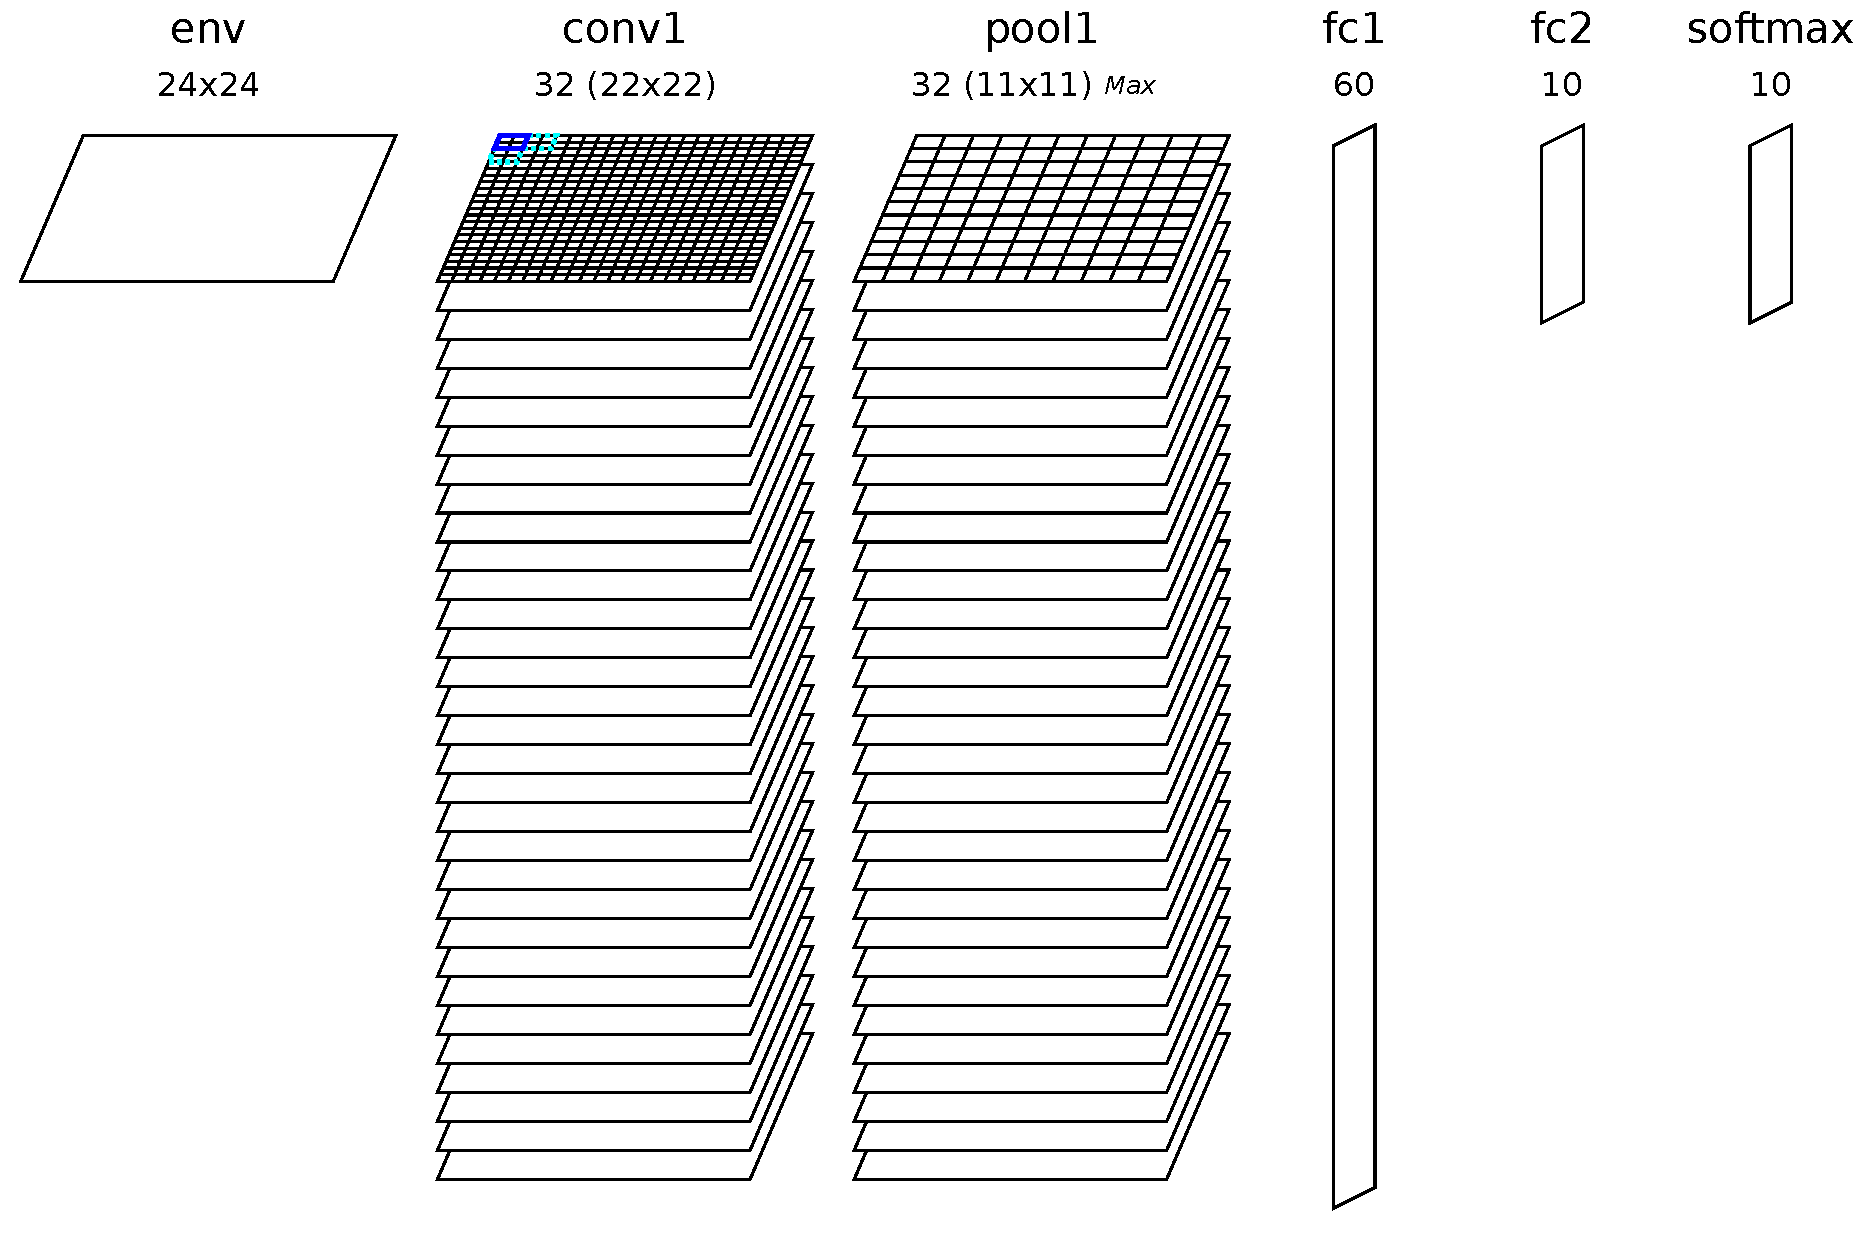
\includegraphics[width=0.75\linewidth]{figs/dnn_example.pdf}
  \caption{Automatically generated and ready to learn DNN from the INI
  configuration file example.}
  \label{fig:DNNExample}
\end{figure}

The learning is accelerated in GPU using the NVIDIA\textregistered{} cuDNN
framework, integrated into the toolflow. Using GPU acceleration, learning times
 can be reduced typically by two orders of magnitude, enabling the learning of
  large databases within tens of minutes to a few hours instead of several days
   or weeks for non-GPU accelerated learning.


\subsection{Performances evaluation}

The software automatically outputs all the information needed for the network
 applicative performances analysis, such as the recognition rate and the
 validation score during the learning; the confusion matrix during learning,
  validation and test; the memory and computation requirements of the network;
  the output maps activity for each layer, and so on, as shown in figure
   \ref{fig:metrics}.

\begin{figure}[!htb]
    \centering
    \begin{tabular}{cc}
    \subf{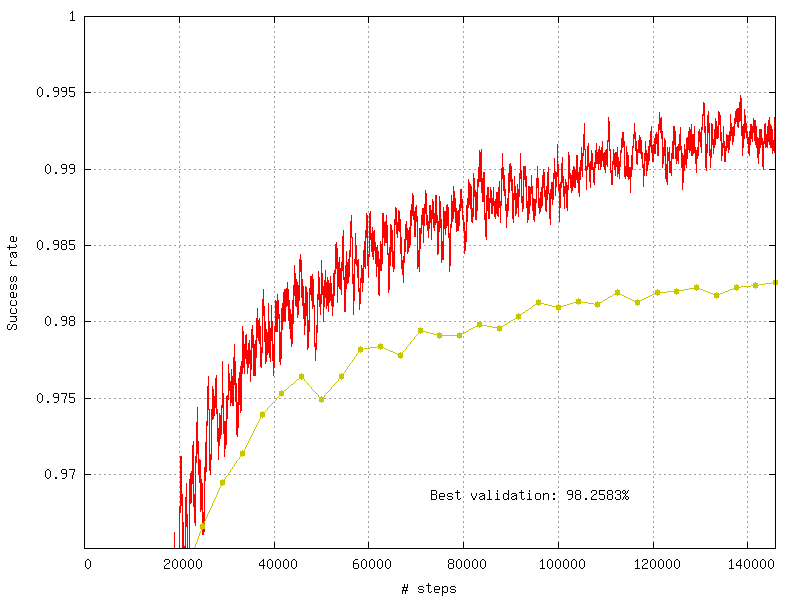
\includegraphics[width=0.45\linewidth,height=0.5\linewidth,
    keepaspectratio]{figs/validation_score.png}}
         {Recognition rate and validation score}
    &
    \subf{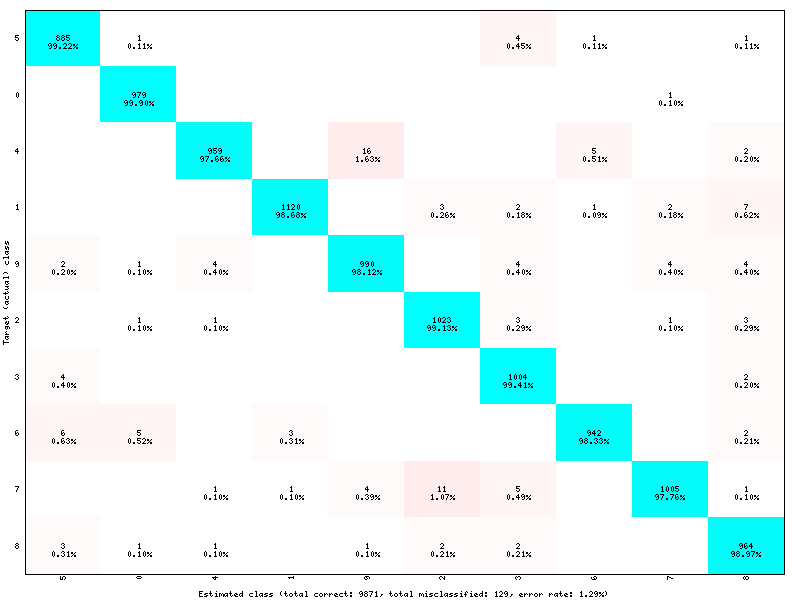
\includegraphics[width=0.45\linewidth,height=0.5\linewidth,
    keepaspectratio]{figs/confusion_matrix.png}}
         {Confusion matrix}
    \\
    \subf{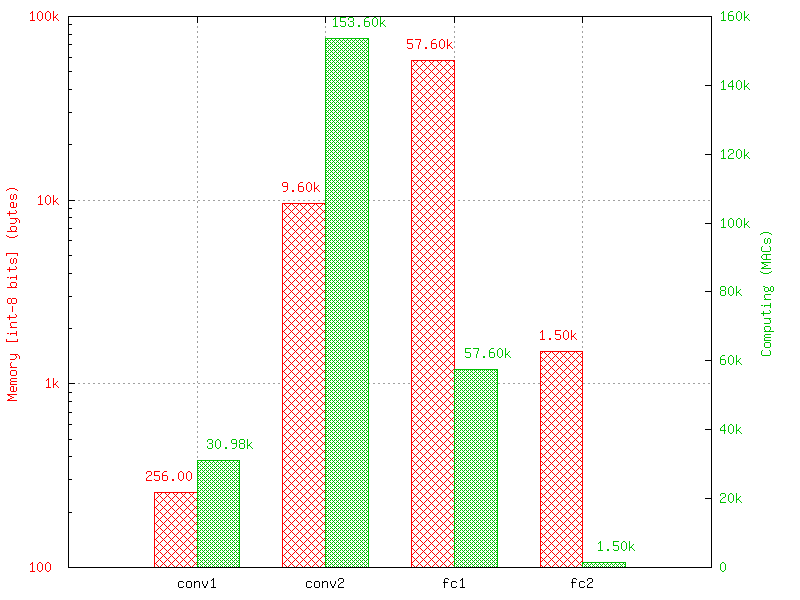
\includegraphics[width=0.45\linewidth,height=0.5\linewidth,
    keepaspectratio]{figs/stats.png}}
         {Memory and computation requirements}
    &
    \subf{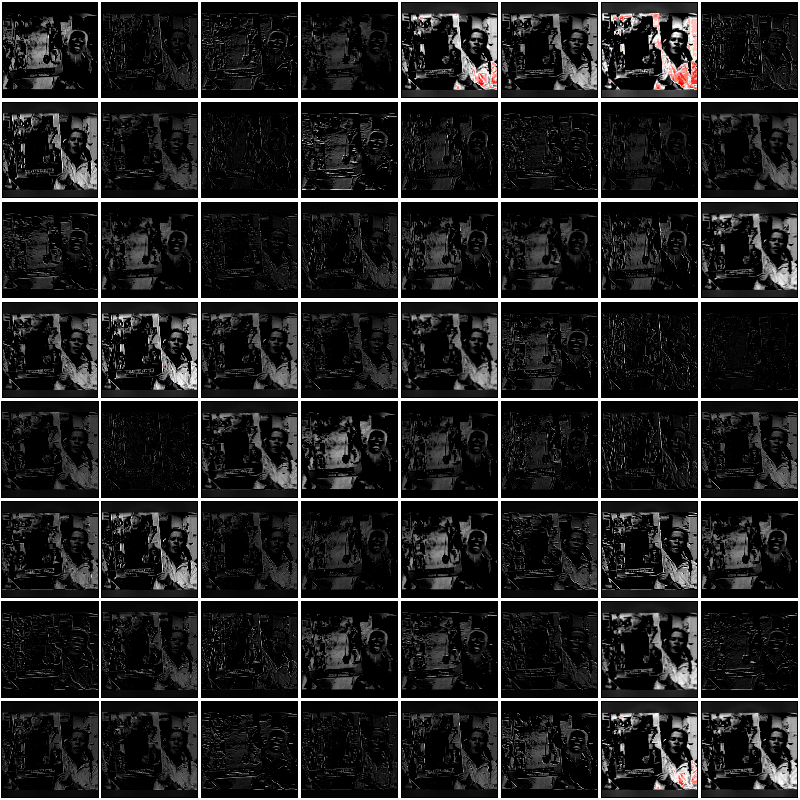
\includegraphics[width=0.38\linewidth,height=0.35\linewidth,
    keepaspectratio]{figs/conv1-dat.png}}
         {Output maps activity}
    \\
    \end{tabular}
  \caption{Example of information automatically generated by the software
  during and after learning.}
  \label{fig:metrics}
\end{figure}


\subsection{Hardware exports}

Once the learned DNN recognition rate performances are satisfying, an optimized
version of the network can be automatically exported for various embedded
targets. An automated network computation performances benchmarking can also
 be performed among different targets.

The following targets are currently supported by the toolflow:
\begin{myitemize}
    \item Plain C code (no dynamic memory allocation, no floating
    point processing);
    \item C code accelerated with OpenMP;
    \item C code tailored for High-Level Synthesis (HLS) with
    Xilinx\textregistered{} Vivado\textregistered{} HLS;
    \subitem Direct synthesis to FPGA, with timing and utilization after
     routing;
    \subitem Possibility to constrain the maximum number of clock cycles desired
     to compute the whole network;
    \subitem FPGA utilization vs number of clock cycle trade-off analysis;
    \item OpenCL code optimized for either CPU/DSP or GPU;
    \item Cuda kernels, cuDNN and TensorRT code optimized for NVIDIA\textregistered{}
    GPUs.
\end{myitemize}

Different automated optimizations are embedded in the exports:
\begin{myitemize}
    \item DNN weights and signal data precision reduction (down to 8 bit
    integers or less for custom FPGA IPs);
    \item Non-linear network activation functions approximations;
    %\item Sparse weights storage when the percentage of weights close to
    % 0 is high;
    \item Different weights discretization methods.
\end{myitemize}

The exports are generated automatically and come with a Makefile and a working
 testbench, including the pre-processed testing dataset.
Once generated, the testbench is ready to be compiled and executed on the target
 platform. The applicative performance (recognition rate) as well as the
 computing time per input data can then be directly mesured by the testbench.

\begin{figure}[!htb]
  \centering
  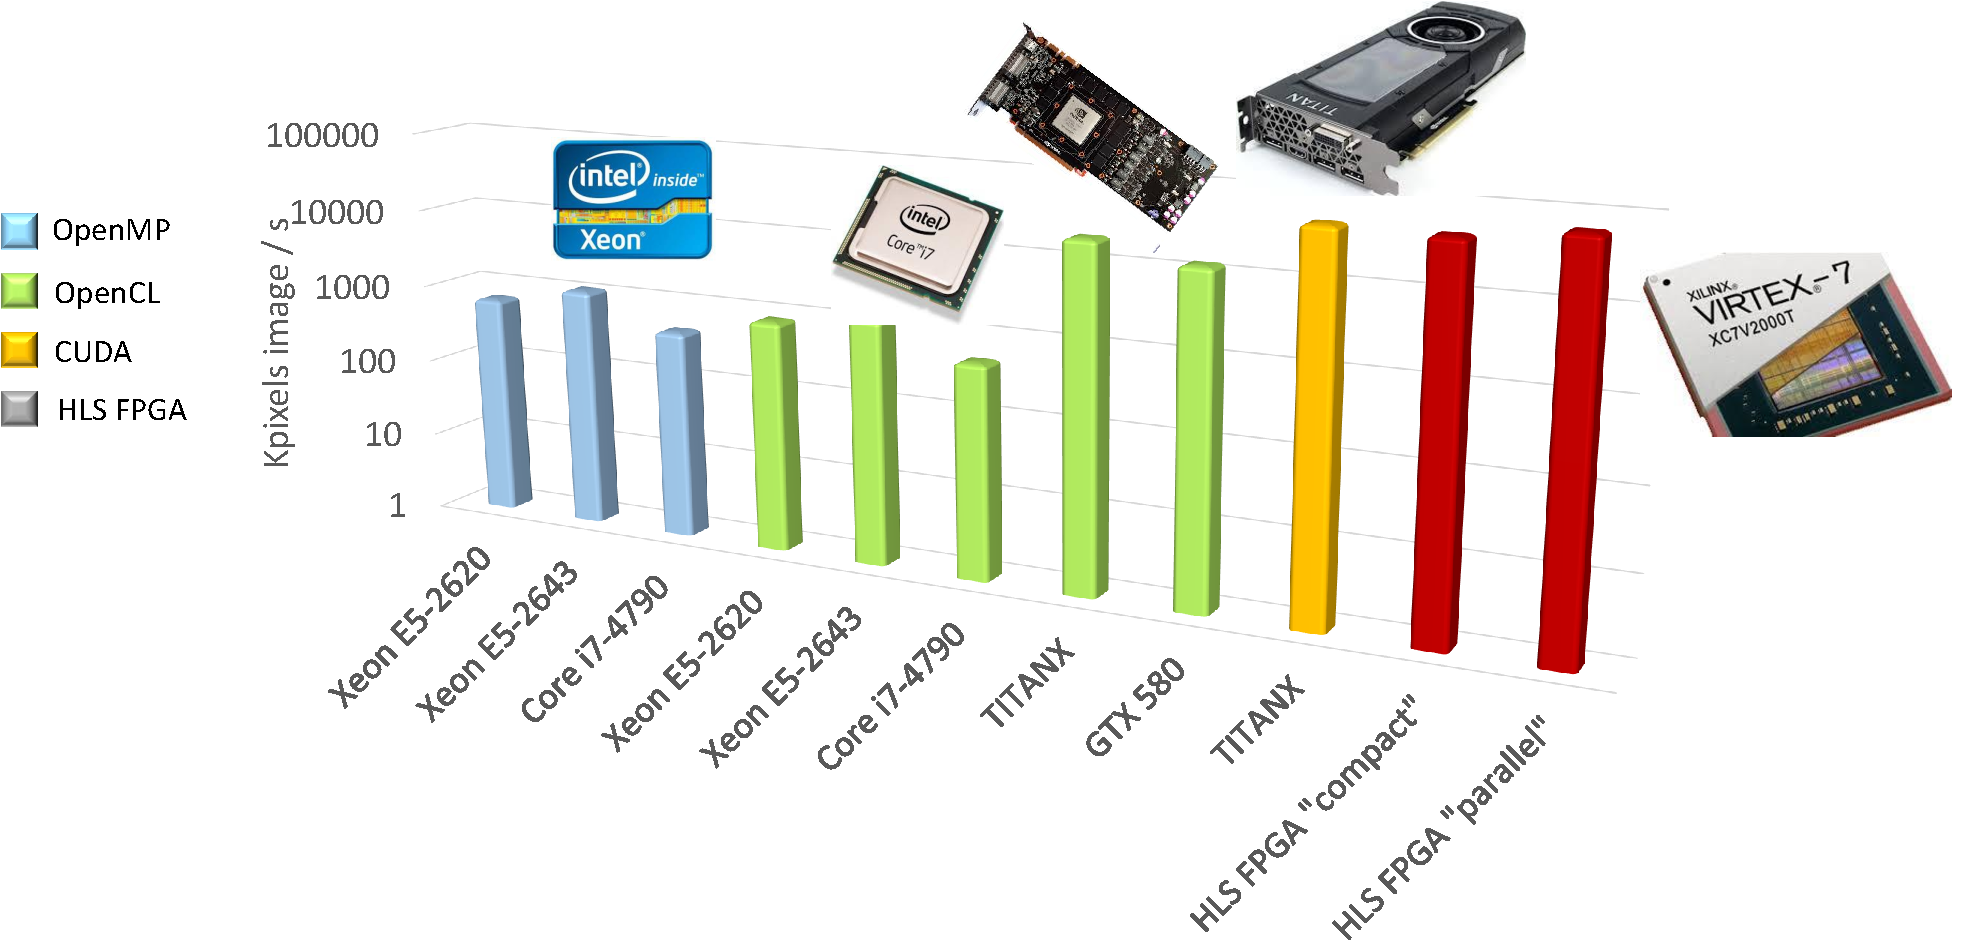
\includegraphics[width=0.95\linewidth]{figs/targets_benchmarking.pdf}
  \caption{Example of network benchmarking on different hardware targets.}
  \label{fig:TargetsBenchmarking}
\end{figure}

The figure \ref{fig:TargetsBenchmarking} shows an example of benchmarking
results of the previous DNN on different targets (in log scale).
Compared to desktop CPUs, the number of input image pixels processed per second
 is more than one order of magnitude higher with GPUsand at least two orders
 of magnitude better with synthesized DNN on FPGA.

\subsection{Summary}

The N2D2 platform is today a complete and production ready neural network
building tool, which does not require advanced knownledges in deep learning to
be used. It is tailored for fast neural network applications generation and
porting with minimum overhead in terms of database creation and management,
data pre-processing, networks configuration and optimized code generation,
which can save months of manual porting and verification effort to a single
automated step in the tool.


\clearpage


\iffullmanual

\clearpage
\section{\label{sec:N2D2-IP}About N2D2-IP}

While N2D2 is our deep learning open-source core framework, some modules referred as "N2D2-IP" in the manual, are only available through custom license agreement with CEA LIST.

If you are interested in obtaining some of these modules, please contact our business developer for more information on available licensing options:

\begin{quote}
Sandrine VARENNE (\href{mailto:Sandrine.VARENNE@cea.fr?subject=[N2D2-IP inquiry]&body=I am interested in obtaining [...] N2D2-IP module(s).\%0A\%0A[please describe briefly the intended usage].\%0A\%0A[your affiliation and contact information].}{Sandrine.VARENNE@cea.fr})
\end{quote}

In addition to N2D2-IP modules, we can also provide our expertise to design specific solutions for integrating DNN in embedded hardware systems, where power, latency, form factor and/or cost are constrained. We can target CPU/DSP/GPU CoTS hardware as well as our own PNeuro (programmable) and DNeuro (dataflow) dedicated hardware accelerator IPs for DNN on FPGA or ASIC.

\section{Performing simulations}

\subsection{Obtaining the latest version of this manual}

Before going further, please make sure you are reading the latest version of
 this manual.
It is located in the {\tt{}manual} sub-directory. To compile the manual
in PDF, just run
the following command:
\begin{lstlisting}
cd manual && make
\end{lstlisting}

In order to compile the manual, you must have \lstinline!pdflatex! and \lstinline!bibtex! installed, as well as some common LaTeX packages.

\begin{myitemize}
    \item On Ubuntu, this can be done by installing the \lstinline!texlive! and \lstinline!texlive-latex-extra! software packages.
    \item On Windows, you can install the \lstinline!MiKTeX! software, which includes everything needed and will install the required LaTeX packages on the fly.
\end{myitemize}


\subsection{Minimum system requirements}

\begin{myitemize}
    \item Supported processors:
        \subitem ARM Cortex A15 (tested on Tegra K1)
        \subitem ARM Cortex A53/A57 (tested on Tegra X1)
        \subitem Pentium-compatible PC (Pentium III, Athlon or more-recent system recommended)
    \item Supported operating systems:
        \subitem Windows $\geq$ 7 or Windows Server $\geq$ 2012, 64 bits with Visual Studio $\geq$ 12 (2013)
        \subitem GNU/Linux with GCC $\geq$ 4.4 (tested on RHEL $\geq$ 6, Debian $\geq$ 6, Ubuntu $\geq$ 14.04)
    \item At least 256 MB of RAM (1 GB with GPU/CUDA) for MNIST dataset processing
    \item At least 150 MB available hard disk space + 350 MB for MNIST dataset processing
\end{myitemize}

For CUDA acceleration:

\begin{myitemize}
    \item CUDA $\geq$ 6.5 and CuDNN $\geq$ 1.0
    \item NVIDIA GPU with CUDA compute capability $\geq$ 3 (starting from \emph{Kepler} micro-architecture)
    \item At least 512 MB GPU RAM for MNIST dataset processing
\end{myitemize}


\subsection{Obtaining N2D2}

\subsubsection{Prerequisites}

\paragraph{Red Hat Enterprise Linux (RHEL) 6}

Make sure you have the following packages installed:
\begin{myitemize}
    \item \lstinline!cmake!
    \item \lstinline!gnuplot!
    \item \lstinline!opencv!
    \item \lstinline!opencv-devel! (may require the
    \lstinline!rhel-x86_64-workstation-optional-6! repository channel)
\end{myitemize}

Plus, to be able to use GPU acceleration:
\begin{myitemize}
    \item Install the CUDA repository package:
\begin{lstlisting}
rpm -Uhv http://developer.download.nvidia.com/compute/cuda/repos/rhel6/x86_64/cuda-repo-rhel6-7.5-18.x86_64.rpm
yum clean expire-cache
yum install cuda
\end{lstlisting}
    \item Install cuDNN from the NVIDIA website: register to
    \href{https://developer.nvidia.com/cudnn}{NVIDIA Developer} and download
    the latest version of cuDNN.
    Simply copy the header and library files from the cuDNN archive to the
    corresponding directories in the CUDA installation path (by default:
     {\tt{}/usr/local/cuda/include} and {\tt{}/usr/local/cuda/lib64},
     respectively).
    \item Make sure the CUDA library path (e.g. {\tt{}/usr/local/cuda/lib64}) is
     added to the {\tt{}LD\_LIBRARY\_PATH} environment variable.
\end{myitemize}

\paragraph{Ubuntu}

Make sure you have the following packages installed, if they are available on
your Ubuntu version:
\begin{myitemize}
    \item \lstinline!cmake!
    \item \lstinline!gnuplot!
    \item \lstinline!libopencv-dev!
    \item \lstinline!libcv-dev!
    \item \lstinline!libhighgui-dev!
\end{myitemize}

Plus, to be able to use GPU acceleration:
\begin{myitemize}
    \item Install the CUDA repository package matching your distribution. For
    example, for Ubuntu 14.04 64 bits:
\begin{lstlisting}[escapechar=!]
wget http://developer.download.nvidia.com/compute/cuda/repos/ubuntu!\color{gray}{1404}!/!\color{gray}{x86\_64}!/cuda-repo-ubuntu!\color{gray}{1404}!_7.5-18_!\color{gray}{amd64}!.deb
dpkg -i cuda-repo-ubuntu!\color{gray}{1404}!_7.5-18_!\color{gray}{amd64}!.deb
\end{lstlisting}
    \item Install the cuDNN repository package matching your distribution. For
    example, for Ubuntu 14.04 64 bits:
\begin{lstlisting}[escapechar=!]
wget http://developer.download.nvidia.com/compute/machine-learning/repos/ubuntu!\color{gray}{1404}!/!\color{gray}{x86\_64}!/nvidia-machine-learning-repo-ubuntu!\color{gray}{1404}!_4.0-2_!\color{gray}{amd64}!.deb
dpkg -i nvidia-machine-learning-repo-ubuntu!\color{gray}{1404}!_4.0-2_!\color{gray}{amd64}!.deb
\end{lstlisting}
    Note that the cuDNN repository package is provided by NVIDIA for Ubuntu starting
    from version 14.04.
    \item Update the package lists: \lstinline!apt-get update!
    \item Install the CUDA and cuDNN required packages:
\begin{lstlisting}[escapechar=!]
apt-get install cuda-core-7-5 cuda-cudart-dev-7-5 cuda-cublas-dev-7-5 cuda-curand-dev-7-5 libcudnn5-dev
\end{lstlisting}
    \item Make sure there is a symlink to \lstinline!/usr/local/cuda!:
\begin{lstlisting}[escapechar=!]
ln -s /usr/local/cuda-7.5 /usr/local/cuda
\end{lstlisting}
    \item Make sure the CUDA library path (e.g. {\tt{}/usr/local/cuda/lib64}) is
     added to the {\tt{}LD\_LIBRARY\_PATH} environment variable.
\end{myitemize}

\paragraph{Windows}

On Windows 64 bits, Visual Studio $\geq$ 12 (2013) is required.

Make sure you have the following software installed:
\begin{myitemize}
    \item CMake (\url{http://www.cmake.org/}): download and run the Windows installer.
    \item \lstinline!dirent.h! C++ header (\url{https://github.com/tronkko/dirent}): to be put in the Visual Studio
    include path.
    \item Gnuplot (\url{http://www.gnuplot.info/}): the bin sub-directory in
    the install path needs to be added to the Windows \lstinline!PATH!
     environment variable.
    \item OpenCV (\url{http://opencv.org/}): download the latest 2.x version
    for Windows and extract it to, for example,
    \lstinline!C:\OpenCV\!.
  Make sure to define the environment variable \lstinline!OpenCV_DIR! to point
  to \lstinline!C:\OpenCV\opencv\build!.
  Make sure to add the bin sub-directory (%%
\lstinline!C:\OpenCV\opencv\build\x64\vc12\bin!) to the Windows
  \lstinline!PATH! environment variable.
\end{myitemize}

Plus, to be able to use GPU acceleration:
\begin{myitemize}
    \item Download and install CUDA toolkit 8.0 located at \url{https://developer.nvidia.com/compute/cuda/8.0/prod/local_installers/cuda_8.0.44_windows-exe}:
\begin{lstlisting}[escapechar=!]
rename cuda_8.0.44_windows-exe cuda_8.0.44_windows.exe
cuda_8.0.44_windows.exe -s compiler_8.0 cublas_8.0 cublas_dev_8.0 cudart_8.0 curand_8.0 curand_dev_8.0
\end{lstlisting}
    \item Update the \lstinline!PATH! environment variable:
\begin{lstlisting}[escapechar=!]
set PATH=%ProgramFiles%\NVIDIA GPU Computing Toolkit\CUDA\v8.0\bin;%ProgramFiles%\NVIDIA GPU Computing Toolkit\CUDA\v8.0\libnvvp;%PATH%
\end{lstlisting}
    \item Download and install cuDNN 8.0 located at \url{http://developer.download.nvidia.com/compute/redist/cudnn/v5.1/cudnn-8.0-windows7-x64-v5.1.zip} (the following command assumes that you have 7-Zip installed):
\begin{lstlisting}[escapechar=!]
7z x cudnn-8.0-windows7-x64-v5.1.zip
copy cuda\include\*.* ^
  "%ProgramFiles%\NVIDIA GPU Computing Toolkit\CUDA\v8.0\include\"
copy cuda\lib\x64\*.* ^
  "%ProgramFiles%\NVIDIA GPU Computing Toolkit\CUDA\v8.0\lib\x64\"
copy cuda\bin\*.* ^
  "%ProgramFiles%\NVIDIA GPU Computing Toolkit\CUDA\v8.0\bin\"
\end{lstlisting}
\end{myitemize}


\subsubsection{Getting the sources}

\noindent Use the following command:
\begin{lstlisting}
git clone git@github.com:CEA-LIST/N2D2.git
\end{lstlisting}

\subsubsection{Compilation}

\noindent To compile the program:
\begin{lstlisting}
mkdir build
cd build
cmake .. && make
\end{lstlisting}

On Windows, you may have to specify the generator, for example:
\begin{lstlisting}
cmake .. -G"Visual Studio 12"
\end{lstlisting}

Then open the newly created N2D2 project in Visual Studio 12 (2013). Select
"Release" for the build target. Right click on \lstinline!ALL_BUILD! item and
select "Build".


\subsection{Downloading training datasets}

A python script located in the repository root directory allows you to select and
 automatically download some well-known datasets, like MNIST and GTSRB
 (the script requires Python 2.x with bindings for GTK 2 package):
\begin{lstlisting}
./tools/install_stimuli_gui.py
\end{lstlisting}

By default, the datasets are downloaded in the path specified in the
 \lstinline!N2D2_DATA! environment variable, which is the root path used by the
 N2D2 tool to locate the databases. If the \lstinline!N2D2_DATA! variable is
  not set, the default value used is {\tt{}/local/\$USER/n2d2\_data/}
  (or {\tt{}/local/n2d2\_data/} if the \lstinline!USER! environment variable
   is not set) on Linux and {\tt{}C:\textbackslash{}n2d2\_data\textbackslash{}}
    on Windows.

Please make sure you have write access to the \lstinline!N2D2_DATA! path, or if
not set, in the default {\tt{}/local/\$USER/n2d2\_data/} path.


\subsection{Run the learning}

The following command will run the learning for 600,000 image
presentations/steps and log the performances of the network every 10,000 steps:
\begin{lstlisting}
./n2d2 "mnist24_16c4s2_24c5s2_150_10.ini" -learn 600000 -log 10000
\end{lstlisting}

Note: you may want to check the gradient computation using the
 \lstinline!-check! option. Note that it can be extremely long and can
occasionally fail if the required precision is too high.

\subsection{Test a learned network}

After the learning is completed, this command evaluate the network performances
 on the test data set:
\begin{lstlisting}
./n2d2 "mnist24_16c4s2_24c5s2_150_10.ini" -test
\end{lstlisting}


\subsubsection{Interpreting the results}

\paragraph{Recognition rate}

The recognition rate and the validation score are reported during the learning
 in the \emph{TargetScore\_*/Success\_validation.png} file, as shown in
 figure \ref{fig:validationScore}.

\begin{figure}[!htb]
  \centering
  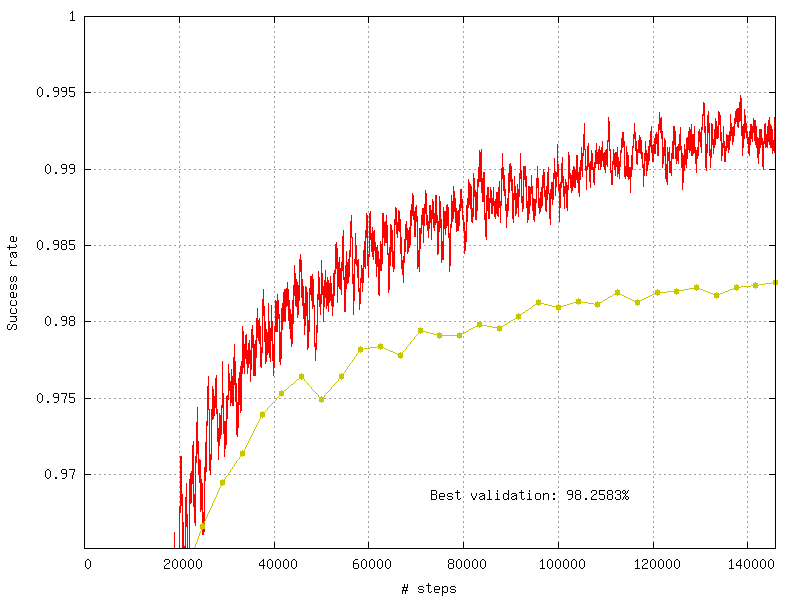
\includegraphics[width=0.8\linewidth]{figs/validation_score.png}
  \caption{Recognition rate and validation score during learning.}
  \label{fig:validationScore}
\end{figure}

\paragraph{Confusion matrix}

The software automatically outputs the confusion matrix during learning,
validation and test, with an example shown in figure \ref{fig:ConfusionMatrix}.
Each row of the matrix contains the number of occurrences estimated by the
 network for each label, for all the data corresponding to a single actual,
 target label.
Or equivalently, each column of the matrix contains the number of actual,
target label occurrences, corresponding to the same estimated label.
Idealy, the matrix should be diagonal, with no occurrence of an estimated
 label for a different actual label (network mistake).

\begin{figure}[!htb]
  \centering
  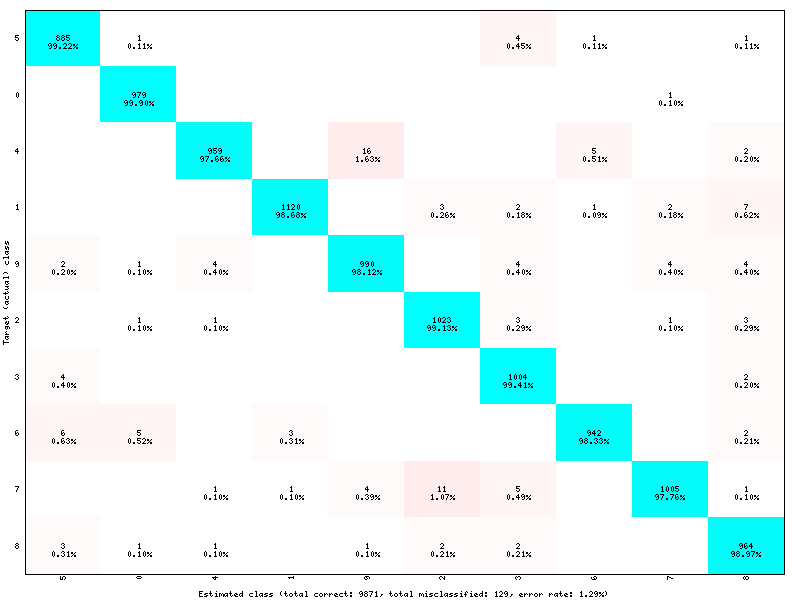
\includegraphics[width=0.8\linewidth]{figs/confusion_matrix.png}
  \caption{Example of confusion matrix obtained after the learning.}
  \label{fig:ConfusionMatrix}
\end{figure}

The confusion matrix reports can be found in the simulation directory:
\begin{myitemize}
\item \emph{TargetScore\_*/ConfusionMatrix\_learning.png};
\item \emph{TargetScore\_*/ConfusionMatrix\_validation.png};
\item \emph{TargetScore\_*/ConfusionMatrix\_test.png}.
\end{myitemize}

\paragraph{Memory and computation requirements}

The software also report the memory and computation requirements of the network,
 as shown in figure \ref{fig:stats}. The corresponding report can be found in
 the \emph{stats} sub-directory of the simulation.

\begin{figure}[!htb]
  \centering
  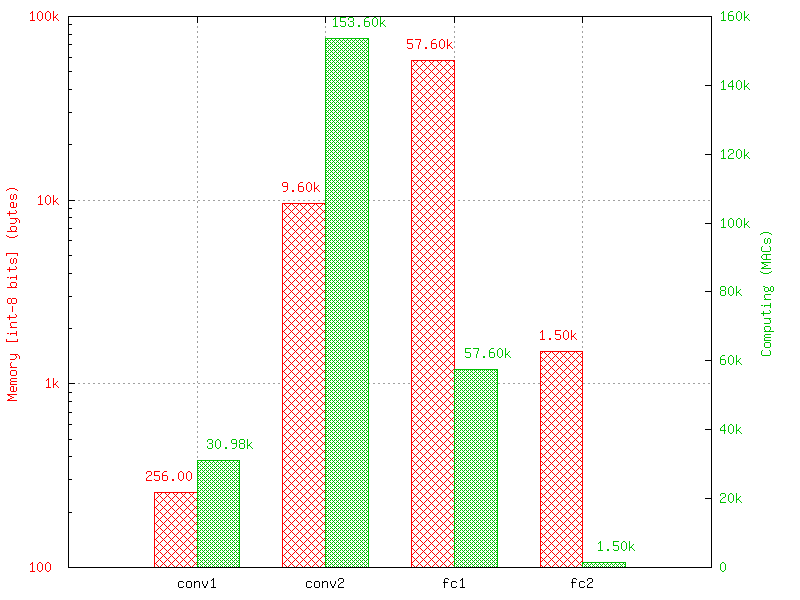
\includegraphics[width=0.8\linewidth]{figs/stats.png}
  \caption{Example of memory and computation requirements of the network.}
  \label{fig:stats}
\end{figure}


\paragraph{Kernels and weights distribution}

The synaptic weights obtained during and after the learning can be analyzed,
in terms of distribution (\emph{weights} sub-directory of the simulation) or in
terms of kernels (\emph{kernels} sub-directory of the simulation), as shown
in \ref{fig:weights}.


\begin{figure}[!htb]
    \centering
    \begin{tabular}{cc}
    \subf{\includegraphics[width=0.48\linewidth,height=0.5\linewidth,
    keepaspectratio]{figs/conv1.png}}
         {\emph{conv1} kernels}
    &
    \subf{\includegraphics[width=0.48\linewidth,height=0.5\linewidth,
    keepaspectratio]{figs/conv2.png}}
         {\emph{conv2} kernels}
    \\
    \subf{\includegraphics[width=0.48\linewidth,height=0.5\linewidth,
    keepaspectratio]{figs/conv1-distrib.png}}
         {\emph{conv1} weights distribution}
    &
    \subf{\includegraphics[width=0.48\linewidth,height=0.5\linewidth,
    keepaspectratio]{figs/conv2-distrib.png}}
         {\emph{conv2} weights distribution}
    \\
    \end{tabular}
  \caption{Example of kernels and weights distribution analysis for two
   convolutional layers.}
  \label{fig:weights}
\end{figure}


\paragraph{Output maps activity}

The initial output maps activity for each layer can be visualized in the
 \emph{outputs\_init} sub-directory of the simulation, as shown in figure
  \ref{fig:outputs}.

\begin{figure}[!htb]
  \centering
  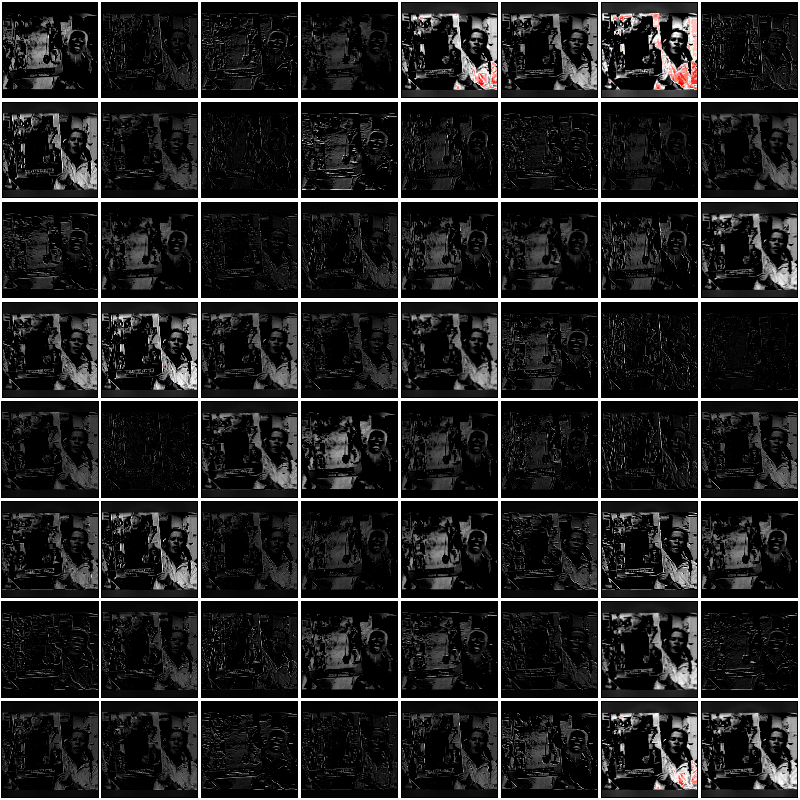
\includegraphics[width=0.6\linewidth]{figs/conv1-dat.png}
  \caption{Output maps activity example of the first convolutional layer of
  the network.}
  \label{fig:outputs}
\end{figure}



\subsection{Export a learned network}


\begin{lstlisting}
./n2d2 "mnist24_16c4s2_24c5s2_150_10.ini" -export CPP_OpenCL
\end{lstlisting}

Export types:
\begin{myitemize}
\item \lstinline!C! C export using OpenMP;
\item \lstinline!C_HLS! C export tailored for HLS with Vivado HLS;
\item \lstinline!CPP_OpenCL! C++ export using OpenCL;
\item \lstinline!CPP_Cuda! C++ export using Cuda;
\item \lstinline!CPP_cuDNN! C++ export using cuDNN;
\item \lstinline!CPP_TensorRT! C++ export using tensorRT 2.1 API;
\item \lstinline!SC_Spike! SystemC spike export.
\end{myitemize}

Other program options related to the exports:
\begin{center}
 \begin{tabular}{| p{5cm} | p{10cm} | }
 \hline
 Option [default value] & Description\\
 \hline\hline
  \lstinline!-uenv! & If present, treat the input stimuli data as unsigned \\
  \lstinline!-nbbits! [8] & Number of bits for the weights and signals.
  Must be 8, 16, 32 or 64 for integer export, or -32, -64 for floating
  point export. The number of bits can be arbitrary for the \lstinline!C_HLS!
  export (for example, 6 bits) \\
 \hline
\end{tabular}
\end{center}


\subsubsection{\texorpdfstring{%%
\lstinline[basicstyle=\ttfamily\bfseries]!C! export\protect\iponly}{C export}}

Test the exported network:
\begin{lstlisting}
cd export_C_int8
make
./bin/n2d2_test
\end{lstlisting}

The result should look like:
\begin{lstlisting}[style=console]
...
1652.00/1762    (avg = 93.757094%)
1653.00/1763    (avg = 93.760635%)
1654.00/1764    (avg = 93.764172%)
Tested 1764 stimuli
Success rate = 93.764172%
Process time per stimulus = 187.548186 us (12 threads)

Confusion matrix:
-------------------------------------------------
| T \ E |       0 |       1 |       2 |       3 |
-------------------------------------------------
|     0 |     329 |       1 |       5 |       2 |
|       |  97.63% |   0.30% |   1.48% |   0.59% |
|     1 |       0 |     692 |       2 |       6 |
|       |   0.00% |  98.86% |   0.29% |   0.86% |
|     2 |      11 |      27 |     609 |      55 |
|       |   1.57% |   3.85% |  86.75% |   7.83% |
|     3 |       0 |       0 |       1 |      24 |
|       |   0.00% |   0.00% |   4.00% |  96.00% |
-------------------------------------------------
T: Target    E: Estimated
\end{lstlisting}

\subsubsection{\texorpdfstring{%%
\lstinline[basicstyle=\ttfamily\bfseries]!CPP_OpenCL! export\protect\iponly}
{CPP\_OpenCL export}}
The OpenCL export can run the generated program in GPU or CPU architectures.
Compilation features:
\begin{center}
 \begin{tabular}{| p{7cm} | p{8cm} | }
 \hline
 Preprocessor command [default value] & Description\\
 \hline\hline
  \lstinline!PROFILING! [0] & Compile the binary with a synchronization between
   each layers and return the mean execution time of each layer.
  This preprocessor option can decrease performances.\\
  \lstinline!GENERATE_KBIN! [0] & Generate the binary output of the OpenCL
  kernel .cl file use. The binary is store in the /bin folder. \\
  \lstinline!LOAD_KBIN! [0] & Indicate to the program to load an OpenCL
  kernel as a binary from the /bin folder instead of a .cl file. \\
  \lstinline!CUDA! [0] & Use the CUDA OpenCL SDK locate at
  ${/usr/local/cuda}$ \\
  \lstinline!MALI! [0] & Use the MALI OpenCL SDK locate at
  ${/usr/Mali_OpenCL_SDK_vXXX}$ \\
  \lstinline!INTEL! [0] & Use the INTEL OpenCL SDK locate at
  ${/opt/intel/opencl}$ \\
  \lstinline!AMD! [1] & Use the AMD OpenCL SDK locate at
  ${/opt/AMDAPPSDK-XXX}$ \\
 \hline
\end{tabular}
\end{center}

Program options related to the OpenCL export:
\begin{center}
 \begin{tabular}{| p{5cm} | p{10cm} | }
 \hline
 Option [default value] & Description\\
 \hline\hline
  \lstinline!-cpu! & If present, force to use a CPU architecture to run
  the program \\
  \lstinline!-gpu! & If present, force to use a GPU architecture to run
  the program \\
  \lstinline!-batch! [1] & Size of the batch to use \\
  \lstinline!-stimulus! [NULL] & Path to a specific input stimulus to test.
  For example: -stimulus ${/stimulus/env0000.pgm}$ command will test the file
  env0000.pgm  of the stimulus folder.\\
 \hline
\end{tabular}
\end{center}

Test the exported network:
\begin{lstlisting}
cd export_CPP_OpenCL_float32
make
./bin/n2d2_opencl_test -gpu
\end{lstlisting}

\subsubsection{\texorpdfstring{%%
\lstinline[basicstyle=\ttfamily\bfseries]!CPP_TensorRT! export}{CPP\_TensorRT export}}
The tensorRT 2.1 API export can run the generated program in NVIDIA GPU architecture.
It use CUDA and tensorRT 2.1 API library.
The currently supported layers by the tensorRT 2.1 export are : Convolutional, Pooling, Concatenation,
Fully-Connected, Softmax and all activations type.
Custom layers implementation through the plugin factory and
 generic 8-bits calibrations inference features are under development.

Program options related to the tensorRT 2.1 API export:
\begin{center}
 \begin{tabular}{| p{5cm} | p{10cm} | }
 \hline
 Option [default value] & Description\\
 \hline\hline
  \lstinline!-batch! [1] & Size of the batch to use \\
  \lstinline!-dev! [0] & CUDA Device ID selection  \\
  \lstinline!-stimulus! [NULL] & Path to a specific input stimulus to test.
  For example: -stimulus ${/stimulus/env0000.pgm}$ command will test the file
   env0000.pgm  of the stimulus folder.\\
  \lstinline!-prof! & Activates the layer wise profiling mechanism. This option
  can decrease execution time performance.\\
  \lstinline!-iter-build! [1] & Sets the number of minimization build iterations
  done by the tensorRT builder to find the best layer tactics.\\
 \hline
\end{tabular}
\end{center}

Test the exported network with layer wise profiling:
\begin{lstlisting}
cd export_CPP_TensorRT_float32
make
./bin/n2d2_tensorRT_test -prof
\end{lstlisting}

The results of the layer wise profiling should look like:
\begin{lstlisting}[style=console]
(19%)  **************************************** CONV1 + CONV1_ACTIVATION: 0.0219467 ms
(05%)  ************ POOL1: 0.00675573 ms
(13%)  **************************** CONV2 + CONV2_ACTIVATION: 0.0159089 ms
(05%)  ************ POOL2: 0.00616047 ms
(14%)  ****************************** CONV3 + CONV3_ACTIVATION: 0.0159713 ms
(19%)  **************************************** FC1 + FC1_ACTIVATION: 0.0222242 ms
(13%)  **************************** FC2: 0.0149013 ms
(08%)  ****************** SOFTMAX: 0.0100633 ms
Average profiled tensorRT process time per stimulus = 0.113932 ms

\end{lstlisting}

\subsubsection{\texorpdfstring{%%
\lstinline[basicstyle=\ttfamily\bfseries]!CPP_cuDNN! export}{CPP\_cuDNN export}}
The cuDNN export can run the generated program in NVIDIA GPU architecture.
It use CUDA and cuDNN library.
Compilation features:
\begin{center}
 \begin{tabular}{| p{7cm} | p{8cm} | }
 \hline
 Preprocessor command [default value] & Description\\
 \hline\hline
  \lstinline!PROFILING! [0] & Compile the binary with a synchronization
  between each layers and return the mean execution time of each layer.
  This preprocessor option can decrease performances.\\
  \lstinline!ARCH32! [0] & Compile the binary with the 32-bits architecture
   compatibility.\\
 \hline
\end{tabular}
\end{center}

Program options related to the cuDNN export:
\begin{center}
 \begin{tabular}{| p{5cm} | p{10cm} | }
 \hline
 Option [default value] & Description\\
 \hline\hline
  \lstinline!-batch! [1] & Size of the batch to use \\
  \lstinline!-dev! [0] & CUDA Device ID selection  \\
  \lstinline!-stimulus! [NULL] & Path to a specific input stimulus to test.
  For example: -stimulus ${/stimulus/env0000.pgm}$ command will test the file
   env0000.pgm  of the stimulus folder.\\
 \hline
\end{tabular}
\end{center}

Test the exported network:
\begin{lstlisting}
cd export_CPP_cuDNN_float32
make
./bin/n2d2_cudnn_test
\end{lstlisting}

\subsubsection{\texorpdfstring{%%
\lstinline[basicstyle=\ttfamily\bfseries]!C_HLS! export\protect\iponly}
{C\_HLS export}}

Test the exported network:
\begin{lstlisting}
cd export_C_HLS_int8
make
./bin/n2d2_test
\end{lstlisting}

Run the High-Level Synthesis (HLS) with Xilinx\textregistered{}
Vivado\textregistered{} HLS:
\begin{lstlisting}
vivado_hls -f run_hls.tcl
\end{lstlisting}

\clearpage

\section{INI file interface}

The INI file interface is the primary way of using N2D2. It is a simple,
lightweight and user-friendly format for specifying a complete DNN-based
application, including dataset instanciation, data pre-processing, neural
network layers instanciation and post-processing, with all its hyperparameters.

\subsection{Syntax}

INI files are simple text files with a basic structure composed of sections,
properties and values.

\subsubsection{Properties}

The basic element contained in an INI file is the property. Every property has
a name and a value, delimited by an equals sign (=). The name appears to the
left of the equals sign.

\begin{lstlisting}[language=ini]
name=value
\end{lstlisting}

\subsubsection{Sections}

Properties may be grouped into arbitrarily named sections. The section name
appears on a line by itself, in square brackets ([ and ]). All properties after
the section declaration are associated with that section. There is no explicit
"end of section" delimiter; sections end at the next section declaration, or the
end of the file. Sections may not be nested.

\begin{lstlisting}[language=ini]
[section]
a=a
b=b
\end{lstlisting}

\subsubsection{Case sensitivity}

Section and property names are case sensitive.

\subsubsection{Comments}

Semicolons (\lstinline!;!) or number sign (\lstinline!#!) at the beginning or in
 the middle of the line indicate a comment. Comments are ignored.

\begin{lstlisting}[language=ini]
; comment text
a=a # comment text
a="a ; not a comment" ; comment text
\end{lstlisting}

\subsubsection{Quoted values}

Values can be quoted, using double quotes. This allows for explicit declaration
of whitespace, and/or for quoting of special characters (equals, semicolon,
etc.).

\subsubsection{Whitespace}

Leading and trailing whitespace on a line are ignored.

\subsubsection{Escape characters}

A backslash (\lstinline!\!) followed immediately by EOL (end-of-line) causes the
 line break to be ignored.

\subsection{Template inclusion syntax}

Is is possible to recursively include templated INI files. For example, the main
INI file can include a templated file like the following:

\begin{lstlisting}[language=ini]
[inception@inception_model.ini.tpl]
INPUT=layer_x
SIZE=32
ARRAY=2 ; Must be the number of elements in the array
ARRAY[0].P1=Conv
ARRAY[0].P2=32
ARRAY[1].P1=Pool
ARRAY[1].P2=64
\end{lstlisting}

If the \lstinline!inception_model.ini.tpl! template file content is:

\begin{lstlisting}[language=tpl]
[{{SECTION_NAME}}_layer1]
Input={{INPUT}}
Type=Conv
NbChannels={{SIZE}}

[{{SECTION_NAME}}_layer2]
Input={{SECTION_NAME}}_layer1
Type=Fc
NbOutputs={{SIZE}}


[{{SECTION_NAME}}_array{{#}}]
Prop1=Config{{.P1}}
Prop2={{.P2}}

\end{lstlisting}

The resulting equivalent content for the main INI file will be:

\begin{lstlisting}[language=ini]
[inception_layer1]
Input=layer_x
Type=Conv
NbChannels=32

[inception_layer2]
Input=inception_layer1
Type=Fc
NbOutputs=32

[inception_array0]
Prop1=ConfigConv
Prop2=32

[inception_array1]
Prop1=ConfigPool
Prop2=64
\end{lstlisting}

The \lstinline!SECTION_NAME! template parameter is automatically generated from
the name of the including section (before \lstinline!@!).


\subsubsection{Variable substitution}

\lstinline!{{VAR}}! is replaced by the value of the \lstinline!VAR! template
 parameter.


\subsubsection{Control statements}

Control statements are between \lstinline!{\%! and \lstinline!\%}! delimiters.

\paragraph{block}
\lstinline!{\% block ARRAY \%}! ...
\lstinline!{\% endblock \%}!

The \lstinline!#! template parameter is automatically generated from the
\lstinline!{\% block ... \%}! template control statement and corresponds to the
current item position, starting from 0.

\paragraph{for}
\lstinline!{\% for VAR in range([START, ]END]) \%}! ...
\lstinline!{\% endfor \%}!

If \lstinline!START! is not specified, the loop begins at 0 (first value of
\lstinline!VAR!). The last value of \lstinline!VAR! is \lstinline!END!-1.

\paragraph{if}
\lstinline!{\% if VAR OP [VALUE] \%}! ...
\lstinline![{\% else \%}]! ...
\lstinline!{\% endif \%}!

\lstinline!OP! may be \lstinline!==!, \lstinline?!=?, \lstinline!exists! or \lstinline!not_exists!.

\paragraph{include}
\lstinline!{\% include FILENAME \%}!


\subsection{Global parameters}

\begin{center}
 \begin{tabular}{| p{5cm} | p{10cm} | }
 \hline
 Option [default value] & Description\\
 \hline\hline
  \lstinline!DefaultModel! [\lstinline!Transcode!] & Default layers model.
  Can be \lstinline!Frame!, \lstinline!Frame_CUDA!, \lstinline!Transcode!
  or \lstinline!Spike! \\
  \lstinline!SignalsDiscretization! [0] & Number of levels for signal
  discretization \\
  \lstinline!FreeParametersDiscretization! [0] & Number of levels for weights discretization \\
 \hline
\end{tabular}
\end{center}


\subsection{Databases}

The tool integrates pre-defined modules for several well-known database used
in the deep learning community, such as MNIST, GTSRB, CIFAR10 and so on.
That way, no extra step is necessary to be able to directly build a network
and learn it on these database.

\subsubsection{MNIST}

MNIST \citep{LeCun1998} is already fractionned into a learning set and
a testing set, with:
\begin{myitemize}
\item 60,000 digits in the learning set;
\item 10,000 digits in the testing set.
\end{myitemize}

Example:
\begin{lstlisting}[language=ini]
[database]
Type=MNIST_IDX_Database
Validation=0.2  ; Fraction of learning stimuli used for the validation [default: 0.0]
\end{lstlisting}

\begin{center}
 \begin{tabular}{| p{5cm} | p{10cm} | }
 \hline
 Option [default value] & Description\\
 \hline\hline
  \lstinline!Validation! [0.0] & Fraction of the learning set used for
  validation \\
  \lstinline!DataPath! & Path to the database \\
  \noindent [\lstinline!$N2D2_DATA!/mnist] & \\
 \hline
\end{tabular}
\end{center}

\subsubsection{GTSRB}

GTSRB \citep{Stallkamp2012} is already fractionned into a learning set
and a testing set, with:
\begin{myitemize}
\item 39,209 digits in the learning set;
\item 12,630 digits in the testing set.
\end{myitemize}

Example:
\begin{lstlisting}[language=ini]
[database]
Type=GTSRB_DIR_Database
Validation=0.2  ; Fraction of learning stimuli used for the validation [default: 0.0]
\end{lstlisting}

\begin{center}
 \begin{tabular}{| p{5cm} | p{10cm} | }
 \hline
 Option [default value] & Description\\
 \hline\hline
  \lstinline!Validation! [0.0] & Fraction of the learning set used for
   validation \\
  \lstinline!DataPath! & Path to the database \\
  \noindent [\lstinline!$N2D2_DATA!/GTSRB] & \\
 \hline
\end{tabular}
\end{center}

\subsubsection{Directory}

Hand made database stored in files directories are directly supported with
the \lstinline!DIR_Database! module.
For example, suppose your database is organized as following (in the path
specified in the \lstinline!N2D2_DATA! environment variable):
\begin{myitemize}
\item \lstinline!GST/airplanes!: 800 images
\item \lstinline!GST/car_side!: 123 images
\item \lstinline!GST/Faces!: 435 images
\item \lstinline!GST/Motorbikes!: 798 images
\end{myitemize}

You can then instanciate this database as input of your neural network using
the following parameters:
\begin{lstlisting}[language=ini]
[database]
Type=DIR_Database
DataPath=\${N2D2_DATA}/GST
Learn=0.4 ; 40\% of images of the smallest category = 49 (0.4x123) images for each category will be used for learning
Validation=0.2 ; 20\% of images of the smallest category = 25 (0.2x123) images for each category will be used for validation
; the remaining images will be used for testing
\end{lstlisting}

Each subdirectory will be treated as a different label, so there will be
4 different labels, named after the directory name.

The stimuli are equi-partitioned for the learning set and the validation set,
meaning that the same number of stimuli for each category is used.
If the learn fraction is 0.4 and the validation fraction is 0.2, as in the
example above, the partitioning will be the following:


\begin{center}
 \begin{tabular}{c c c c c}
 \hline
 Label ID & Label name & Learn set & Validation set & Test set \\ [0.5ex]
 \hline\hline
 0 & \lstinline!airplanes! & 49 & 25 & 726 \\
 \hline
 1 & \lstinline!car_side! & 49 & 25 & 49 \\
 \hline
 2 & \lstinline!Faces! & 49 & 25 & 361 \\
 \hline
 3 & \lstinline!Motorbikes! & 49 & 25 & 724 \\
 \hline\hline
  & Total: & 196 & 100 & 1860 \\
 \hline
\end{tabular}
\end{center}


\fcolorbox{black}{requiredcolor}{\rule{0pt}{6pt}\rule{6pt}{0pt}}
\emph{Mandatory option}
\begin{center}
 \begin{longtable}{| p{5cm} | p{10cm} | }
 \hline
 Option [default value] & Description\\
 \hline\hline
  \cellcolor{requiredcolor}
  \lstinline!DataPath! & Path to the root stimuli directory \\
  \cellcolor{requiredcolor}
  \lstinline!Learn! & If \lstinline!PerLabelPartitioning! is true, fraction of
  images used for the learning; else, number of images
  used for the learning, regardless of their labels \\
  \lstinline!LoadInMemory! [0] & Load the whole database into memory \\
  \lstinline!Depth! [1] & Number of sub-directory levels to include.
  Examples: \\
    & \lstinline!Depth! = 0: load stimuli only from the current directory (\lstinline!DataPath!) \\
    & \lstinline!Depth! = 1: load stimuli from \lstinline!DataPath! and stimuli
     contained in the sub-directories of \lstinline!DataPath! \\
    & \lstinline!Depth! < 0: load stimuli recursively from \lstinline!DataPath!
    and all its sub-directories \\
  \lstinline!LabelName! [] & Base stimuli label name \\
  \lstinline!LabelDepth! [1] & Number of sub-directory name levels used to form
   the stimuli labels. Examples: \\
    & \lstinline!LabelDepth! = -1: no label for all stimuli (label ID = -1) \\
    & \lstinline!LabelDepth! = 0: uses \lstinline!LabelName! for all stimuli \\
    & \lstinline!LabelDepth! = 1: uses \lstinline!LabelName! for stimuli in the
     current directory (\lstinline!DataPath!) and
     \lstinline!LabelName!/\emph{sub-directory name} for stimuli in the
     sub-directories \\
  \lstinline!PerLabelPartitioning! [1] & If true, the stimuli are
  equi-partitioned for the learn/validation/test sets, meaning that the same
  number of stimuli for each label is used \\
  \lstinline!Validation! [0.0] & If \lstinline!PerLabelPartitioning! is true,
  fraction of images used for the validation; else, number of images used for
  the validation, regardless of their labels \\
  \lstinline!Test! [1.0-\lstinline!Learn!-\lstinline!Validation!] & If
  \lstinline!PerLabelPartitioning! is true, fraction of images used for the
  test; else, number of images used for the test, regardless of their labels \\
  \lstinline!ValidExtensions! [] & List of space-separated valid stimulus file
  extensions (if left empty, any file extension is considered a valid stimulus)
  \\
  \lstinline!LoadMore! [] & Name of an other section with the same options to
  load a different \lstinline!DataPath! \\
 \hline
  \lstinline!ROIFile! [] & File containing the stimuli ROIs. If a ROI file is
   specified, \lstinline!LabelDepth! should be set to -1 \\
  \lstinline!DefaultLabel! [] & Label name for pixels outside any ROI (default
   is no label, pixels are ignored) \\
  \lstinline!ROIsMargin! [0] & Number of pixels around ROIs that are ignored
  (and not considered as \lstinline!DefaultLabel! pixels) \\
 \hline
\end{longtable}
\end{center}

To load and partition more than one \lstinline!DataPath!, one can use the
\lstinline!LoadMore! option:

\begin{lstlisting}[language=ini]
[database]
Type=DIR_Database
DataPath=\${N2D2_DATA}/GST
Learn=0.6
Validation=0.4
LoadMore=database.test

; Load stimuli from the "GST_Test" path in the test dataset
[database.test]
DataPath=\${N2D2_DATA}/GST_Test
Learn=0.0
Test=1.0
; The LoadMore option is recursive:
; LoadMore=database.more

; [database.more]
; Load even more data here
\end{lstlisting}


\subsubsection{Other built-in databases}

\paragraph{\texorpdfstring{%%
\lstinline[basicstyle=\ttfamily\bfseries]!CIFAR10_Database!}{CIFAR10\_Database}}
CIFAR10 database \citep{Krizhevsky2009}.

\begin{center}
 \begin{tabular}{| p{5cm} | p{10cm} | }
 \hline
 Option [default value] & Description\\
 \hline\hline
  \lstinline!Validation! [0.0] & Fraction of the learning set used for
  validation \\
  \lstinline!DataPath! & Path to the database \\
  \noindent [\lstinline!$N2D2_DATA!/cifar-10-batches-bin] & \\
 \hline
\end{tabular}
\end{center}

\paragraph{\texorpdfstring{%%
\lstinline[basicstyle=\ttfamily\bfseries]!CIFAR100_Database!}
{CIFAR100\_Database}}
CIFAR100 database \citep{Krizhevsky2009}.

\begin{center}
 \begin{tabular}{| p{5cm} | p{10cm} | }
 \hline
 Option [default value] & Description\\
 \hline\hline
  \lstinline!Validation! [0.0] & Fraction of the learning set used for
  validation \\
  \lstinline!UseCoarse! [0] & If true, use the coarse labeling
  (10 labels instead of 100) \\
  \lstinline!DataPath! & Path to the database \\
   \noindent [\lstinline!$N2D2_DATA!/cifar-100-binary] & \\
 \hline
\end{tabular}
\end{center}

\paragraph{\texorpdfstring{%%
\lstinline[basicstyle=\ttfamily\bfseries]!CKP_Database!}{CKP\_Database}}
The Extended Cohn-Kanade (CK+) database for expression recognition
\citep{Lucey2010}.

\begin{center}
 \begin{tabular}{| p{5cm} | p{10cm} | }
 \hline
 Option [default value] & Description\\
 \hline\hline
  \cellcolor{requiredcolor}
  \lstinline!Learn! & Fraction of images used for the learning \\
  \lstinline!Validation! [0.0] & Fraction of images used for the validation \\
  \lstinline!DataPath! & Path to the database \\
  \noindent [\lstinline!$N2D2_DATA!/cohn-kanade-images] & \\
 \hline
\end{tabular}
\end{center}


\paragraph{\texorpdfstring{\lstinline[basicstyle=\ttfamily\bfseries]!Caltech101_DIR_Database!}{Caltech101\_DIR\_Database}}
Caltech 101 database \citep{FeiFei2004}.

\begin{center}
 \begin{tabular}{| p{5cm} | p{10cm} | }
 \hline
 Option [default value] & Description\\
 \hline\hline
  \cellcolor{requiredcolor}
  \lstinline!Learn! & Fraction of images used for the learning \\
  \lstinline!Validation! [0.0] & Fraction of images used for the validation \\
  \lstinline!IncClutter! [0] & If true, includes the BACKGROUND\_Google
  directory of the database \\
  \lstinline!DataPath! & Path to the database \\
   \noindent [\lstinline!$N2D2_DATA!/ & \\
   \noindent 101\_ObjectCategories] & \\
 \hline
\end{tabular}
\end{center}


\paragraph{\texorpdfstring{\lstinline[basicstyle=\ttfamily\bfseries]!Caltech256_DIR_Database!}{Caltech256\_DIR\_Database}}
Caltech 256 database \citep{Griffin2007}.

\begin{center}
 \begin{tabular}{| p{5cm} | p{10cm} | }
 \hline
 Option [default value] & Description\\
 \hline\hline
  \cellcolor{requiredcolor}
  \lstinline!Learn! & Fraction of images used for the learning \\
  \lstinline!Validation! [0.0] & Fraction of images used for the validation \\
  \lstinline!IncClutter! [0] & If true, includes the BACKGROUND\_Google
  directory of the database \\
  \lstinline!DataPath! & Path to the database \\
  \noindent [\lstinline!$N2D2_DATA!/ & \\
  \noindent 256\_ObjectCategories] & \\
 \hline
\end{tabular}
\end{center}


\paragraph{\texorpdfstring{\lstinline[basicstyle=\ttfamily\bfseries]!CaltechPedestrian_Database!}{CaltechPedestrian\_Database}}
Caltech Pedestrian database \citep{Dollar2009}.

Note that the images and annotations must first be extracted from the seq video
 data located in the \emph{videos} directory using the \lstinline!dbExtract.m!
 Matlab tool provided in the "Matlab evaluation/labeling code" downloadable on
 the dataset website.

Assuming the following directory structure (in the path specified in the \lstinline!N2D2_DATA! environment variable):
\begin{myitemize}
\item \lstinline!CaltechPedestrians/data-USA/videos/...!
(from the \emph{setxx.tar} files)
\item \lstinline!CaltechPedestrians/data-USA/annotations/...!
(from the \emph{setxx.tar} files)
\item \lstinline!CaltechPedestrians/tools/piotr_toolbox/toolbox!
(from the Piotr's Matlab Toolbox archive)
\item \lstinline!CaltechPedestrians/*.m! including \lstinline!dbExtract.m!
(from the Matlab evaluation/labeling code)
\end{myitemize}

Use the following command in Matlab to generate the images and annotations:
\begin{lstlisting}[style=matlab]
cd([getenv('N2D2_DATA') '/CaltechPedestrians'])
addpath(genpath('tools/piotr_toolbox/toolbox')) % add the Piotr's Matlab Toolbox in the Matlab path
dbInfo('USA')
dbExtract()
\end{lstlisting}

\begin{center}
 \begin{tabular}{| p{5cm} | p{10cm} | }
 \hline
 Option [default value] & Description\\
 \hline\hline
  \lstinline!Validation! [0.0] & Fraction of the learning set used for
  validation \\
  \lstinline!SingleLabel! [1] & Use the same label for "person" and "people"
  bounding box \\
  \lstinline!IncAmbiguous! [0] & Include ambiguous bounding box labeled
  "person?" using the same label as "person" \\
  \lstinline!DataPath! & Path to the database images \\
   \noindent [\lstinline!$N2D2_DATA!/ & \\
   \noindent CaltechPedestrians/data-USA/images] & \\
  \lstinline!LabelPath! & Path to the database annotations \\
   \noindent [\lstinline!$N2D2_DATA!/ & \\
   \noindent CaltechPedestrians/data-USA/annotations] & \\
 \hline
\end{tabular}
\end{center}

\paragraph{\texorpdfstring{%%
\lstinline[basicstyle=\ttfamily\bfseries]!Daimler_Database!}{Daimler\_Database}}
Daimler Monocular Pedestrian Detection Benchmark (Daimler Pedestrian).

\begin{center}
 \begin{tabular}{| p{5cm} | p{10cm} | }
 \hline
 Option [default value] & Description\\
 \hline\hline
  \cellcolor{requiredcolor}
  \lstinline!Learn! [1.0] & Fraction of images used for the learning \\
  \lstinline!Validation! [0.0] & Fraction of images used for the validation \\
  \lstinline!Test! [0.0] & Fraction of images used for the test \\
  \lstinline!Fully! [0] & When activate it use the test dataset to learn.
  Use only on fully-cnn mode\\
 \hline
\end{tabular}
\end{center}

\paragraph{\texorpdfstring{%%
\lstinline[basicstyle=\ttfamily\bfseries]!FDDB_Database!}{FDDB\_Database}}
Face Detection Data Set and Benchmark (FDDB) \citep{Jain2010}.

\begin{center}
 \begin{tabular}{| p{5cm} | p{10cm} | }
 \hline
 Option [default value] & Description\\
 \hline\hline
  \cellcolor{requiredcolor}
  \lstinline!Learn! & Fraction of images used for the learning \\
  \lstinline!Validation! [0.0] & Fraction of images used for the validation \\
  \lstinline!DataPath! & Path to the images
  (decompressed originalPics.tar.gz) \\
  \noindent [\lstinline!$N2D2_DATA!/FDDB] & \\
  \lstinline!LabelPath! & Path to the annotations
  (decompressed FDDB-folds.tgz) \\
  \noindent [\lstinline!$N2D2_DATA!/FDDB] & \\
 \hline
\end{tabular}
\end{center}


\paragraph{\texorpdfstring{%%
\lstinline[basicstyle=\ttfamily\bfseries]!GTSDB_DIR_Database!}
{GTSDB\_DIR\_Database}}
GTSDB database \citep{Houben2013}.

\begin{center}
 \begin{tabular}{| p{5cm} | p{10cm} | }
 \hline
 Option [default value] & Description\\
 \hline\hline
  \cellcolor{requiredcolor}
  \lstinline!Learn! & Fraction of images used for the learning \\
  \lstinline!Validation! [0.0] & Fraction of images used for the validation \\
  \lstinline!DataPath! & Path to the database \\
  \noindent [\lstinline!$N2D2_DATA!/FullIJCNN2013] & \\
 \hline
\end{tabular}
\end{center}


\paragraph{\texorpdfstring{%%
\lstinline[basicstyle=\ttfamily\bfseries]!ILSVRC2012_Database!}
{ILSVRC2012\_Database}}
ILSVRC2012 database \citep{ILSVRC15}.

\begin{center}
 \begin{tabular}{| p{5cm} | p{10cm} | }
 \hline
 Option [default value] & Description\\
 \hline\hline
  \cellcolor{requiredcolor}
  \lstinline!Learn! & Fraction of images used for the learning \\
  \lstinline!DataPath! & Path to the database \\
  \noindent [\lstinline!$N2D2_DATA!/ILSVRC2012] & \\
  \lstinline!LabelPath! & Path to the database labels list file \\
  \noindent [\lstinline!$N2D2_DATA!/ILSVRC2012/synsets.txt] & \\
 \hline
\end{tabular}
\end{center}

\paragraph{\texorpdfstring{%%
\lstinline[basicstyle=\ttfamily\bfseries]!KITTI_Database!}{KITTI\_Database}}
KITTI Database.

\begin{center}
 \begin{tabular}{| p{5cm} | p{10cm} | }
 \hline
 Option [default value] & Description\\
 \hline\hline
  \cellcolor{requiredcolor}
  \lstinline!Learn! [0.8] & Fraction of images used for the learning \\
  \lstinline!Validation! [0.2] & Fraction of images used for the validation \\
 \hline
\end{tabular}
\end{center}

\paragraph{\texorpdfstring{%%
\lstinline[basicstyle=\ttfamily\bfseries]!KITTI_Road_Database!}
{KITTI_Road\_Database}}
KITTI Road Database.
The KITTI Road Database provide ROI which can be used to road segmentation.

\begin{center}
 \begin{tabular}{| p{5cm} | p{10cm} | }
 \hline
 Option [default value] & Description\\
 \hline\hline
  \cellcolor{requiredcolor}
  \lstinline!Learn! [0.8] & Fraction of images used for the learning \\
  \lstinline!Validation! [0.2] & Fraction of images used for the validation \\
 \hline
\end{tabular}
\end{center}

\paragraph{\texorpdfstring{%%
\lstinline[basicstyle=\ttfamily\bfseries]!LITISRouen_Database!}
{LITISRouen\_Database}}
LITIS Rouen audio scene dataset \citep{Rakotomamonjy2014}.

\begin{center}
 \begin{tabular}{| p{5cm} | p{10cm} | }
 \hline
 Option [default value] & Description\\
 \hline\hline
  \lstinline!Learn! [0.4] & Fraction of images used for the learning \\
  \lstinline!Validation! [0.4] & Fraction of images used for the validation \\
  \lstinline!DataPath! & Path to the database \\
  \noindent [\lstinline!$N2D2_DATA!/data\_rouen] & \\
 \hline
\end{tabular}
\end{center}

\subsubsection{Dataset images slicing}

It is possible to automatically slice images from a dataset, with a given slice
 size and stride, using the \lstinline!.slicing! attribute. This effectively
 increases the number of stimuli in the set.

\begin{lstlisting}[language=ini]
[database.slicing]
ApplyTo=NoLearn
Width=2048
Height=1024
StrideX=2048
StrideY=1024
\end{lstlisting}

\subsection{Stimuli data analysis}

You can enable stimuli data reporting with the following section (the name of
the section must start with \lstinline!env.StimuliData!):
\begin{lstlisting}[language=ini]
[env.StimuliData-raw]
ApplyTo=LearnOnly
LogSizeRange=1
LogValueRange=1
\end{lstlisting}

The stimuli data reported for the full MNIST learning set will look like:
\begin{lstlisting}[style=console]
env.StimuliData-raw data:
Number of stimuli: 60000
Data width range: [28, 28]
Data height range: [28, 28]
Data channels range: [1, 1]
Value range: [0, 255]
Value mean: 33.3184
Value std. dev.: 78.5675
\end{lstlisting}

\subsubsection{Zero-mean and unity standard deviation normalization}

It it possible to normalize the whole database to have zero mean and unity
standard deviation on the learning set using a
\lstinline!RangeAffineTransformation! transformation:
\begin{lstlisting}[language=ini]
; Stimuli normalization based on learning set global mean and std.dev.
[env.Transformation-normalize]
Type=RangeAffineTransformation
FirstOperator=Minus
FirstValue=[env.StimuliData-raw]_GlobalValue.mean
SecondOperator=Divides
SecondValue=[env.StimuliData-raw]_GlobalValue.stdDev
\end{lstlisting}
The variables \lstinline!_GlobalValue.mean! and \lstinline!_GlobalValue.stdDev!
are automatically generated in the \lstinline![env.StimuliData-raw]! block.
Thanks to this facility, unknown and arbitrary database can be analysed and
normalized in one single step without requiring any external data manipulation.

After normalization, the stimuli data reported is:
\begin{lstlisting}[style=console]
env.StimuliData-normalized data:
Number of stimuli: 60000
Data width range: [28, 28]
Data height range: [28, 28]
Data channels range: [1, 1]
Value range: [-0.424074, 2.82154]
Value mean: 2.64796e-07
Value std. dev.: 1
\end{lstlisting}

Where we can check that the global mean is close to 0 and the standard deviation
 is 1 on the whole dataset. The result of the transformation on the first images
 of the set can be checked in the generated \emph{frames} folder, as shown in
 figure \ref{fig:frame0Mean1StdDev}.

\begin{figure}[!htb]
  \centering
  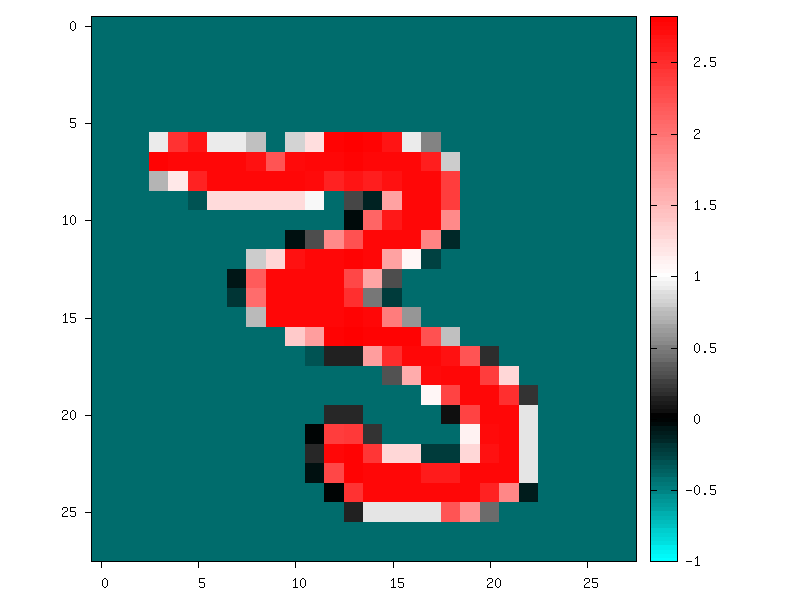
\includegraphics[width=0.8\linewidth]{figs/frame0Mean1StdDev.png}
  \caption{Image of the set after normalization.}
  \label{fig:frame0Mean1StdDev}
\end{figure}


\subsubsection{Substracting the mean image of the set}

Using the \lstinline!StimuliData! object followed with an
\lstinline!AffineTransformation!, it is also possible to use the mean image of
 the dataset to normalize the data:
\begin{lstlisting}[language=ini]
[env.StimuliData-meanData]
ApplyTo=LearnOnly
MeanData=1 ; Provides the _MeanData parameter used in the transformation

[env.Transformation]
Type=AffineTransformation
FirstOperator=Minus
FirstValue=[env.StimuliData-meanData]_MeanData
\end{lstlisting}

The resulting global mean image can be visualized in
 \emph{env.StimuliData-meanData/meanData.bin.png} an is shown in figure
 \ref{fig:meanData}.

\begin{figure}[ht!]
  \centering
  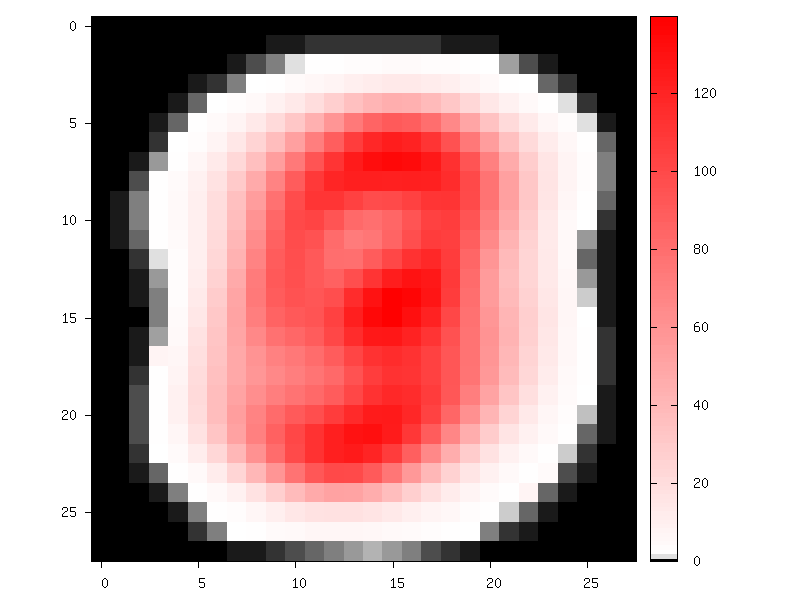
\includegraphics[width=0.8\linewidth]{figs/meanData.png}
  \caption{Global mean image generated by \lstinline!StimuliData! with
  the \lstinline!MeanData! parameter enabled.}
  \label{fig:meanData}
\end{figure}

After this transformation, the reported stimuli data becomes:
\begin{lstlisting}[style=console]
env.StimuliData-processed data:
Number of stimuli: 60000
Data width range: [28, 28]
Data height range: [28, 28]
Data channels range: [1, 1]
Value range: [-139.554, 254.979]
Value mean: -3.45583e-08
Value std. dev.: 66.1288
\end{lstlisting}

The result of the transformation on the first images of the set can be checked
 in the generated \emph{frames} folder, as shown in figure
  \ref{fig:frameMinusMean}.

\begin{figure}[!htb]
  \centering
  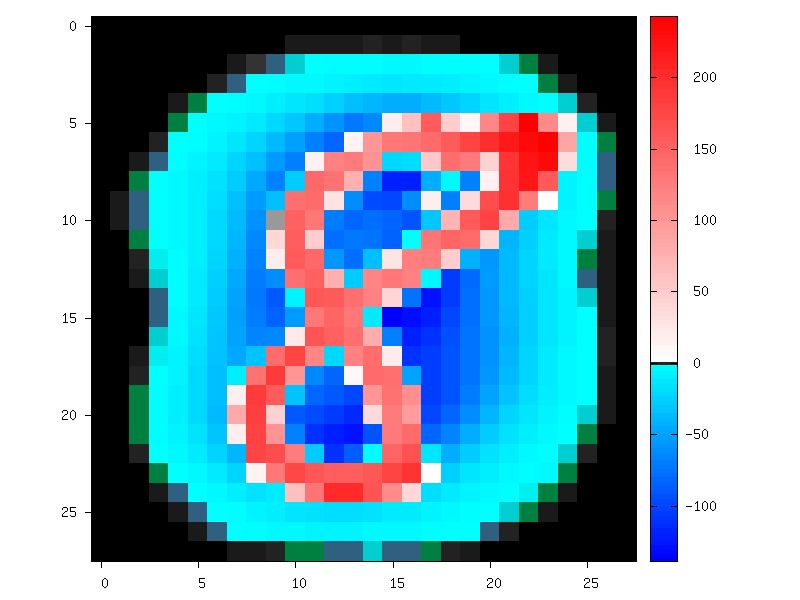
\includegraphics[width=0.8\linewidth]{figs/frameMinusMean.png}
  \caption{Image of the set after the \lstinline!AffineTransformation!
  substracting the global mean image (keep in mind that the original image
  value range is [0, 255]).}
  \label{fig:frameMinusMean}
\end{figure}


\subsection{Environment}

The environment simply specify the input data format of the network (width,
height and batch size). Example:
\begin{lstlisting}[language=ini]
[env]
SizeX=24
SizeY=24
BatchSize=12 ; [default: 1]
\end{lstlisting}


\begin{center}
 \begin{longtable}{| p{5cm} | p{10cm} | }
 \hline
 Option [default value] & Description\\
 \hline\hline
  \cellcolor{requiredcolor}
  \lstinline!SizeX! & Environment width \\
  \cellcolor{requiredcolor}
  \lstinline!SizeY! & Environment height \\
  \lstinline!NbChannels! [1] & Number of channels (applicable only if there is
   no \lstinline!env.ChannelTransformation[...]!) \\
  \lstinline!BatchSize! [1] & Batch size \\
  \lstinline!CompositeStimuli! [0] & If true, use pixel-wise stimuli labels \\
  \lstinline!CachePath! [] & Stimuli cache path (no cache if left empty) \\
  \hline
  \lstinline!StimulusType! [\lstinline!SingleBurst!] & Method for converting
  stimuli into spike trains. Can be any of \lstinline!SingleBurst!,
   \lstinline!Periodic!, \lstinline!JitteredPeriodic! or
   \lstinline!Poissonian! \\
  \lstinline!DiscardedLateStimuli! [1.0] & The pixels in the pre-processed
  stimuli with a value above this limit never generate spiking events \\
  \lstinline!PeriodMeanMin! [50 \lstinline!TimeMs!] & Mean minimum period
  $\overline{T_{min}}$, used for periodic temporal codings, corresponding to
  pixels in the pre-processed stimuli with a value of 0 (which are supposed to
   be the most significant pixels) \\
  \lstinline!PeriodMeanMax! [12 \lstinline!TimeS!] & Mean maximum period
  $\overline{T_{max}}$, used for periodic temporal codings, corresponding to
  pixels in the pre-processed stimuli with a value of 1 (which are supposed
  to be the least significant pixels). This maximum period may be never reached
   if \lstinline!DiscardedLateStimuli! is lower than 1.0 \\
  \lstinline!PeriodRelStdDev! [0.1] & Relative standard deviation, used for
  periodic temporal codings, applied to the spiking period of a pixel \\
  \lstinline!PeriodMin! [11 \lstinline!TimeMs!] & Absolute minimum period,
  or spiking interval, used for periodic temporal codings, for any pixel \\
 \hline
\end{longtable}
\end{center}

\subsubsection{\label{sec:transformations}Built-in transformations}

There are 6 possible categories of transformations:
\begin{myitemize}
\item \lstinline!env.Transformation[...]! Transformations applied to the
input images before channels creation;
\item \lstinline!env.OnTheFlyTransformation[...]! On-the-fly transformations
applied to the input images before channels creation;
\item \lstinline!env.ChannelTransformation[...]! Create or add transformation
for a specific channel;
\item \lstinline!env.ChannelOnTheFlyTransformation[...]! Create or add
on-the-fly transformation for a specific channel;
\item \lstinline!env.ChannelsTransformation[...]! Transformations applied to
all the channels of the input images;
\item \lstinline!env.ChannelsOnTheFlyTransformation[...]! On-the-fly
transformations applied to all the channels of the input images.
\end{myitemize}

Example:
\begin{lstlisting}[language=ini]
[env.Transformation]
Type=PadCropTransformation
Width=24
Height=24
\end{lstlisting}

Several transformations can applied successively. In this case, to be able
to apply multiple transformations of the same category, a different suffix
 (\lstinline![...]!) must be added to each transformation.

\textbf{The transformations will be processed in the order of appearance in the
 INI file regardless of their suffix.}

Common set of parameters for any kind of transformation:
\begin{center}
 \begin{longtable}{| p{5cm} | p{10cm} | }
 \hline
 Option [default value] & Description\\
 \hline\hline
  \lstinline!ApplyTo! [\lstinline!All!] & Apply the transformation only to the
  specified stimuli sets. Can be: \\
    & \lstinline!LearnOnly!: learning set only \\
    & \lstinline!ValidationOnly!: validation set only \\
    & \lstinline!TestOnly!: testing set only \\
    & \lstinline!NoLearn!: validation and testing sets only \\
    & \lstinline!NoValidation!: learning and testing sets only \\
    & \lstinline!NoTest!: learning and validation sets only \\
    & \lstinline!All!: all sets (default) \\
 \hline
\end{longtable}
\end{center}

Example:
\begin{lstlisting}[language=ini]
[env.Transformation-1]
Type=ChannelExtractionTransformation
CSChannel=Gray

[env.Transformation-2]
Type=RescaleTransformation
Width=29
Height=29

[env.Transformation-3]
Type=EqualizeTransformation

[env.OnTheFlyTransformation]
Type=DistortionTransformation
ApplyTo=LearnOnly ; Apply this transformation for the Learning set only
ElasticGaussianSize=21
ElasticSigma=6.0
ElasticScaling=20.0
Scaling=15.0
Rotation=15.0
\end{lstlisting}


List of available transformations:

\paragraph{\texorpdfstring{%%
\lstinline[basicstyle=\ttfamily\bfseries]!AffineTransformation!}
{AffineTransformation}}
Apply an element-wise affine transformation to the image with matrixes of the
 same size.

\begin{center}
 \begin{tabular}{| p{5cm} | p{10cm} | }
 \hline
 Option [default value] & Description\\
 \hline\hline
  \cellcolor{requiredcolor}
  \lstinline!FirstOperator! & First element-wise operator, can be
  \lstinline!Plus!, \lstinline!Minus!, \lstinline!Multiplies!,
  \lstinline!Divides!  \\
  \cellcolor{requiredcolor}
  \lstinline!FirstValue! & First matrix file name \\
  \lstinline!SecondOperator! [\lstinline!Plus!] & Second element-wise operator,
  can be \lstinline!Plus!, \lstinline!Minus!, \lstinline!Multiplies!,
  \lstinline!Divides!  \\
  \lstinline!SecondValue! [] & Second matrix file name \\
 \hline
\end{tabular}
\end{center}

The final operation is the following, with $A$ the image matrix, $B_{1st}$,
$B_{2nd}$ the matrixes to add/substract/multiply/divide and $\odot$ the
element-wise operator :
\[f(A) = \left(A\;\substack{\odot\\op_{1st}}\;B_{1st}\right)\;
\substack{\odot\\op_{2nd}}\;B_{2nd}\]


\paragraph{\texorpdfstring{%%
\lstinline[basicstyle=\ttfamily\bfseries]!ApodizationTransformation!}
{ApodizationTransformation}}
Apply an apodization window to each data row.

\begin{center}
 \begin{tabular}{| p{5cm} | p{10cm} | }
 \hline
 Option [default value] & Description\\
 \hline\hline
  \cellcolor{requiredcolor}
  \lstinline!Size! & Window total size (must match the number of data
  columns) \\
  \lstinline!WindowName! [\lstinline!Rectangular!] & Window name.
  Possible values are: \\
   & \lstinline!Rectangular!: Rectangular \\
   & \lstinline!Hann!: Hann \\
   & \lstinline!Hamming!: Hamming \\
   & \lstinline!Cosine!: Cosine \\
   & \lstinline!Gaussian!: Gaussian \\
   & \lstinline!Blackman!: Blackman \\
   & \lstinline!Kaiser!: Kaiser \\
 \hline
\end{tabular}
\end{center}


\subparagraph{\texorpdfstring{%%
\lstinline[basicstyle=\ttfamily\bfseries]!Gaussian! window}{Gaussian window}}
Gaussian window.

\begin{center}
 \begin{tabular}{| m{4cm} | m{7cm} | }
 \hline
 Option [default value] & Description\\
 \hline\hline
  \emph{WindowName}\lstinline!.Sigma! [0.4] & Sigma\\
 \hline
\end{tabular}
\end{center}


\subparagraph{\texorpdfstring{%%
\lstinline[basicstyle=\ttfamily\bfseries]!Blackman! window}{Blackman window}}
Blackman window.

\begin{center}
 \begin{tabular}{| m{4cm} | m{7cm} | }
 \hline
 Option [default value] & Description\\
 \hline\hline
  \emph{WindowName}\lstinline!.Alpha! [0.16] & Alpha\\
 \hline
\end{tabular}
\end{center}


\subparagraph{\texorpdfstring{%%
\lstinline[basicstyle=\ttfamily\bfseries]!Kaiser! window}{Kaiser window}}
Kaiser window.

\begin{center}
 \begin{tabular}{| m{4cm} | m{7cm} | }
 \hline
 Option [default value] & Description\\
 \hline\hline
  \emph{WindowName}\lstinline!.Beta! [5.0] & Beta\\
 \hline
\end{tabular}
\end{center}


\paragraph{\texorpdfstring{%%
\lstinline[basicstyle=\ttfamily\bfseries]!ChannelExtractionTransformation!}
{ChannelExtractionTransformation}}
Extract an image channel.

\begin{center}
 \begin{tabular}{| p{5cm} | p{10cm} | }
 \hline
 Option & Description\\
 \hline\hline
  \cellcolor{requiredcolor}\lstinline!CSChannel! & \lstinline!Blue!: blue
  channel in the BGR colorspace, or first channel of any colorspace \\
 & \lstinline!Green!: green channel in the BGR colorspace, or second channel
 of any colorspace \\
 & \lstinline!Red!: red channel in the BGR colorspace, or third channel of any
  colorspace \\
 & \lstinline!Hue!: hue channel in the HSV colorspace \\
 & \lstinline!Saturation!: saturation channel in the HSV colorspace \\
 & \lstinline!Value!: value channel in the HSV colorspace \\
 & \lstinline!Gray!: gray conversion \\
 & \lstinline!Y!: Y channel in the YCbCr colorspace \\
 & \lstinline!Cb!: Cb channel in the YCbCr colorspace \\
 & \lstinline!Cr!: Cr channel in the YCbCr colorspace \\
 \hline
\end{tabular}
\end{center}

\paragraph{\texorpdfstring{%%
\lstinline[basicstyle=\ttfamily\bfseries]!ColorSpaceTransformation!}
{ColorSpaceTransformation}}
Change the current image colorspace.

\begin{center}
 \begin{tabular}{| p{5cm} | p{10cm} | }
 \hline
 Option & Description\\
 \hline\hline
  \cellcolor{requiredcolor}\lstinline!ColorSpace! & \lstinline!BGR!: if the
  image is in grayscale, convert it in BGR \\
 & \lstinline!HSV! \\
 & \lstinline!HLS! \\
 & \lstinline!YCrCb! \\
 & \lstinline!CIELab! \\
 & \lstinline!CIELuv! \\
 \hline
\end{tabular}
\end{center}


\paragraph{\texorpdfstring{%%
\lstinline[basicstyle=\ttfamily\bfseries]!DFTTransformation!}
{DFTTransformation}}
Apply a DFT to the data.
The input data must be single channel, the resulting data is two channels,
the first for the real part and the second for the imaginary part.

\begin{center}
 \begin{tabular}{| p{5cm} | p{10cm} | }
 \hline
 Option [default value] & Description\\
 \hline\hline
  \lstinline!TwoDimensional! [1] & If true, compute a 2D image DFT. Otherwise,
   compute the 1D DFT of each data row \\
 \hline
\end{tabular}
\end{center}

Note that this transformation can add zero-padding if required by the underlying
 FFT implementation.


\paragraph{\label{par:DistortionTransformation}%
\texorpdfstring{\lstinline[basicstyle=\ttfamily\bfseries]!DistortionTransformation!\protect\iponly}
{DistortionTransformation}}
Apply elastic distortion to the image. This transformation is generally used
on-the-fly (so that a different distortion is performed for each image), and
for the learning only.


\begin{center}
 \begin{tabular}{| p{5cm} | p{10cm} | }
 \hline
 Option [default value] & Description\\
 \hline\hline
  \lstinline!ElasticGaussianSize! [15] & Size of the gaussian for elastic
  distortion (in pixels) \\
  \lstinline!ElasticSigma! [6.0] & Sigma of the gaussian for elastic
  distortion \\
  \lstinline!ElasticScaling! [0.0] & Scaling of the gaussian for elastic
  distortion \\
  \lstinline!Scaling! [0.0] & Maximum random scaling amplitude
  (+/-, in percentage) \\
  \lstinline!Rotation! [0.0] & Maximum random rotation amplitude
  (+/-, in °) \\
 \hline
\end{tabular}
\end{center}

\paragraph{\texorpdfstring{%%
\lstinline[basicstyle=\ttfamily\bfseries]!EqualizeTransformation!%%
\protect\iponly}{EqualizeTransformation}}
Image histogram equalization.

\begin{center}
 \begin{tabular}{| p{5cm} | p{10cm} | }
 \hline
 Option [default value] & Description\\
 \hline\hline
  \lstinline!Method! [\lstinline!Standard!] & \lstinline!Standard!: standard
  histogram equalization \\
   & \lstinline!CLAHE!: contrast limited adaptive histogram equalization \\
  \lstinline!CLAHE_ClipLimit! [40.0] & Threshold for contrast limiting
  (for \lstinline!CLAHE! only) \\
  \lstinline!CLAHE_GridSize! [8] & Size of grid for histogram equalization
   (for \lstinline!CLAHE! only).
  Input image will be divided into equally sized rectangular tiles.
  This parameter defines the number of tiles in row and column. \\
 \hline
\end{tabular}
\end{center}


\paragraph{\texorpdfstring{%%
\lstinline[basicstyle=\ttfamily\bfseries]!ExpandLabelTransformation!%%
\protect\iponly}{ExpandLabelTransformation}}
Expand single image label (1x1 pixel) to full frame label.


\paragraph{\texorpdfstring{%%
\lstinline[basicstyle=\ttfamily\bfseries]!FilterTransformation!}
{FilterTransformation}}
Apply a convolution filter to the image.

\begin{center}
 \begin{tabular}{| p{5cm} | p{10cm} | }
 \hline
 Option [default value] & Description\\
 \hline\hline
  \cellcolor{requiredcolor}\lstinline!Kernel! & Convolution kernel.
  Possible values are: \\
   & \lstinline!*!: custom kernel \\
   & \lstinline!Gaussian!: Gaussian kernel \\
   & \lstinline!LoG!: Laplacian Of Gaussian kernel \\
   & \lstinline!DoG!: Difference Of Gaussian kernel \\
   & \lstinline!Gabor!: Gabor kernel \\
 \hline
\end{tabular}
\end{center}


\subparagraph{\texorpdfstring{%%
\lstinline[basicstyle=\ttfamily\bfseries]!*! kernel}{* kernel}}
Custom kernel.

\begin{center}
 \begin{tabular}{| m{4cm} | m{7cm} | }
 \hline
 Option & Description\\
 \hline\hline
  \lstinline!Kernel.SizeX! [0] & Width of the kernel (numer of columns)\\
  \lstinline!Kernel.SizeY! [0] & Height of the kernel (number of rows)\\
  \cellcolor{requiredcolor}\lstinline!Kernel.Mat! & List of row-major ordered
   coefficients of the kernel\\
 \hline
\end{tabular}
\end{center}

If both \lstinline!Kernel.SizeX! and \lstinline!Kernel.SizeY! are 0, the kernel
 is assumed to be square.


\subparagraph{\texorpdfstring{%%
\lstinline[basicstyle=\ttfamily\bfseries]!Gaussian! kernel}{Gaussian kernel}}
Gaussian kernel.

\begin{center}
 \begin{tabular}{| m{4cm} | m{7cm} | }
 \hline
 Option [default value] & Description\\
 \hline\hline
  \cellcolor{requiredcolor}\lstinline!Kernel.SizeX! & Width of the kernel
  (numer of columns)\\
  \cellcolor{requiredcolor}\lstinline!Kernel.SizeY! & Height of the kernel
  (number of rows)\\
  \lstinline!Kernel.Positive! [1] & If true, the center of the kernel is
  positive\\
  \lstinline!Kernel.Sigma! [$\sqrt{2.0}$] & Sigma of the kernel\\
 \hline
\end{tabular}
\end{center}


\subparagraph{\texorpdfstring{%%
\lstinline[basicstyle=\ttfamily\bfseries]!LoG! kernel}{LoG kernel}}
Laplacian Of Gaussian kernel.

\begin{center}
 \begin{tabular}{| m{4cm} | m{7cm} | }
 \hline
 Option [default value] & Description\\
 \hline\hline
  \cellcolor{requiredcolor}\lstinline!Kernel.SizeX! & Width of the kernel
  (numer of columns)\\
  \cellcolor{requiredcolor}\lstinline!Kernel.SizeY! & Height of the kernel
  (number of rows)\\
  \lstinline!Kernel.Positive! [1] & If true, the center of the kernel is
  positive\\
  \lstinline!Kernel.Sigma! [$\sqrt{2.0}$] & Sigma of the kernel\\
 \hline
\end{tabular}
\end{center}

\subparagraph{\texorpdfstring{%%
\lstinline[basicstyle=\ttfamily\bfseries]!DoG! kernel}{DoG kernel}}
Difference Of Gaussian kernel kernel.

\begin{center}
 \begin{tabular}{| m{4cm} | m{7cm} | }
 \hline
 Option [default value] & Description\\
 \hline\hline
  \cellcolor{requiredcolor}\lstinline!Kernel.SizeX! & Width of the kernel
  (numer of columns)\\
  \cellcolor{requiredcolor}\lstinline!Kernel.SizeY! & Height of the kernel
   (number of rows)\\
  \lstinline!Kernel.Positive! [1] & If true, the center of the kernel is
  positive\\
  \lstinline!Kernel.Sigma1! [2.0] & Sigma1 of the kernel\\
  \lstinline!Kernel.Sigma2! [1.0] & Sigma2 of the kernel\\
 \hline
\end{tabular}
\end{center}


\subparagraph{\texorpdfstring{%%
\lstinline[basicstyle=\ttfamily\bfseries]!Gabor! kernel}{Gabor kernel}}
Gabor kernel.

\begin{center}
 \begin{tabular}{| m{4cm} | m{7cm} | }
 \hline
 Option [default value] & Description\\
 \hline\hline
  \cellcolor{requiredcolor}\lstinline!Kernel.SizeX! & Width of the kernel
  (numer of columns)\\
  \cellcolor{requiredcolor}\lstinline!Kernel.SizeY! & Height of the kernel
  (number of rows)\\
  \cellcolor{requiredcolor}\lstinline!Kernel.Theta! & Theta of the kernel\\
  \lstinline!Kernel.Sigma! [$\sqrt{2.0}$] & Sigma of the kernel\\
  \lstinline!Kernel.Lambda! [10.0] & Lambda of the kernel\\
  \lstinline!Kernel.Psi! [$\pi/2.0$] & Psi of the kernel\\
  \lstinline!Kernel.Gamma! [0.5] & Gamma of the kernel\\
 \hline
\end{tabular}
\end{center}


\paragraph{\texorpdfstring{%%
\lstinline[basicstyle=\ttfamily\bfseries]!FlipTransformation!}
{FlipTransformation}}
Image flip transformation.

\begin{center}
 \begin{tabular}{| p{5cm} | p{10cm} | }
 \hline
 Option [default value] & Description\\
 \hline\hline
  \lstinline!HorizontalFlip! [0] & If true, flip the image horizontally \\
  \lstinline!VerticalFlip! [0] & If true, flip the image vertically \\
  \lstinline!RandomHorizontalFlip! [0] & If true, randomly flip the image
   horizontally \\
  \lstinline!RandomVerticalFlip! [0] & If true, randomly flip the image
  vertically \\
 \hline
\end{tabular}
\end{center}


\paragraph{\texorpdfstring{%%
\lstinline[basicstyle=\ttfamily\bfseries]!GradientFilterTransformation!%%
\protect\iponly}{GradientFilterTransformation}}
Compute image gradient.

\begin{center}
 \begin{tabular}{| p{5cm} | p{10cm} | }
 \hline
 Option [default value] & Description\\
 \hline\hline
  \lstinline!Scale! [1.0] & Scale to apply to the computed gradient \\
  \lstinline!Delta! [0.0] & Bias to add to the computed gradient \\
  \lstinline!GradientFilter! [\lstinline!Sobel!] & Filter type to use for
  computing the gradient. Possible options are: \lstinline!Sobel!,
  \lstinline!Scharr! and \lstinline!Laplacian! \\
  \lstinline!KernelSize! [3] & Size of the filter kernel (has no effect when
  using the \lstinline!Scharr! filter, which kernel size is always 3x3) \\
  \lstinline!ApplyToLabels! [0] & If true, use the computed gradient to filter
  the image label and ignore pixel areas where the gradient is below the
   \lstinline!Threshold!. In this case, only the labels are modified, not the
    image \\\hline
  \lstinline!InvThreshold! [0] & If true, ignored label pixels will be the ones
  with a low gradient (low contrasted areas) \\
  \lstinline!Threshold! [0.5] & Threshold applied on the image gradient \\
  \lstinline!Label! [] & List of labels to filter (space-separated) \\
  \lstinline!GradientScale! [1.0] & Rescale the image by this factor before
  applying the gradient and the threshold, then scale it back to filter the
   labels \\
 \hline
\end{tabular}
\end{center}


\paragraph{\texorpdfstring{%%
\lstinline[basicstyle=\ttfamily\bfseries]!LabelSliceExtractionTransformation!%%
\protect\iponly}{LabelSliceExtractionTransformation}}
Extract a slice from an image belonging to a given label.

\begin{center}
 \begin{tabular}{| p{5cm} | p{10cm} | }
 \hline
 Option [default value] & Description\\
 \hline\hline
  \cellcolor{requiredcolor}\lstinline!Width! & Width of the slice to extract \\
  \cellcolor{requiredcolor}\lstinline!Height! & Height of the slice to
  extract \\
  \lstinline!Label! [-1] & Slice should belong to this label ID. If -1, the
  label ID is random \\
 \hline
\end{tabular}
\end{center}



\paragraph{\texorpdfstring{%%
\lstinline[basicstyle=\ttfamily\bfseries]!MagnitudePhaseTransformation!}
{MagnitudePhaseTransformation}}
Compute the magnitude and phase of a complex two channels input data, with the
first channel $x$ being the real part and the second channel $y$ the imaginary
part. The resulting data is two channels, the first one with the magnitude and
 the second one with the phase.

\begin{center}
 \begin{tabular}{| p{5cm} | p{10cm} | }
 \hline
 Option [default value] & Description\\
 \hline\hline
  \lstinline!LogScale! [0] & If true, compute the magnitude in log scale \\
 \hline
\end{tabular}
\end{center}

The magnitude is:

\[ M_{i,j} = \sqrt{x_{i,j}^2 + x_{i,j}^2} \]

If \lstinline!LogScale! = 1, compute $M'_{i,j} = log(1 + M_{i,j})$.

The phase is:

\[ \theta_{i,j} = atan2(y_{i,j}, x_{i,j}) \]



\paragraph{\texorpdfstring{%%
\lstinline[basicstyle=\ttfamily\bfseries]
!MorphologicalReconstructionTransformation!\protect\iponly}
{MorphologicalReconstructionTransformation}}
Apply a morphological reconstruction transformation to the image.
This transformation is also useful for post-processing.

\begin{center}
 \begin{tabular}{| p{5cm} | p{10cm} | }
 \hline
 Option [default value] & Description\\
 \hline\hline
  \cellcolor{requiredcolor}\lstinline!Operation! & Morphological operation to
  apply. Can be:\\
   & \lstinline!ReconstructionByErosion!: reconstruction by erosion operation \\
   & \lstinline!ReconstructionByDilation!: reconstruction by dilation
   operation \\
   & \lstinline!OpeningByReconstruction!: opening by reconstruction operation \\
   & \lstinline!ClosingByReconstruction!: closing by reconstruction operation \\
  \cellcolor{requiredcolor}\lstinline!Size! & Size of the structuring element \\
  \lstinline!ApplyToLabels! [0] & If true, apply the transformation to the
  labels instead of the image \\
  \lstinline!Shape! [\lstinline!Rectangular!] & Shape of the structuring element
   used for morphology operations. Can be \lstinline!Rectangular!,
   \lstinline!Elliptic! or \lstinline!Cross!. \\
  \lstinline!NbIterations! [1] & Number of times erosion and dilation are
  applied for opening and closing reconstructions \\
 \hline
\end{tabular}
\end{center}


\paragraph{\texorpdfstring{\lstinline[basicstyle=\ttfamily\bfseries]!MorphologyTransformation!\protect\iponly}
{MorphologyTransformation}}
Apply a morphology transformation to the image.
This transformation is also useful for post-processing.

\begin{center}
 \begin{tabular}{| p{5cm} | p{10cm} | }
 \hline
 Option [default value] & Description\\
 \hline\hline
  \cellcolor{requiredcolor}\lstinline!Operation! & Morphological operation to
  apply. Can be:\\
   & \lstinline!Erode!: erode operation ($=erode(src)$) \\
   & \lstinline!Dilate!: dilate operation ($=dilate(src)$) \\
   & \lstinline!Opening!: opening operation ($open(src)=dilate(erode(src))$) \\
   & \lstinline!Closing!: closing operation ($close(src)=erode(dilate(src))$) \\
   & \lstinline!Gradient!: morphological gradient ($=dilate(src)-erode(src)$) \\
   & \lstinline!TopHat!: top hat ($=src-open(src)$) \\
   & \lstinline!BlackHat!: black hat ($=close(src)-src$) \\
  \cellcolor{requiredcolor}\lstinline!Size! & Size of the structuring element \\
  \lstinline!ApplyToLabels! [0] & If true, apply the transformation to the
  labels instead of the image \\
  \lstinline!Shape! [\lstinline!Rectangular!] & Shape of the structuring element
   used for morphology operations. Can be \lstinline!Rectangular!,
   \lstinline!Elliptic! or \lstinline!Cross!. \\
  \lstinline!NbIterations! [1] & Number of times erosion and dilation are
  applied \\
 \hline
\end{tabular}
\end{center}


\paragraph{\texorpdfstring{\lstinline[basicstyle=\ttfamily\bfseries]!NormalizeTransformation!}{NormalizeTransformation}}
Normalize the image.

\begin{center}
 \begin{tabular}{| p{5cm} | p{10cm} | }
 \hline
 Option [default value] & Description\\
 \hline\hline
  \lstinline!Norm! [\lstinline!MinMax!] & Norm type, can be: \\
   & \lstinline!L1!: L1 normalization \\
   & \lstinline!L2!: L2 normalization \\
   & \lstinline!Linf!: Linf normalization \\
   & \lstinline!MinMax!: min-max normalization \\
  \lstinline!NormValue! [1.0] & Norm value (for \lstinline!L1!, \lstinline!L2!
   and \lstinline!Linf!) \\
   & Such that $||data||_{L_{p}} = NormValue$ \\
  \lstinline!NormMin! [0.0] & Min value (for \lstinline!MinMax! only) \\
   & Such that $min(data) = NormMin$ \\
  \lstinline!NormMax! [1.0] & Max value (for \lstinline!MinMax! only) \\
   & Such that $max(data) = NormMax$ \\
  \lstinline!PerChannel! [0] & If true, normalize each channel individually \\
 \hline
\end{tabular}
\end{center}


\paragraph{\texorpdfstring{%%
\lstinline[basicstyle=\ttfamily\bfseries]!PadCropTransformation!}
{PadCropTransformation}}
Pad/crop the image to a specified size.

\begin{center}
 \begin{tabular}{| p{5cm} | p{10cm} | }
 \hline
 Option [default value] & Description\\
 \hline\hline
  \cellcolor{requiredcolor}\lstinline!Width! & Width of the padded/cropped
  image \\
  \cellcolor{requiredcolor}\lstinline!Height! & Height of the padded/cropped
   image \\
  \lstinline!PaddingBackground! [\lstinline!MeanColor!] & Background color
  used when padding. Possible values: \\
   & \lstinline!MeanColor!: pad with the mean color of the image \\
   & \lstinline!BlackColor!: pad with black \\
 \hline
\end{tabular}
\end{center}

\paragraph{\texorpdfstring{%%
\lstinline[basicstyle=\ttfamily\bfseries]!RandomAffineTransformation!%%
\protect\iponly}{RandomAffineTransformation}}
Apply a global random affine transformation to the values of the image.

\begin{center}
 \begin{tabular}{| p{5cm} | p{10cm} | }
 \hline
 Option [default value] & Description\\
 \hline\hline
  \cellcolor{requiredcolor}\lstinline!GainVar! & Random gain is in range $\pm$\lstinline!GainVar! \\
  \lstinline!BiasVar! [0.0] & Random bias is in range $\pm$\lstinline!BiasVar!\\
 \hline
\end{tabular}
\end{center}


\paragraph{\texorpdfstring{%%
\lstinline[basicstyle=\ttfamily\bfseries]!RangeAffineTransformation!}
{RangeAffineTransformation}}
Apply an affine transformation to the values of the image.

\begin{center}
 \begin{tabular}{| p{5cm} | p{10cm} | }
 \hline
 Option [default value] & Description\\
 \hline\hline
  \cellcolor{requiredcolor}\lstinline!FirstOperator! & First operator, can be
   \lstinline!Plus!, \lstinline!Minus!, \lstinline!Multiplies!,
   \lstinline!Divides!  \\
  \cellcolor{requiredcolor}\lstinline!FirstValue! & First value \\
  \lstinline!SecondOperator! [\lstinline!Plus!] & Second operator, can be
  \lstinline!Plus!, \lstinline!Minus!, \lstinline!Multiplies!,
  \lstinline!Divides!  \\
  \lstinline!SecondValue! [0.0] & Second value \\
 \hline
\end{tabular}
\end{center}

The final operation is the following:
\[f(x) = \left(x\;\substack{o\\op_{1st}}\;val_{1st}\right)\;
\substack{o\\op_{2nd}}\;val_{2nd}\]

\paragraph{\texorpdfstring{\lstinline[basicstyle=\ttfamily\bfseries]!RangeClippingTransformation!\protect\iponly}
{RangeClippingTransformation}}
Clip the value range of the image.

\begin{center}
 \begin{tabular}{| p{5cm} | p{10cm} | }
 \hline
 Option [default value] & Description\\
 \hline\hline
  \lstinline!RangeMin! [$min(data)$] & Image values below \lstinline!RangeMin!
  are clipped to 0 \\
  \lstinline!RangeMax! [$max(data)$] & Image values above \lstinline!RangeMax!
   are clipped to 1 (or the maximum integer value of the data type) \\
 \hline
\end{tabular}
\end{center}

\paragraph{\texorpdfstring{%%
\lstinline[basicstyle=\ttfamily\bfseries]!RescaleTransformation!}
{RescaleTransformation}}
Rescale the image to a specified size.

\begin{center}
 \begin{tabular}{| p{5cm} | p{10cm} | }
 \hline
 Option [default value] & Description\\
 \hline\hline
  \cellcolor{requiredcolor}\lstinline!Width! & Width of the rescaled image \\
  \cellcolor{requiredcolor}\lstinline!Height! & Height of the rescaled image \\
  \lstinline!KeepAspectRatio! [0] & If true, keeps the aspect ratio of the
  image \\
  \lstinline!ResizeToFit! [1] & If true, resize along the longest dimension
  when \lstinline!KeepAspectRatio! is true \\
 \hline
\end{tabular}
\end{center}

\paragraph{\texorpdfstring{%%
\lstinline[basicstyle=\ttfamily\bfseries]!ReshapeTransformation!}
{ReshapeTransformation}}
Reshape the data to a specified size.

\begin{center}
 \begin{tabular}{| p{5cm} | p{10cm} | }
 \hline
 Option [default value] & Description\\
 \hline\hline
  \cellcolor{requiredcolor}\lstinline!NbRows! & New number of rows \\
  \lstinline!NbCols! [0] & New number of cols (0 = no check) \\
  \lstinline!NbChannels! [0] & New number of channels (0 = no change) \\
 \hline
\end{tabular}
\end{center}

\paragraph{\texorpdfstring{%%
\lstinline[basicstyle=\ttfamily\bfseries]!SliceExtractionTransformation!%%
\protect\iponly}{SliceExtractionTransformation}}
Extract a slice from an image.

\begin{center}
 \begin{tabular}{| p{5cm} | p{10cm} | }
 \hline
 Option [default value] & Description\\
 \hline\hline
  \cellcolor{requiredcolor}\lstinline!Width! & Width of the slice to extract \\
  \cellcolor{requiredcolor}\lstinline!Height! & Height of the slice to
  extract \\
  \lstinline!OffsetX! [0] & X offset of the slice to extract \\
  \lstinline!OffsetY! [0] & Y offset of the slice to extract \\
  \lstinline!RandomOffsetX! [0] & If true, the X offset is chosen randomly \\
  \lstinline!RandomOffsetY! [0] & If true, the Y offset is chosen randomly \\
  \lstinline!AllowPadding! [0] & If true, zero-padding is allowed if the image
  is smaller than the slice to extract \\
 \hline
\end{tabular}
\end{center}



\paragraph{\texorpdfstring{\lstinline[basicstyle=\ttfamily\bfseries]!ThresholdTransformation!}{ThresholdTransformation}}
Apply a thresholding transformation to the image.
This transformation is also useful for post-processing.

\begin{center}
 \begin{tabular}{| p{5cm} | p{10cm} | }
 \hline
 Option [default value] & Description\\
 \hline\hline
  \cellcolor{requiredcolor}\lstinline!Threshold! & Threshold value \\
  \lstinline!OtsuMethod! [0] & Use Otsu's method to determine the optimal
  threshold (if true, the \lstinline!Threshold! value is ignored) \\
  \lstinline!Operation! [Binary] & Thresholding operation to apply. Can be:\\
   & \lstinline!Binary! \\
   & \lstinline!BinaryInverted! \\
   & \lstinline!Truncate! \\
   & \lstinline!ToZero! \\
   & \lstinline!ToZeroInverted! \\
  \lstinline!MaxValue! [1.0] & Max. value to use with \lstinline!Binary! and \lstinline!BinaryInverted! operations \\
 \hline
\end{tabular}
\end{center}


\paragraph{\texorpdfstring{%%
\lstinline[basicstyle=\ttfamily\bfseries]!TrimTransformation!}
{TrimTransformation}}
Trim the image.

\begin{center}
 \begin{tabular}{| p{5cm} | p{10cm} | }
 \hline
 Option [default value] & Description\\
 \hline\hline
  \cellcolor{requiredcolor}\lstinline!NbLevels! & Number of levels for the color discretization of the image \\
  \lstinline!Method! [\lstinline!Discretize!] & Possible values are: \\
   & \lstinline!Reduce!: discretization using K-means \\
   & \lstinline!Discretize!: simple discretization \\
 \hline
\end{tabular}
\end{center}


\paragraph{\texorpdfstring{%%
\lstinline[basicstyle=\ttfamily\bfseries]!WallisFilterTransformation!%%
\protect\iponly}{WallisFilterTransformation}}
Apply Wallis filter to the image.

\begin{center}
 \begin{tabular}{| p{5cm} | p{10cm} | }
 \hline
 Option [default value] & Description\\
 \hline\hline
  \cellcolor{requiredcolor}\lstinline!Size! & Size of the filter \\
  \lstinline!Mean! [0.0] & Target mean value \\
  \lstinline!StdDev! [1.0] & Target standard deviation \\
  \lstinline!PerChannel! [0] & If true, apply Wallis filter to each channel
  individually (this parameter is meaningful only if \lstinline!Size! is 0) \\
 \hline
\end{tabular}
\end{center}

\subsection{Network layers}

\subsubsection{Layer definition}
Common set of parameters for any kind of layer.

\begin{center}
 \begin{tabular}{| p{5cm} | p{10cm} | }
 \hline
 Option [default value] & Description\\
 \hline\hline
  \cellcolor{requiredcolor}\lstinline!Input! & Name of the section(s) for the
  input layer(s). Comma separated \\
  \cellcolor{requiredcolor}\lstinline!Type! & Type of the layer. Can be any of
  the type described below \\
  \lstinline!Model! [\lstinline!DefaultModel!] & Layer model to use \\
  \lstinline!ConfigSection! [] & Name of the configuration section for layer \\
 \hline
\end{tabular}
\end{center}

To specify that the back-propagated error must be computed at the output of a
given layer (generally the last layer, or output layer), one must add a target
section named \emph{LayerName}\lstinline!.Target!:
\begin{lstlisting}[language=ini]
...
[LayerName.Target]
TargetValue=1.0 ; default: 1.0
DefaultValue=0.0 ; default: -1.0
\end{lstlisting}


\subsubsection{Weight fillers}
Fillers to initialize weights and biases in the different type of layer.

Usage example:
\begin{lstlisting}[language=ini]
[conv1]
...
WeightsFiller=NormalFiller
WeightsFiller.Mean=0.0
WeightsFiller.StdDev=0.05
...
\end{lstlisting}

The initial weights distribution for each layer can be checked in the
 \emph{weights\_init} folder, with an example shown in figure
 \ref{fig:weightsInitDistrib}.

\begin{figure}[!htb]
  \centering
  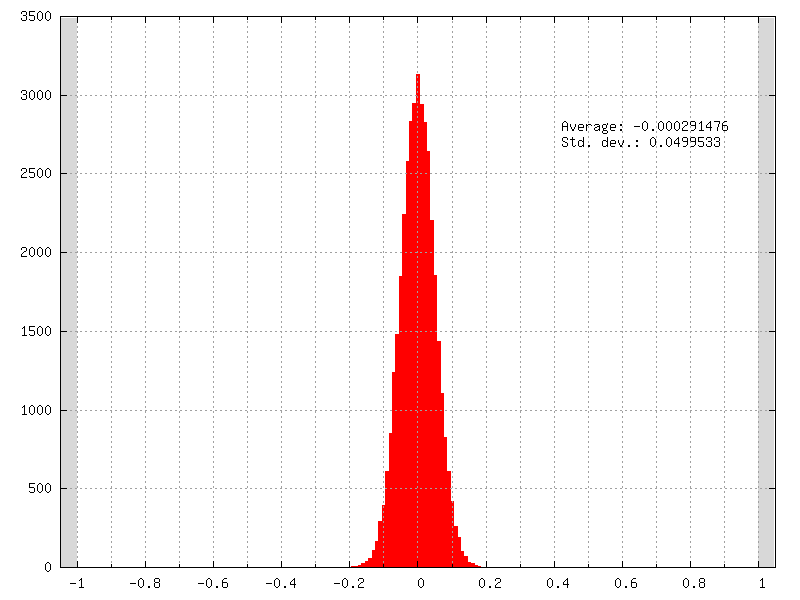
\includegraphics[width=0.8\linewidth]{figs/weightsInitDistrib.png}
  \caption{Initial weights distribution of a layer using a normal distribution
  (\lstinline!NormalFiller!) with a 0 mean and a 0.05 standard deviation.}
  \label{fig:weightsInitDistrib}
\end{figure}


\paragraph{\texorpdfstring{%%
\lstinline[basicstyle=\ttfamily\bfseries]!ConstantFiller!}{ConstantFiller}}
Fill with a constant value.

\begin{center}
 \begin{tabular}{| p{5cm} | p{10cm} | }
 \hline
 Option & Description\\
 \hline\hline
  \cellcolor{requiredcolor}\emph{FillerName}\lstinline!.Value! & Value for the
  filling \\
 \hline
\end{tabular}
\end{center}

\paragraph{\texorpdfstring{%%
\lstinline[basicstyle=\ttfamily\bfseries]!NormalFiller!}{NormalFiller}}
Fill with a normal distribution.

\begin{center}
 \begin{tabular}{| p{5cm} | p{10cm} | }
 \hline
 Option [default value] & Description\\
 \hline\hline
    \emph{FillerName}\lstinline!.Mean! [0.0] & Mean value of the distribution \\
    \emph{FillerName}\lstinline!.StdDev! [1.0] & Standard deviation of the
    distribution \\
 \hline
\end{tabular}
\end{center}

\paragraph{\texorpdfstring{%%
\lstinline[basicstyle=\ttfamily\bfseries]!UniformFiller!}{UniformFiller}}
Fill with an uniform distribution.

\begin{center}
 \begin{tabular}{| p{5cm} | p{10cm} | }
 \hline
 Option [default value] & Description\\
 \hline\hline
    \emph{FillerName}\lstinline!.Min! [0.0] & Min. value \\
    \emph{FillerName}\lstinline!.Max! [1.0] & Max. value \\
 \hline
\end{tabular}
\end{center}


\paragraph{\label{par:XavierFiller}\texorpdfstring{%%
\lstinline[basicstyle=\ttfamily\bfseries]!XavierFiller!}{XavierFiller}}
Fill with an uniform distribution with normalized variance \citep{Glorot2010}.

\begin{center}
 \begin{tabular}{| p{5cm} | p{10cm} | }
 \hline
 Option [default value] & Description\\
 \hline\hline
    \emph{FillerName}\lstinline!.VarianceNorm! [\lstinline!FanIn!]
    & Normalization, can be \lstinline!FanIn!, \lstinline!Average!
    or \lstinline!FanOut! \\
    \emph{FillerName}\lstinline!.Distribution! [\lstinline!Uniform!]
    & Distribution, can be \lstinline!Uniform! or \lstinline!Normal! \\
 \hline
\end{tabular}
\end{center}

Use an uniform distribution with interval $[-scale,scale]$, with $scale = \sqrt{\frac{3.0}{n}}$.

\begin{myitemize}
\item $n$ = $fan\mhyphen{}in$ with \lstinline!FanIn!, resulting in
$Var(W)=\frac{1}{fan\mhyphen{}in}$ \\
\item $n$ = $\frac{(fan\mhyphen{}in + fan\mhyphen{}out)}{2}$ with
\lstinline!Average!, resulting in
$Var(W)=\frac{2}{fan\mhyphen{}in + fan\mhyphen{}out}$ \\
\item $n$ = $fan\mhyphen{}out$ with \lstinline!FanOut!, resulting in
$Var(W)=\frac{1}{fan\mhyphen{}out}$
\end{myitemize}


\subsubsection{\label{sec:WeightSolvers}Weight solvers}

\paragraph{\texorpdfstring{%%
\lstinline[basicstyle=\ttfamily\bfseries]!SGDSolver\_Frame!}{SGDSolver\_Frame}}
SGD Solver for \lstinline!Frame! models.

\begin{center}
 \begin{tabular}{| p{5cm} | p{10cm} | }
 \hline
 Option [default value] & Description\\
 \hline\hline
   \emph{SolverName}\lstinline!.LearningRate! [0.01] & Learning rate \\
   \emph{SolverName}\lstinline!.Momentum! [0.0] & Momentum \\
   \emph{SolverName}\lstinline!.Decay! [0.0] & Decay \\
   \emph{SolverName}\lstinline!.LearningRatePolicy! [\lstinline!None!]
   & Learning rate decay policy. Can be any of \lstinline!None!,
   \lstinline!StepDecay!, \lstinline!ExponentialDecay!, \lstinline!InvTDecay!,
    \lstinline!PolyDecay! \\
   \emph{SolverName}\lstinline!.LearningRateStepSize! [1] & Learning rate
    step size (in number of stimuli) \\
   \emph{SolverName}\lstinline!.LearningRateDecay! [0.1] & Learning rate
    decay \\
   \emph{SolverName}\lstinline!.Clamping! [0] & If true, clamp the weights and
   bias between -1 and 1 \\
   \emph{SolverName}\lstinline!.Power! [0.0] & Polynomial learning rule power
    parameter \\
   \emph{SolverName}\lstinline!.MaxIterations! [0.0] & Polynomial learning
   rule maximum number of iterations \\

 \hline
\end{tabular}
\end{center}

The learning rate decay policies are the following:

\begin{myitemize}
\item \lstinline!StepDecay!: every
\emph{SolverName}\lstinline!.LearningRateStepSize! stimuli, the learning rate
is reduced by a factor \emph{SolverName}\lstinline!.LearningRateDecay!; \\
\item \lstinline!ExponentialDecay!: the learning rate is
$\alpha = \alpha_{0}\exp(-k t)$, with $\alpha_{0}$ the initial learning rate
\emph{SolverName}\lstinline!.LearningRate!, $k$ the rate decay \emph{SolverName}
\lstinline!.LearningRateDecay! and $t$ the step number (one step every
 \emph{SolverName}\lstinline!.LearningRateStepSize! stimuli); \\
\item \lstinline!InvTDecay!: the learning rate is
$\alpha = \alpha_{0} / (1 + k t)$, with $\alpha_{0}$ the initial learning rate
 \emph{SolverName}\lstinline!.LearningRate!, $k$ the rate decay
 \emph{SolverName}\lstinline!.LearningRateDecay! and $t$ the step number
 (one step every \emph{SolverName}\lstinline!.LearningRateStepSize! stimuli). \\
 \item \lstinline!InvDecay!: the learning rate is
$\alpha = \alpha_{0} * (1 + k t)^{-n}$, with $\alpha_{0}$ the initial
learning rate \emph{SolverName}\lstinline!.LearningRate!, $k$ the rate decay
\emph{SolverName}\lstinline!.LearningRateDecay!,
$t$ the current iteration and $n$ the power parameter
\emph{SolverName}\lstinline!.Power! \\
\item \lstinline!PolyDecay!: the learning rate is
$\alpha = \alpha_{0} * (1 - \frac{k}{t})^n$, with $\alpha_{0}$ the initial
learning rate \emph{SolverName}\lstinline!.LearningRate!, $k$ the current
iteration, $t$ the maximum number of iteration
\emph{SolverName}\lstinline!.MaxIterations! and $n$ the power parameter
\emph{SolverName}\lstinline!.Power! \\
\end{myitemize}


\paragraph{\texorpdfstring{%%
\lstinline[basicstyle=\ttfamily\bfseries]!SGDSolver\_Frame\_CUDA!}
{SGDSolver\_Frame\_CUDA}}
SGD Solver for \lstinline!Frame_CUDA! models.

\begin{center}
 \begin{tabular}{| p{5cm} | p{10cm} | }
 \hline
 Option [default value] & Description\\
 \hline\hline
   \emph{SolverName}\lstinline!.LearningRate! [0.01] & Learning rate \\
   \emph{SolverName}\lstinline!.Momentum! [0.0] & Momentum \\
   \emph{SolverName}\lstinline!.Decay! [0.0] & Decay \\
   \emph{SolverName}\lstinline!.LearningRatePolicy! [\lstinline!None!]
   & Learning rate decay policy. Can be any of
    \lstinline!None!, \lstinline!StepDecay!, \lstinline!ExponentialDecay!, \lstinline!InvTDecay! \\
   \emph{SolverName}\lstinline!.LearningRateStepSize! [1] & Learning rate step
   size (in number of stimuli) \\
   \emph{SolverName}\lstinline!.LearningRateDecay! [0.1] & Learning rate
   decay \\
   \emph{SolverName}\lstinline!.Clamping! [0] & If true, clamp the weights and
    bias between -1 and 1 \\
 \hline
\end{tabular}
\end{center}

The learning rate decay policies are identical to the ones in the \lstinline!SGDSolver\_Frame! solver.



\subsubsection{Activation functions}
Activation function to be used at the output of layers.

Usage example:
\begin{lstlisting}[language=ini]
[conv1]
...
ActivationFunction=Rectifier
ActivationFunction.LeakSlope=0.01
ActivationFunction.Clipping=20
...
\end{lstlisting}

\paragraph{\texorpdfstring{%%
\lstinline[basicstyle=\ttfamily\bfseries]!Logistic!}{Logistic}}
Logistic activation function.

\paragraph{\texorpdfstring{%%
\lstinline[basicstyle=\ttfamily\bfseries]!LogisticWithLoss!}{LogisticWithLoss}}
Logistic with loss activation function.

\paragraph{\texorpdfstring{%%
\lstinline[basicstyle=\ttfamily\bfseries]!Rectifier!}{Rectifier}}
Rectifier or ReLU activation function.

\begin{center}
 \begin{tabular}{| p{5cm} | p{10cm} | }
 \hline
 Option [default value] & Description\\
 \hline\hline
    \lstinline!ActivationFunction.LeakSlope! [0.0] & Leak slope for negative
    inputs \\
    \lstinline!ActivationFunction.Clipping! [0.0] & Clipping value for positive
     outputs \\
 \hline
\end{tabular}
\end{center}

\paragraph{\texorpdfstring{%%
\lstinline[basicstyle=\ttfamily\bfseries]!Saturation!}{Saturation}}
Saturation activation function.

\paragraph{\texorpdfstring{%%
\lstinline[basicstyle=\ttfamily\bfseries]!Softplus!}{Softplus}}
Softplus activation function.

\paragraph{\texorpdfstring{%%
\lstinline[basicstyle=\ttfamily\bfseries]!Tanh!}{Tanh}}
Tanh activation function.

Computes $y = tanh(\alpha x)$.

\begin{center}
 \begin{tabular}{| p{5cm} | p{10cm} | }
 \hline
 Option [default value] & Description\\
 \hline\hline
    \lstinline!ActivationFunction.Alpha! [1.0] & $\alpha$ parameter \\
 \hline
\end{tabular}
\end{center}


\paragraph{\texorpdfstring{%%
\lstinline[basicstyle=\ttfamily\bfseries]!TanhLeCun!}{TanhLeCun}}
Tanh activation function with an $\alpha$ parameter of
$1.7159 \times (2.0/3.0)$.




\subsubsection{\texorpdfstring{%%
\lstinline[basicstyle=\ttfamily\bfseries]!Anchor!}{Anchor}}
Anchor layer for Faster R-CNN.

\begin{center}
 \begin{longtable}{| p{5cm} | p{10cm} | }
 \hline
 Option [default value] & Description\\
 \hline\hline
  \cellcolor{requiredcolor}\lstinline!Input! & This layer takes one or two
  inputs. The total number of input channels must be \lstinline!ScoresCls! + 4,
  with \lstinline!ScoresCls! being equal to 1 or 2. \\
  \cellcolor{requiredcolor}\lstinline!Anchor[*]! & Anchors definition. For each
  anchor, there must be two space-separated values: the root area and the aspect
   ratio. \\
  \lstinline!ScoresCls! & Number of classes per anchor. Must be 1 (if the scores
  input uses logistic regression) or 2 (if the scores input is a two-class
  softmax layer) \\
 \hline
\end{longtable}
\end{center}

\paragraph{Configuration parameters (\emph{Frame} models)}

\begin{center}
 \begin{longtable}{| p{4cm} | p{3cm} | p{9cm} | }
 \hline
 Option [default value] & Model(s) & Description\\
 \hline\hline
  \lstinline!PositiveIoU! [0.7] & \emph{all Frame} &  Assign a positive label
  for anchors whose IoU overlap is higher than \lstinline!PositiveIoU! with any
   ground-truth box \\
  \lstinline!NegativeIoU! [0.3] & \emph{all Frame} & Assign a negative label
  for non-positive anchors whose IoU overlap is lower than
  \lstinline!NegativeIoU! for all ground-truth boxes \\
  \lstinline!LossLambda! [10.0] & \emph{all Frame} & Balancing parameter $\lambda$ \\
  \lstinline!LossPositiveSample! [128] & \emph{all Frame} & Number of random
  positive samples for the loss computation \\
  \lstinline!LossNegativeSample! [128] & \emph{all Frame} & Number of random
  negative samples for the loss computation \\
 \hline
\end{longtable}
\end{center}


Usage example:
\begin{lstlisting}[language=ini]
; RPN network: cls layer
[scores]
Input=...
Type=Conv
KernelWidth=1
KernelHeight=1
; 18 channels for 9 anchors
NbChannels=18
...

[scores.softmax]
Input=scores
Type=Softmax
NbOutputs=[scores]NbChannels
WithLoss=1

; RPN network: coordinates layer
[coordinates]
Input=...
Type=Conv
KernelWidth=1
KernelHeight=1
; 36 channels for 4 coordinates x 9 anchors
NbChannels=36
...

; RPN network: anchors
[anchors]
Input=scores.softmax,coordinates
Type=Anchor
ScoresCls=2 ; using a two-class softmax for the scores
Anchor[0]=32 1.0
Anchor[1]=48 1.0
Anchor[2]=64 1.0
Anchor[3]=80 1.0
Anchor[4]=96 1.0
Anchor[5]=112 1.0
Anchor[6]=128 1.0
Anchor[7]=144 1.0
Anchor[8]=160 1.0
ConfigSection=anchors.config

[anchors.config]
PositiveIoU=0.7
NegativeIoU=0.3
LossLambda=1.0
\end{lstlisting}


\paragraph{Outputs remapping}

Outputs remapping allows to convert \emph{scores} and \emph{coordinates} output
feature maps layout from another ordering that the one used in the N2D2
\lstinline{Anchor} layer, during weights import/export.

For example, lets consider that the imported weights corresponds to the
following output feature maps ordering:
\begin{lstlisting}
0 anchor[0].y
1 anchor[0].x
2 anchor[0].h
3 anchor[0].w
4 anchor[1].y
5 anchor[1].x
6 anchor[1].h
7 anchor[1].w
8 anchor[2].y
9 anchor[2].x
10 anchor[2].h
11 anchor[2].w
\end{lstlisting}

The output feature maps ordering required by the \lstinline{Anchor} layer is:
\begin{lstlisting}
0 anchor[0].x
1 anchor[1].x
2 anchor[2].x
3 anchor[0].y
4 anchor[1].y
5 anchor[2].y
6 anchor[0].w
7 anchor[1].w
8 anchor[2].w
9 anchor[0].h
10 anchor[1].h
11 anchor[2].h
\end{lstlisting}

The feature maps ordering can be changed during weights import/export:

\begin{lstlisting}[language=ini]
; RPN network: coordinates layer
[coordinates]
Input=...
Type=Conv
KernelWidth=1
KernelHeight=1
; 36 channels for 4 coordinates x 9 anchors
NbChannels=36
...
ConfigSection=coordinates.config

[coordinates.config]
WeightsExportFormat=HWCO ; Weights format used by TensorFlow
OutputsRemap=1:4,0:4,3:4,2:4
\end{lstlisting}


\subsubsection{\texorpdfstring{%%
\lstinline[basicstyle=\ttfamily\bfseries]!Conv!}{Conv}}
Convolutional layer.

\begin{center}
 \begin{longtable}{| p{5cm} | p{10cm} | }
 \hline
 Option [default value] & Description\\
 \hline\hline
  \cellcolor{requiredcolor}\lstinline!KernelWidth! & Width of the kernel \\
  \cellcolor{requiredcolor}\lstinline!KernelHeight! & Height of the kernel \\
  \cellcolor{requiredcolor}\lstinline!NbChannels! & Number of output channels \\
  \lstinline!SubSampleX! [1] & X-axis subsampling factor of the output
  feature maps \\
  \lstinline!SubSampleY! [1] & Y-axis subsampling factor of the output
   feature maps \\
  \lstinline!SubSample! [1] & Subsampling factor of the output feature maps \\
   & (mutually exclusive with \lstinline!SubSampleX!
    and \lstinline!SubSampleY!) \\
  \lstinline!StrideX! [1] & X-axis stride of the kernels \\
  \lstinline!StrideY! [1] & Y-axis stride of the kernels \\
  \lstinline!Stride! [1] & Stride of the kernels \\
   & (mutually exclusive with \lstinline!StrideX! and \lstinline!StrideY!) \\
  \lstinline!PaddingX! [0] & X-axis input padding \\
  \lstinline!PaddingY! [0] & Y-axis input padding \\
  \lstinline!Padding! [0] & Input padding \\
   & (mutually exclusive with \lstinline!PaddingX! and \lstinline!PaddingY!) \\
  \lstinline!ActivationFunction! [\lstinline!Tanh!] & Activation function.
  Can be any of \lstinline!Logistic!,  \lstinline!LogisticWithLoss!,
  \lstinline!Rectifier!, \lstinline!Softplus!, \lstinline!TanhLeCun!,
  \lstinline!Linear!, \lstinline!Saturation! or \lstinline!Tanh! \\
  \lstinline!WeightsFiller! & Weights initial values filler \\
  \noindent [\lstinline!NormalFiller(0.0, 0.05)!] & \\
  \lstinline!BiasFiller! & Biases initial values filler \\
  \noindent [\lstinline!NormalFiller(0.0, 0.05)!] & \\
  \lstinline!Mapping.SizeX! [1] & Mapping canvas pattern default width \\
  \lstinline!Mapping.SizeY! [1] & Mapping canvas pattern default height \\
  \lstinline!Mapping.Size! [1] & Mapping canvas pattern default size \\
   & (mutually exclusive with \lstinline!Mapping.SizeX!
   and \lstinline!Mapping.SizeY!) \\
  \lstinline!Mapping.StrideX! [1] & Mapping canvas default X-axis step \\
  \lstinline!Mapping.StrideY! [1] & Mapping canvas default Y-axis step \\
  \lstinline!Mapping.Stride! [1] & Mapping canvas default step \\
   & (mutually exclusive with \lstinline!Mapping.StrideX!
   and \lstinline!Mapping.StrideY!) \\
  \lstinline!Mapping.OffsetX! [0] & Mapping canvas default X-axis offset \\
  \lstinline!Mapping.OffsetY! [0] & Mapping canvas default Y-axis offset \\
  \lstinline!Mapping.Offset! [0] & Mapping canvas default offset \\
   & (mutually exclusive with \lstinline!Mapping.OffsetX!
   and \lstinline!Mapping.OffsetY!) \\
  \lstinline!Mapping.NbIterations! [0] & Mapping canvas pattern default number
  of iterations (0 means no limit) \\
  \lstinline!Mapping(in).SizeX! [1] & Mapping canvas pattern default width
  for input layer \lstinline!in! \\
  \lstinline!Mapping(in).SizeY! [1] & Mapping canvas pattern default height
  for input layer \lstinline!in! \\
  \lstinline!Mapping(in).Size! [1] & Mapping canvas pattern default size
  for input layer \lstinline!in! \\
   & (mutually exclusive with \lstinline!Mapping(in).SizeX! and \\
   & \lstinline!Mapping(in).SizeY!) \\
  \lstinline!Mapping(in).StrideX! [1] & Mapping canvas default X-axis step
  for input layer \lstinline!in! \\
  \lstinline!Mapping(in).StrideY! [1] & Mapping canvas default Y-axis step
  for input layer \lstinline!in! \\
  \lstinline!Mapping(in).Stride! [1] & Mapping canvas default step
  for input layer \lstinline!in! \\
   & (mutually exclusive with \lstinline!Mapping(in).StrideX! and \\
   & \lstinline!Mapping(in).StrideY!) \\
  \lstinline!Mapping(in).OffsetX! [0] & Mapping canvas default X-axis offset
  for input layer \lstinline!in! \\
  \lstinline!Mapping(in).OffsetY! [0] & Mapping canvas default Y-axis offset
  for input layer \lstinline!in! \\
  \lstinline!Mapping(in).Offset! [0] & Mapping canvas default offset
  for input layer \lstinline!in! \\
   & (mutually exclusive with \lstinline!Mapping(in).OffsetX! and \\
   & \lstinline!Mapping(in).OffsetY!) \\
  \lstinline!Mapping(in).NbIterations! [0] & Mapping canvas pattern default
  number of iterations for input layer \lstinline!in! (0 means no limit) \\
  \lstinline!WeightsSharing! [] & Share the weights with an other layer \\
  \lstinline!BiasesSharing! [] & Share the biases with an other layer \\
 \hline
\end{longtable}
\end{center}

\paragraph{Configuration parameters (\emph{Frame} models)}

\begin{center}
 \begin{longtable}{| p{4cm} | p{3cm} | p{9cm} | }
 \hline
 Option [default value] & Model(s) & Description\\
 \hline\hline
  \lstinline!NoBias! [1] & \emph{all Frame} & If true, don't use bias \\
  \lstinline!Solvers.!* & \emph{all Frame} & Any solver parameters \\
  \lstinline!WeightsSolver.!* & \emph{all Frame} & Weights solver parameters,
  take precedence over the \lstinline!Solvers.!* parameters \\
  \lstinline!BiasSolver.!* & \emph{all Frame} & Bias solver parameters,
  take precedence over the \lstinline!Solvers.!* parameters \\
  \lstinline!WeightsExportFormat! [\lstinline!OCHW!] & \emph{all Frame} &
  Weights import/export format. Can be \lstinline!OCHW! or \lstinline!OCHW!,
  with \lstinline!O! the output feature map, \lstinline!C! the input feature map
   (channel), \lstinline!H! the kernel row and \lstinline!W! the kernel column,
   in the order of the outermost dimension (in the leftmost position) to the
   innermost dimension (in the rightmost position) \\
  \lstinline!WeightsExportTranspose! [0] & \emph{all Frame} & If true,
  import/export transposed kernels \\
 \hline
\end{longtable}
\end{center}

\paragraph{Configuration parameters (\emph{Spike} models)}

\begin{flushleft}
\fcolorbox{black}{expercolor}{\rule{0pt}{6pt}\rule{6pt}{0pt}}
\emph{Experimental option (implementation may be wrong or susceptible
to change)}
\end{flushleft}
\begin{center}
 \begin{longtable}{| p{4cm} | p{3cm} | p{9cm} | }
 \hline
 Option [default value] & Model(s) & Description\\
 \hline\hline
  \lstinline!IncomingDelay! [1 \lstinline!TimePs!;100 \lstinline!TimeFs!]
  & \emph{all Spike} & Synaptic incoming delay $w_{delay}$ \\
  \lstinline!Threshold! [1.0] & \lstinline!Spike!, \lstinline!Spike_RRAM!
  & Threshold of the neuron $I_{thres}$ \\
  \lstinline!BipolarThreshold! [1] & \lstinline!Spike!, \lstinline!Spike_RRAM!
  & If true, the threshold is also applied to the absolute value of negative
  values (generating negative spikes) \\
  \lstinline!Leak! [0.0] & \lstinline!Spike!, \lstinline!Spike_RRAM!
  & Neural leak time constant $\tau_{leak}$ (if 0, no leak) \\
  \lstinline!Refractory! [0.0] & \lstinline!Spike!, \lstinline!Spike_RRAM!
  & Neural refractory period $T_{refrac}$ \\
  \lstinline!WeightsRelInit! [0.0;0.05] & \lstinline!Spike!
  & Relative initial synaptic weight $w_{init}$ \\
  \lstinline!WeightsMinMean! [1;0.1] & \lstinline!Spike_RRAM!
  & Mean minimum synaptic weight $w_{min}$ \\
  \lstinline!WeightsMaxMean! [100;10.0] & \lstinline!Spike_RRAM!
  & Mean maximum synaptic weight $w_{max}$ \\
  \lstinline!WeightsMinVarSlope! [0.0] & \lstinline!Spike_RRAM!
  & OXRAM specific parameter \\
  \lstinline!WeightsMinVarOrigin! [0.0] & \lstinline!Spike_RRAM!
  & OXRAM specific parameter \\
  \lstinline!WeightsMaxVarSlope! [0.0] & \lstinline!Spike_RRAM!
  & OXRAM specific parameter \\
  \lstinline!WeightsMaxVarOrigin! [0.0] & \lstinline!Spike_RRAM!
  & OXRAM specific parameter \\
  \lstinline!WeightsSetProba! [1.0] & \lstinline!Spike_RRAM!
  & Intrinsic SET switching probability $P_{SET}$ (upon receiving a SET
   programming pulse). Assuming uniform statistical distribution (not well
   supported by experiments on RRAM) \\
  \lstinline!WeightsResetProba! [1.0] & \lstinline!Spike_RRAM!
  & Intrinsic RESET switching probability $P_{RESET}$ (upon receiving a RESET
  programming pulse). Assuming uniform statistical distribution (not well
  supported by experiments on RRAM) \\
  \lstinline!SynapticRedundancy! [1] & \lstinline!Spike_RRAM!
  & Synaptic redundancy (number of RRAM device per synapse) \\
  \cellcolor{expercolor}\lstinline!BipolarWeights! [0] & \lstinline!Spike_RRAM!
  & Bipolar weights \\
  \cellcolor{expercolor}\lstinline!BipolarIntegration! [0]
  & \lstinline!Spike_RRAM! & Bipolar integration \\
  \cellcolor{expercolor}\lstinline!LtpProba! [0.2] & \lstinline!Spike_RRAM!
  & Extrinsic STDP LTP probability (cumulative with intrinsic SET switching
  probability $P_{SET}$) \\
  \cellcolor{expercolor}\lstinline!LtdProba! [0.1] & \lstinline!Spike_RRAM!
  & Extrinsic STDP LTD probability (cumulative with intrinsic RESET switching
   probability $P_{RESET}$) \\
  \cellcolor{expercolor}\lstinline!StdpLtp! [1000 \lstinline!TimePs!] & \lstinline!Spike_RRAM! & STDP LTP time window $T_{LTP}$ \\
  \cellcolor{expercolor}\lstinline!InhibitRefractory! [0 \lstinline!TimePs!] & \lstinline!Spike_RRAM! & Neural lateral inhibition period $T_{inhibit}$ \\
  \cellcolor{expercolor}\lstinline!EnableStdp! [1] & \lstinline!Spike_RRAM!
  & If false, STDP is disabled (no synaptic weight change) \\
  \cellcolor{expercolor}\lstinline!RefractoryIntegration! [1]
   & \lstinline!Spike_RRAM! & If true, reset the integration to 0 during
   the refractory period \\
  \cellcolor{expercolor}\lstinline!DigitalIntegration! [0]
  & \lstinline!Spike_RRAM! & If false, the analog value of the devices is
  integrated, instead of their binary value \\
 \hline
\end{longtable}
\end{center}
\subsubsection{\texorpdfstring{%%
\lstinline[basicstyle=\ttfamily\bfseries]!Deconv!}{Deconv}}
Deconvolutionlayer.

\begin{center}
 \begin{longtable}{| p{5cm} | p{10cm} | }
 \hline
 Option [default value] & Description\\
 \hline\hline
  \cellcolor{requiredcolor}\lstinline!KernelWidth! & Width of the kernel \\
  \cellcolor{requiredcolor}\lstinline!KernelHeight! & Height of the kernel \\
  \cellcolor{requiredcolor}\lstinline!NbChannels! & Number of output channels \\
  \lstinline!StrideX! [1] & X-axis stride of the kernels \\
  \lstinline!StrideY! [1] & Y-axis stride of the kernels \\
  \lstinline!Stride! [1] & Stride of the kernels \\
   & (mutually exclusive with \lstinline!StrideX! and \lstinline!StrideY!) \\
  \lstinline!PaddingX! [0] & X-axis input padding \\
  \lstinline!PaddingY! [0] & Y-axis input padding \\
  \lstinline!Padding! [0] & Input padding \\
   & (mutually exclusive with \lstinline!PaddingX! and \lstinline!PaddingY!) \\
  \lstinline!ActivationFunction! [\lstinline!Tanh!] & Activation function.
  Can be any of \lstinline!Logistic!,  \lstinline!LogisticWithLoss!,
  \lstinline!Rectifier!, \lstinline!Softplus!, \lstinline!TanhLeCun!,
  \lstinline!Linear!, \lstinline!Saturation! or \lstinline!Tanh! \\
  \lstinline!WeightsFiller! & Weights initial values filler \\
  \noindent [\lstinline!NormalFiller(0.0, 0.05)!] & \\
  \lstinline!BiasFiller! & Biases initial values filler \\
  \noindent [\lstinline!NormalFiller(0.0, 0.05)!] & \\
  \lstinline!Mapping.SizeX! [1] & Mapping canvas pattern default width \\
  \lstinline!Mapping.SizeY! [1] & Mapping canvas pattern default height \\
  \lstinline!Mapping.Size! [1] & Mapping canvas pattern default size \\
   & (mutually exclusive with \lstinline!Mapping.SizeX!
   and \lstinline!Mapping.SizeY!) \\
  \lstinline!Mapping.StrideX! [1] & Mapping canvas default X-axis step \\
  \lstinline!Mapping.StrideY! [1] & Mapping canvas default Y-axis step \\
  \lstinline!Mapping.Stride! [1] & Mapping canvas default step \\
   & (mutually exclusive with \lstinline!Mapping.StrideX!
   and \lstinline!Mapping.StrideY!) \\
  \lstinline!Mapping.OffsetX! [0] & Mapping canvas default X-axis offset \\
  \lstinline!Mapping.OffsetY! [0] & Mapping canvas default Y-axis offset \\
  \lstinline!Mapping.Offset! [0] & Mapping canvas default offset \\
   & (mutually exclusive with \lstinline!Mapping.OffsetX!
   and \lstinline!Mapping.OffsetY!) \\
  \lstinline!Mapping.NbIterations! [0] & Mapping canvas pattern default number
  of iterations (0 means no limit) \\
  \lstinline!Mapping(in).SizeX! [1] & Mapping canvas pattern default width
  for input layer \lstinline!in! \\
  \lstinline!Mapping(in).SizeY! [1] & Mapping canvas pattern default height
  for input layer \lstinline!in! \\
  \lstinline!Mapping(in).Size! [1] & Mapping canvas pattern default size
   for input layer \lstinline!in! \\
   & (mutually exclusive with \lstinline!Mapping(in).SizeX! and \\
   & \lstinline!Mapping(in).SizeY!) \\
  \lstinline!Mapping(in).StrideX! [1] & Mapping canvas default X-axis step
  for input layer \lstinline!in! \\
  \lstinline!Mapping(in).StrideY! [1] & Mapping canvas default Y-axis step
  for input layer \lstinline!in! \\
  \lstinline!Mapping(in).Stride! [1] & Mapping canvas default step
   for input layer \lstinline!in! \\
   & (mutually exclusive with \lstinline!Mapping(in).StrideX! and \\
   & \lstinline!Mapping(in).StrideY!) \\
  \lstinline!Mapping(in).OffsetX! [0] & Mapping canvas default X-axis offset
  for input layer \lstinline!in! \\
  \lstinline!Mapping(in).OffsetY! [0] & Mapping canvas default Y-axis offset
  for input layer \lstinline!in! \\
  \lstinline!Mapping(in).Offset! [0] & Mapping canvas default offset
  for input layer \lstinline!in! \\
   & (mutually exclusive with \lstinline!Mapping(in).OffsetX! and \\
   & \lstinline!Mapping(in).OffsetY!) \\
  \lstinline!Mapping(in).NbIterations! [0] & Mapping canvas pattern default
   number of iterations for input layer \lstinline!in! (0 means no limit) \\
  \lstinline!WeightsSharing! [] & Share the weights with an other layer \\
  \lstinline!BiasesSharing! [] & Share the biases with an other layer \\
 \hline
\end{longtable}
\end{center}

\paragraph{Configuration parameters (\emph{Frame} models)}

\begin{center}
 \begin{longtable}{| p{4cm} | p{3cm} | p{9cm} | }
 \hline
 Option [default value] & Model(s) & Description\\
 \hline\hline
  \lstinline!NoBias! [1] & \emph{all Frame} & If true, don't use bias \\
  \lstinline!BackPropagate! [1] & \emph{all Frame} & If true, enable
  backpropogation \\
  \lstinline!Solvers.!* & \emph{all Frame} & Any solver parameters \\
  \lstinline!WeightsSolver.!* & \emph{all Frame} & Weights solver parameters,
  take precedence over the \lstinline!Solvers.!* parameters \\
  \lstinline!BiasSolver.!* & \emph{all Frame} & Bias solver parameters,
  take precedence over the \lstinline!Solvers.!* parameters \\
  \lstinline!WeightsExportFormat! [\lstinline!OCHW!] & \emph{all Frame} &
  Weights import/export format. Can be \lstinline!OCHW! or \lstinline!OCHW!,
  with \lstinline!O! the output feature map, \lstinline!C! the input feature map
   (channel), \lstinline!H! the kernel row and \lstinline!W! the kernel column,
   in the order of the outermost dimension (in the leftmost position) to the
   innermost dimension (in the rightmost position) \\
  \lstinline!WeightsExportTranspose! [0] & \emph{all Frame} & If true,
  import/export transposed kernels \\
 \hline
\end{longtable}
\end{center}


\subsubsection{\texorpdfstring{%%
\lstinline[basicstyle=\ttfamily\bfseries]!Pool!}{Pool}}
Pooling layer.

\begin{center}
 \begin{longtable}{| p{5cm} | p{10cm} | }
 \hline
 Option [default value] & Description\\
 \hline\hline
  \cellcolor{requiredcolor}\lstinline!Pooling! & Type of pooling
  (\lstinline!Max! or \lstinline!Average!)\\
  \cellcolor{requiredcolor}\lstinline!PoolWidth! & Width of the pooling area \\
  \cellcolor{requiredcolor}\lstinline!PoolHeight! & Height of the pooling
area \\
  \cellcolor{requiredcolor}\lstinline!NbChannels! & Number of output channels \\
  \lstinline!StrideX! [1] & X-axis stride of the pooling areas \\
  \lstinline!StrideY! [1] & Y-axis stride of the pooling areas \\
  \lstinline!Stride! [1] & Stride of the pooling areas \\
   & (mutually exclusive with \lstinline!StrideX! and \lstinline!StrideY!) \\
  \lstinline!PaddingX! [0] & X-axis input padding \\
  \lstinline!PaddingY! [0] & Y-axis input padding \\
  \lstinline!Padding! [0] & Input padding \\
  \lstinline!ActivationFunction! [\lstinline!Linear!] & Activation function.
  Can be any of \lstinline!Logistic!,  \lstinline!LogisticWithLoss!,
  \lstinline!Rectifier!, \lstinline!Softplus!, \lstinline!TanhLeCun!,
  \lstinline!Linear!, \lstinline!Saturation! or \lstinline!Tanh! \\
  \lstinline!Mapping.SizeX! [1] & Mapping canvas pattern default width \\
  \lstinline!Mapping.SizeY! [1] & Mapping canvas pattern default height \\
  \lstinline!Mapping.Size! [1] & Mapping canvas pattern default size \\
   & (mutually exclusive with \lstinline!Mapping.SizeX!
   and \lstinline!Mapping.SizeY!) \\
  \lstinline!Mapping.StrideX! [1] & Mapping canvas default X-axis step \\
  \lstinline!Mapping.StrideY! [1] & Mapping canvas default Y-axis step \\
  \lstinline!Mapping.Stride! [1] & Mapping canvas default step \\
   & (mutually exclusive with \lstinline!Mapping.StrideX!
   and \lstinline!Mapping.StrideY!) \\
  \lstinline!Mapping.OffsetX! [0] & Mapping canvas default X-axis offset \\
  \lstinline!Mapping.OffsetY! [0] & Mapping canvas default Y-axis offset \\
  \lstinline!Mapping.Offset! [0] & Mapping canvas default offset \\
   & (mutually exclusive with \lstinline!Mapping.OffsetX!
   and \lstinline!Mapping.OffsetY!) \\
  \lstinline!Mapping.NbIterations! [0] & Mapping canvas pattern default number
   of iterations (0 means no limit) \\
  \lstinline!Mapping(in).SizeX! [1] & Mapping canvas pattern default width
  for input layer \lstinline!in! \\
  \lstinline!Mapping(in).SizeY! [1] & Mapping canvas pattern default height
   for input layer \lstinline!in! \\
  \lstinline!Mapping(in).Size! [1] & Mapping canvas pattern default size
  for input layer \lstinline!in! \\
   & (mutually exclusive with \lstinline!Mapping(in).SizeX! and \\
   & \lstinline!Mapping(in).SizeY!) \\
  \lstinline!Mapping(in).StrideX! [1] & Mapping canvas default X-axis step
   for input layer \lstinline!in! \\
  \lstinline!Mapping(in).StrideY! [1] & Mapping canvas default Y-axis step
  for input layer \lstinline!in! \\
  \lstinline!Mapping(in).Stride! [1] & Mapping canvas default step
  for input layer \lstinline!in! \\
   & (mutually exclusive with \lstinline!Mapping(in).StrideX! and \\
   & \lstinline!Mapping(in).StrideY!) \\
  \lstinline!Mapping(in).OffsetX! [0] & Mapping canvas default X-axis offset
  for input layer \lstinline!in! \\
  \lstinline!Mapping(in).OffsetY! [0] & Mapping canvas default Y-axis offset
  for input layer \lstinline!in! \\
  \lstinline!Mapping(in).Offset! [0] & Mapping canvas default offset for input
   layer \lstinline!in! \\
   & (mutually exclusive with \lstinline!Mapping(in).OffsetX! and \\
   & \lstinline!Mapping(in).OffsetY!) \\
  \lstinline!Mapping(in).NbIterations! [0] & Mapping canvas pattern default
  number of iterations for input layer \lstinline!in! (0 means no limit) \\
 \hline
\end{longtable}
\end{center}

\paragraph{Configuration parameters (\emph{Spike} models)}

\begin{center}
 \begin{longtable}{| p{4cm} | p{3cm} | p{9cm} | }
 \hline
 Option [default value] & Model(s) & Description\\
 \hline\hline
  \lstinline!IncomingDelay! [1 \lstinline!TimePs!;100 \lstinline!TimeFs!]
    & \emph{all Spike} & Synaptic incoming delay $w_{delay}$ \\value \\
 \hline
\end{longtable}
\end{center}


\subsubsection{\texorpdfstring{%%
\lstinline[basicstyle=\ttfamily\bfseries]!Unpool!}{Unpool}}
Unpooling layer.

\begin{center}
 \begin{longtable}{| p{5cm} | p{10cm} | }
 \hline
 Option [default value] & Description\\
 \hline\hline
  \cellcolor{requiredcolor}\lstinline!Pooling! & Type of pooling
  (\lstinline!Max! or \lstinline!Average!)\\
  \cellcolor{requiredcolor}\lstinline!PoolWidth! & Width of the pooling area \\
  \cellcolor{requiredcolor}\lstinline!PoolHeight! & Height of the pooling
area \\
  \cellcolor{requiredcolor}\lstinline!NbChannels! & Number of output channels \\
  \cellcolor{requiredcolor}\lstinline!ArgMax! & Name of the associated pool
  layer for the argmax (the pool layer input and the unpool layer output
  dimension must match) \\
  \lstinline!StrideX! [1] & X-axis stride of the pooling areas \\
  \lstinline!StrideY! [1] & Y-axis stride of the pooling areas \\
  \lstinline!Stride! [1] & Stride of the pooling areas \\
   & (mutually exclusive with \lstinline!StrideX! and \lstinline!StrideY!) \\
  \lstinline!PaddingX! [0] & X-axis input padding \\
  \lstinline!PaddingY! [0] & Y-axis input padding \\
  \lstinline!Padding! [0] & Input padding \\
  \lstinline!ActivationFunction! [\lstinline!Linear!] & Activation function.
  Can be any of \lstinline!Logistic!,  \lstinline!LogisticWithLoss!,
  \lstinline!Rectifier!, \lstinline!Softplus!, \lstinline!TanhLeCun!,
  \lstinline!Linear!, \lstinline!Saturation! or \lstinline!Tanh! \\
  \lstinline!Mapping.SizeX! [1] & Mapping canvas pattern default width \\
  \lstinline!Mapping.SizeY! [1] & Mapping canvas pattern default height \\
  \lstinline!Mapping.Size! [1] & Mapping canvas pattern default size \\
   & (mutually exclusive with \lstinline!Mapping.SizeX!
   and \lstinline!Mapping.SizeY!) \\
  \lstinline!Mapping.StrideX! [1] & Mapping canvas default X-axis step \\
  \lstinline!Mapping.StrideY! [1] & Mapping canvas default Y-axis step \\
  \lstinline!Mapping.Stride! [1] & Mapping canvas default step \\
   & (mutually exclusive with \lstinline!Mapping.StrideX!
   and \lstinline!Mapping.StrideY!) \\
  \lstinline!Mapping.OffsetX! [0] & Mapping canvas default X-axis offset \\
  \lstinline!Mapping.OffsetY! [0] & Mapping canvas default Y-axis offset \\
  \lstinline!Mapping.Offset! [0] & Mapping canvas default offset \\
   & (mutually exclusive with \lstinline!Mapping.OffsetX!
   and \lstinline!Mapping.OffsetY!) \\
  \lstinline!Mapping.NbIterations! [0] & Mapping canvas pattern default number
   of iterations (0 means no limit) \\
  \lstinline!Mapping(in).SizeX! [1] & Mapping canvas pattern default width
  for input layer \lstinline!in! \\
  \lstinline!Mapping(in).SizeY! [1] & Mapping canvas pattern default height
   for input layer \lstinline!in! \\
  \lstinline!Mapping(in).Size! [1] & Mapping canvas pattern default size
  for input layer \lstinline!in! \\
   & (mutually exclusive with \lstinline!Mapping(in).SizeX! and \\
   & \lstinline!Mapping(in).SizeY!) \\
  \lstinline!Mapping(in).StrideX! [1] & Mapping canvas default X-axis step
   for input layer \lstinline!in! \\
  \lstinline!Mapping(in).StrideY! [1] & Mapping canvas default Y-axis step
  for input layer \lstinline!in! \\
  \lstinline!Mapping(in).Stride! [1] & Mapping canvas default step
  for input layer \lstinline!in! \\
   & (mutually exclusive with \lstinline!Mapping(in).StrideX! and \\
   & \lstinline!Mapping(in).StrideY!) \\
  \lstinline!Mapping(in).OffsetX! [0] & Mapping canvas default X-axis offset
  for input layer \lstinline!in! \\
  \lstinline!Mapping(in).OffsetY! [0] & Mapping canvas default Y-axis offset
  for input layer \lstinline!in! \\
  \lstinline!Mapping(in).Offset! [0] & Mapping canvas default offset for input
   layer \lstinline!in! \\
   & (mutually exclusive with \lstinline!Mapping(in).OffsetX! and \\
   & \lstinline!Mapping(in).OffsetY!) \\
  \lstinline!Mapping(in).NbIterations! [0] & Mapping canvas pattern default
  number of iterations for input layer \lstinline!in! (0 means no limit) \\
 \hline
\end{longtable}
\end{center}


\subsubsection{\texorpdfstring{%%
\lstinline[basicstyle=\ttfamily\bfseries]!FMP!}{FMP}}
Fractional max pooling layer \citep{Graham2014}.

\begin{center}
 \begin{longtable}{| p{5cm} | p{10cm} | }
 \hline
 Option [default value] & Description\\
 \hline\hline
  \cellcolor{requiredcolor}\lstinline!NbChannels! & Number of output channels \\
  \cellcolor{requiredcolor}\lstinline!ScalingRatio! & Scaling ratio.
  The output size is $round\left(\frac{\text{input size}}
  {\text{scaling ratio}}\right)$. \\
  \lstinline!ActivationFunction! [\lstinline!Linear!] & Activation function.
  Can be any of \lstinline!Logistic!,  \lstinline!LogisticWithLoss!,
  \lstinline!Rectifier!, \lstinline!Softplus!, \lstinline!TanhLeCun!,
  \lstinline!Linear!, \lstinline!Saturation! or \lstinline!Tanh! \\
 \hline
\end{longtable}
\end{center}

\paragraph{Configuration parameters (\emph{Frame} models)}

\begin{center}
 \begin{longtable}{| p{4cm} | p{3cm} | p{9cm} | }
 \hline
 Option [default value] & Model(s) & Description\\
 \hline\hline
  \lstinline!Overlapping! [1] & \emph{all Frame} & If true, use overlapping
  regions, else use disjoint regions \\
  \lstinline!PseudoRandom! [1] & \emph{all Frame} & If true, use pseudorandom
  sequences, else use random sequences \\
 \hline
\end{longtable}
\end{center}


\subsubsection{\texorpdfstring{%%
\lstinline[basicstyle=\ttfamily\bfseries]!Fc!}{Fc}}
Fully connected layer.

\begin{center}
 \begin{longtable}{| p{5cm} | p{10cm} | }
 \hline
 Option [default value] & Description\\
 \hline\hline
  \cellcolor{requiredcolor}\lstinline!NbOutputs! & Number of output neurons \\
  \lstinline!WeightsFiller! & Weights initial values filler \\
  \noindent [\lstinline!NormalFiller(0.0, 0.05)!] & \\
  \lstinline!BiasFiller! & Biases initial values filler \\
  \noindent [\lstinline!NormalFiller(0.0, 0.05)!] & \\
 \hline
\end{longtable}
\end{center}

\paragraph{Configuration parameters (\emph{Frame} models)}

\begin{center}
 \begin{longtable}{| p{4cm} | p{3cm} | p{9cm} | }
 \hline
 Option [default value] & Model(s) & Description\\
 \hline\hline
  \lstinline!NoBias! [1] & \emph{all Frame} & If true, don't use bias \\
  \lstinline!BackPropagate! [1] & \emph{all Frame} & If true, enable
  backpropogation \\
  \lstinline!Solvers.!* & \emph{all Frame} & Any solver parameters \\
  \lstinline!WeightsSolver.!* & \emph{all Frame} & Weights solver parameters,
  take precedence over the \lstinline!Solvers.!* parameters \\
  \lstinline!BiasSolver.!* & \emph{all Frame} & Bias solver parameters,
  take precedence over the \lstinline!Solvers.!* parameters \\
  \lstinline!DropConnect! [1.0] & \lstinline!Frame! & If below 1.0, fraction of
  synapses that are disabled with drop connect \\
 \hline
\end{longtable}
\end{center}


\paragraph{Configuration parameters (\emph{Spike} models)}

\begin{center}
 \begin{longtable}{| p{4cm} | p{3cm} | p{9cm} | }
 \hline
 Option [default value] & Model(s) & Description\\
 \hline\hline
  \lstinline!IncomingDelay! [1 \lstinline!TimePs!;100 \lstinline!TimeFs!]
    & \emph{all Spike} & Synaptic incoming delay $w_{delay}$ \\
  \lstinline!Threshold! [1.0] & \lstinline!Spike!, \lstinline!Spike_RRAM!
    & Threshold of the neuron $I_{thres}$ \\
  \lstinline!BipolarThreshold! [1] & \lstinline!Spike!, \lstinline!Spike_RRAM!
    & If true, the threshold is also applied to the absolute value of negative
   values (generating negative spikes) \\
  \lstinline!Leak! [0.0] & \lstinline!Spike!, \lstinline!Spike_RRAM!
    & Neural leak time constant $\tau_{leak}$ (if 0, no leak) \\
  \lstinline!Refractory! [0.0] & \lstinline!Spike!, \lstinline!Spike_RRAM!
    & Neural refractory period $T_{refrac}$ \\
  \lstinline!TerminateDelta! [0] & \lstinline!Spike!, \lstinline!Spike_RRAM!
    & Terminate delta \\
  \lstinline!WeightsRelInit! [0.0;0.05] & \lstinline!Spike!
    & Relative initial synaptic weight $w_{init}$ \\
  \lstinline!WeightsMinMean! [1;0.1] & \lstinline!Spike_RRAM!
    & Mean minimum synaptic weight $w_{min}$ \\
  \lstinline!WeightsMaxMean! [100;10.0] & \lstinline!Spike_RRAM!
    & Mean maximum synaptic weight $w_{max}$ \\
  \lstinline!WeightsMinVarSlope! [0.0] & \lstinline!Spike_RRAM!
    & OXRAM specific parameter \\
  \lstinline!WeightsMinVarOrigin! [0.0] & \lstinline!Spike_RRAM!
    & OXRAM specific parameter \\
  \lstinline!WeightsMaxVarSlope! [0.0] & \lstinline!Spike_RRAM!
    & OXRAM specific parameter \\
  \lstinline!WeightsMaxVarOrigin! [0.0] & \lstinline!Spike_RRAM!
    & OXRAM specific parameter \\
  \lstinline!WeightsSetProba! [1.0] & \lstinline!Spike_RRAM!
    & Intrinsic SET switching probability $P_{SET}$ (upon receiving a SET
  programming pulse). Assuming uniform statistical distribution (not well
  supported by experiments on RRAM) \\
  \lstinline!WeightsResetProba! [1.0] & \lstinline!Spike_RRAM!
    & Intrinsic RESET switching probability $P_{RESET}$ (upon receiving a RESET
    programming pulse). Assuming uniform statistical distribution (not well
    supported by experiments on RRAM) \\
  \lstinline!SynapticRedundancy! [1] & \lstinline!Spike_RRAM!
    & Synaptic redundancy (number of RRAM device per synapse) \\
  \cellcolor{expercolor}\lstinline!BipolarWeights! [0] & \lstinline!Spike_RRAM!
    & Bipolar weights \\
  \cellcolor{expercolor}\lstinline!BipolarIntegration! [0]
    & \lstinline!Spike_RRAM! & Bipolar integration \\
  \cellcolor{expercolor}\lstinline!LtpProba! [0.2] & \lstinline!Spike_RRAM!
    & Extrinsic STDP LTP probability (cumulative with intrinsic SET switching
    probability $P_{SET}$) \\
  \cellcolor{expercolor}\lstinline!LtdProba! [0.1] & \lstinline!Spike_RRAM!
    & Extrinsic STDP LTD probability (cumulative with intrinsic RESET switching
    probability $P_{RESET}$) \\
  \cellcolor{expercolor}\lstinline!StdpLtp! [1000 \lstinline!TimePs!]
    & \lstinline!Spike_RRAM! & STDP LTP time window $T_{LTP}$ \\
  \cellcolor{expercolor}\lstinline!InhibitRefractory! [0 \lstinline!TimePs!]
    & \lstinline!Spike_RRAM! & Neural lateral inhibition period $T_{inhibit}$ \\
  \cellcolor{expercolor}\lstinline!EnableStdp! [1] & \lstinline!Spike_RRAM!
    & If false, STDP is disabled (no synaptic weight change) \\
  \cellcolor{expercolor}\lstinline!RefractoryIntegration! [1]
    & \lstinline!Spike_RRAM! & If true, reset the integration to 0 during the
    refractory period \\
  \cellcolor{expercolor}\lstinline!DigitalIntegration! [0]
    & \lstinline!Spike_RRAM! & If false, the analog value of the devices is
    integrated, instead of their binary value \\
 \hline
\end{longtable}
\end{center}


\subsubsection{\texorpdfstring{%%
\lstinline[basicstyle=\ttfamily\bfseries]!Rbf!\protect\iponly}{Rbf}}
Radial basis function fully connected layer.

\begin{center}
 \begin{longtable}{| p{5cm} | p{10cm} | }
 \hline
 Option [default value] & Description\\
 \hline\hline
  \cellcolor{requiredcolor}\lstinline!NbOutputs! & Number of output neurons \\
  \lstinline!CentersFiller! & Centers initial values filler \\
  \noindent [\lstinline!NormalFiller(0.5, 0.05)!] & \\
  \lstinline!ScalingFiller! & Scaling initial values filler \\
  \noindent [\lstinline!NormalFiller(10.0, 0.05)!] & \\
 \hline
\end{longtable}
\end{center}


\paragraph{Configuration parameters (\emph{Frame} models)}

\begin{center}
 \begin{longtable}{| p{4cm} | p{3cm} | p{9cm} | }
 \hline
 Option [default value] & Model(s) & Description\\
 \hline\hline
  \lstinline!Solvers.!* & \emph{all Frame} & Any solver parameters \\
  \lstinline!CentersSolver.!* & \emph{all Frame} & Centers solver parameters,
  take precedence over the \lstinline!Solvers.!* parameters \\
  \lstinline!ScalingSolver.!* & \emph{all Frame} & Scaling solver parameters,
  take precedence over the \lstinline!Solvers.!* parameters \\
  \lstinline!RbfApprox! [\lstinline!None!] & \lstinline!Frame! & Approximation
  for the Gaussian function, can be any of: \lstinline!None!,
  \lstinline!Rectangular! or \lstinline!SemiLinear! \\
 \hline
\end{longtable}
\end{center}

\subsubsection{\texorpdfstring{%%
\lstinline[basicstyle=\ttfamily\bfseries]!Softmax!}{Softmax}}
Softmax layer.

\begin{center}
 \begin{longtable}{| p{5cm} | p{10cm} | }
 \hline
 Option [default value] & Description\\
 \hline\hline
  \cellcolor{requiredcolor}\lstinline!NbOutputs! & Number of output neurons \\
  \lstinline!WithLoss! [0] & Softmax followed with a multinomial logistic
  layer \\
 \hline
\end{longtable}
\end{center}

The softmax function performs the following operation, with $a_{x,y}^{i}$ and
$b_{x,y}^{i}$ the input and the output respectively at position $(x,y)$ on
channel $i$:

\[ b_{x,y}^{i} = \frac{\exp(a_{x,y}^{i})}{\sum\limits_{j=0}^{N}
    {\exp(a_{x,y}^{j})}} \]

and

\[ \text{d}a_{x,y}^{i} = \sum\limits_{j=0}^{N}{\left(\delta_{ij}
- a_{x,y}^{i}\right) a_{x,y}^{j} \text{d}b_{x,y}^{j}} \]


When the \lstinline!WithLoss! option is enabled, compute the gradient directly
in respect of the cross-entropy loss:

\[ L_{x,y} = \sum\limits_{j=0}^{N}{t_{x,y}^{j} \log(b_{x,y}^{j})} \]

In this case, the gradient output becomes:

\[ \text{d}a_{x,y}^{i} = \text{d}b_{x,y}^{i} \]

with

\[ \text{d}b_{x,y}^{i} = t_{x,y}^{i} - b_{x,y}^{i} \]


\subsubsection{\texorpdfstring{%%
\lstinline[basicstyle=\ttfamily\bfseries]!LRN!}{LRN}}
Local Response Normalization (LRN) layer.

\begin{center}
 \begin{longtable}{| p{5cm} | p{10cm} | }
 \hline
 Option [default value] & Description\\
 \hline\hline
  \cellcolor{requiredcolor}\lstinline!NbOutputs! & Number of output neurons \\
 \hline
\end{longtable}
\end{center}

The response-normalized activity $b_{x,y}^{i}$ is given by the expression:

\[ b_{x,y}^{i} = \frac{a_{x,y}^{i}}{\left(k + \alpha \sum\limits_{j=max(0,i-n/2)}^{min(N-1,i+n/2)}{\left(a_{x,y}^{j}\right)^2}\right)^{\beta}} \]

\paragraph{Configuration parameters (\emph{Frame} models)}

\begin{center}
 \begin{longtable}{| p{4cm} | p{3cm} | p{9cm} | }
 \hline
 Option [default value] & Model(s) & Description\\
 \hline\hline
  \lstinline!N! [5] & \lstinline! all Frame ! & Normalization window width in
  elements \\
  \lstinline!Alpha! [1.0e-4] & \lstinline! all Frame ! & Value of the alpha
  variance scaling parameter in the normalization formula \\
  \lstinline!Beta! [0.75] & \lstinline! all Frame ! & Value of the beta power
  parameter in the normalization formula \\
  \lstinline!K! [2.0] & \lstinline! all Frame ! & Value of the k parameter in
  normalization formula \\
 \hline
\end{longtable}
\end{center}

\subsubsection{\texorpdfstring{%%
\lstinline[basicstyle=\ttfamily\bfseries]!Dropout!}{Dropout}}
Dropout layer \citep{Srivastava2014}.

\begin{center}
 \begin{longtable}{| p{5cm} | p{10cm} | }
 \hline
 Option [default value] & Description\\
 \hline\hline
  \cellcolor{requiredcolor}\lstinline!NbOutputs! & Number of output neurons \\
 \hline
\end{longtable}
\end{center}

\paragraph{Configuration parameters (\emph{Frame} models)}

\begin{center}
 \begin{longtable}{| p{4cm} | p{3cm} | p{9cm} | }
 \hline
 Option [default value] & Model(s) & Description\\
 \hline\hline
  \lstinline!Dropout! [0.5] & \lstinline! all Frame ! & The probability with
  which the value from input would be dropped \\
 \hline
\end{longtable}
\end{center}


\subsubsection{\texorpdfstring{%%
\lstinline[basicstyle=\ttfamily\bfseries]!BatchNorm!}{BatchNorm}}
Batch Normalization layer \citep{Ioffe2015}.

\begin{center}
 \begin{longtable}{| p{5cm} | p{10cm} | }
 \hline
 Option [default value] & Description\\
 \hline\hline
  \cellcolor{requiredcolor}\lstinline!NbOutputs! & Number of output neurons \\
  \lstinline!ActivationFunction! [\lstinline!Tanh!] & Activation function.
  Can be any of \lstinline!Logistic!,  \lstinline!LogisticWithLoss!,
  \lstinline!Rectifier!, \lstinline!Softplus!, \lstinline!TanhLeCun!,
  \lstinline!Linear!, \lstinline!Saturation! or \lstinline!Tanh! \\
  \lstinline!ScalesSharing! [] & Share the scales with an other layer \\
  \lstinline!BiasesSharing! [] & Share the biases with an other layer \\
  \lstinline!MeansSharing! [] & Share the means with an other layer \\
  \lstinline!VariancesSharing! [] & Share the variances with an other layer \\
  \hline
\end{longtable}
\end{center}

\paragraph{Configuration parameters (\emph{Frame} models)}

\begin{center}
 \begin{longtable}{| p{4cm} | p{3cm} | p{9cm} | }
 \hline
 Option [default value] & Model(s) & Description\\
 \hline\hline
  \lstinline!Solvers.!* & \emph{all Frame} & Any solver parameters \\
  \lstinline!ScaleSolver.!* & \emph{all Frame} & Scale solver parameters,
  take precedence over the \lstinline!Solvers.!* parameters \\
  \lstinline!BiasSolver.!* & \emph{all Frame} & Bias solver parameters,
  take precedence over the \lstinline!Solvers.!* parameters \\
  \lstinline!Epsilon! [0.0] & \emph{all Frame} & Epsilon value used in the batch normalization formula. If 0.0, automatically choose the minimum possible
  value. \\
 \hline
\end{longtable}
\end{center}


\subsubsection{\texorpdfstring{%%
\lstinline[basicstyle=\ttfamily\bfseries]!Transformation!}{Transformation}}
Transformation layer, which can apply any transformation described in \ref{sec:transformations}. Useful for fully CNN post-processing for example.

\begin{center}
 \begin{longtable}{| p{5cm} | p{10cm} | }
 \hline
 Option [default value] & Description\\
 \hline\hline
  \cellcolor{requiredcolor}\lstinline!NbOutputs! & Number of outputs \\
  \cellcolor{requiredcolor}\lstinline!Transformation! & Name of the
  transformation to apply \\
 \hline
\end{longtable}
\end{center}

The \lstinline!Transformation! options must be placed in the same section.


Usage example for fully CNNs:
\begin{lstlisting}[language=ini]
[post.Transformation-thres]
Input=... ; for example, network's logistic of softmax output layer
NbOutputs=1
Type=Transformation
Transformation=ThresholdTransformation
Operation=ToZero
Threshold=0.75

[post.Transformation-morpho]
Input=post.Transformation-thres
NbOutputs=1
Type=Transformation
Transformation=MorphologyTransformation
Operation=Opening
Size=3
\end{lstlisting}

\clearpage

\section{Tutorials}

\subsection{\label{sec:BuildingClassifierNN}Building a classifier neural
network}

For this tutorial, we will use the classical MNIST handwritten digit dataset.
A driver module already exists for this dataset, named
\lstinline!MNIST_IDX_Database!.

To instantiate it, just add the following lines in a new INI file:

\begin{lstlisting}[language=ini]
[database]
Type=MNIST_IDX_Database
Validation=0.2 ; Use 20\% of the dataset for validation
\end{lstlisting}

In order to create a neural network, we first need to define its input, which is
declared with a \lstinline![sp]! section (\emph{sp} for \emph{StimuliProvider}).
In this section, we configure the size of the input and the batch size:

\begin{lstlisting}[language=ini]
[sp]
SizeX=32
SizeY=32
BatchSize=128
\end{lstlisting}

We can also add pre-processing transformations to the \emph{StimuliProvider},
knowing that the final data size after transformations must match the size
declared in the \lstinline![sp]! section. Here, we must rescale the MNIST 28x28
images to match the 32x32 network input size.

\begin{lstlisting}[language=ini]
[sp.Transformation_1]
Type=RescaleTransformation
Width=[sp]SizeX
Height=[sp]SizeY
\end{lstlisting}

Next, we declare the neural network layers. In this example, we reproduced the
well-known LeNet network. The first layer is a 5x5 convolutional layer, with
6 channels. Since there is only one input channel, there will be only 6
convolution kernels in this layer.

\begin{lstlisting}[language=ini]
[conv1]
Input=sp
Type=Conv
KernelWidth=5
KernelHeight=5
NbChannels=6
\end{lstlisting}

The next layer is a 2x2 MAX pooling layer, with a stride of 2 (non-overlapping
MAX pooling).

\begin{lstlisting}[language=ini]
[pool1]
Input=conv1
Type=Pool
PoolWidth=2
PoolHeight=2
NbChannels=[conv1]NbChannels
Stride=2
Pooling=Max
Mapping.Size=1 ; One to one connection between input and output channels
\end{lstlisting}

The next layer is a 5x5 convolutional layer with 16 channels.

\begin{lstlisting}[language=ini]
[conv2]
Input=pool1
Type=Conv
KernelWidth=5
KernelHeight=5
NbChannels=16
\end{lstlisting}

Note that in LeNet, the \lstinline![conv2]! layer is not fully connected to the
pooling layer. In N2D2, a custom mapping can be defined for each input
connection. The connection of $n$-th output map to the inputs is defined by the
$n$-th column of the matrix below, where the rows correspond to the inputs.

\begin{lstlisting}[language=ini]
Map(pool1)=\
1 0 0 0 1 1 1 0 0 1 1 1 1 0 1 1 \
1 1 0 0 0 1 1 1 0 0 1 1 1 1 0 1 \
1 1 1 0 0 0 1 1 1 0 0 1 0 1 1 1 \
0 1 1 1 0 0 1 1 1 1 0 0 1 0 1 1 \
0 0 1 1 1 0 0 1 1 1 1 0 1 1 0 1 \
0 0 0 1 1 1 0 0 1 1 1 1 0 1 1 1
\end{lstlisting}

Another MAX pooling and convolution layer follow:

\begin{lstlisting}[language=ini]
[pool2]
Input=conv2
Type=Pool
PoolWidth=2
PoolHeight=2
NbChannels=[conv2]NbChannels
Stride=2
Pooling=Max
Mapping.Size=1

[conv3]
Input=pool2
Type=Conv
KernelWidth=5
KernelHeight=5
NbChannels=120
\end{lstlisting}

The network is composed of two fully-connected layers of 84 and 10 neurons
respectively:

\begin{lstlisting}[language=ini]
[fc1]
Input=conv3
Type=Fc
NbOutputs=84

[fc2]
Input=fc1
Type=Fc
NbOutputs=10
\end{lstlisting}

Finally, we use a softmax layer to obtain output classification probabilities
and compute the loss function.

\begin{lstlisting}[language=ini]
[softmax]
Input=fc2
Type=Softmax
NbOutputs=[fc2]NbOutputs
WithLoss=1
\end{lstlisting}

In order to tell N2D2 to compute the error and the classification score on this
softmax layer, one must attach a N2D2 \emph{Target} to this layer, with a
section with the same name suffixed with \lstinline!.Target!:

\begin{lstlisting}[language=ini]
[softmax.Target]
\end{lstlisting}

By default, the activation function for the convolution and the fully-connected
layers is the hyperbolic tangent. Because the \lstinline![fc2]! layer is fed
to a softmax, it should not have any activation function. We can specify it by
adding the following line in the \lstinline![fc2]! section:

\begin{lstlisting}[language=ini]
[fc2]
...
ActivationFunction=Linear
\end{lstlisting}

In order to improve further the networks performances, several things can be
done:

\begin{myitemize}
\item \textbf{Use ReLU activation functions.}
In order to do so, just add the following
in the \lstinline![conv1]!,  \lstinline![conv2]!, \lstinline![conv3]! and
\lstinline![fc1]! layer sections:

\begin{lstlisting}[language=ini]
ActivationFunction=Rectifier
\end{lstlisting}

For the ReLU activation function to be effective, the weights must be
initialized carefully, in order to avoid dead units that would be stuck in the
$]-\infty,0]$ output range before the ReLU function. In N2D2, one can use a
custom \lstinline!WeightsFiller! for the weights initialization. For the ReLU
activation function, a popular and efficient filler is the so-called
\lstinline!XavierFiller! (see the \ref{par:XavierFiller} section for more
information):

\begin{lstlisting}[language=ini]
WeightsFiller=XavierFiller
\end{lstlisting}

\item \textbf{Use dropout layers.}
Dropout is highly effective to improve the network
generalization capacity. Here is an example of a dropout layer inserted between
the \lstinline![fc1]! and \lstinline![fc2]! layers:

\begin{lstlisting}[language=ini]
[fc1]
...

[fc1.drop]
Input=fc1
Type=Dropout
NbOutputs=[fc1]NbOutputs

[fc2]
Input=fc1.drop ; Replaces "Input=fc1"
...
\end{lstlisting}

\item \textbf{Tune the learning parameters.}
You may want to tune the learning rate and other learning parameters depending
on the learning problem at hand. In order to do so, you can add a configuration
section that can be common (or not) to all the layers. Here is an example of
configuration section:

\begin{lstlisting}[language=ini]
[conv1]
...
ConfigSection=common.config

[...]
...

[common.config]
NoBias=1
WeightsSolver.LearningRate=0.05
WeightsSolver.Decay=0.0005
Solvers.LearningRatePolicy=StepDecay
Solvers.LearningRateStepSize=[sp]_EpochSize
Solvers.LearningRateDecay=0.993
Solvers.Clamping=1
\end{lstlisting}

For more details on the configuration parameters for the \lstinline!Solver!, see
section \ref{sec:WeightSolvers}.

\item \textbf{Add input distortion.} See for example the
\lstinline!DistortionTransformation! (section
\ref{par:DistortionTransformation}).
\end{myitemize}

The complete INI model corresponding to this tutorial can be found in
\emph{models/LeNet.ini}.

In order to use CUDA/GPU accelerated learning, the default layer model should be
switched to \lstinline!Frame_CUDA!. You can enable this model by adding the
following line at the top of the INI file (before the first section):
\begin{lstlisting}[language=ini]
DefaultModel=Frame_CUDA
\end{lstlisting}

\subsection{Building a segmentation neural network}

In this tutorial, we will learn how to do image segmentation with N2D2. As an
example, we will implement a face detection and gender recognition neural
network, using the IMDB-WIKI dataset.

First, we need to instanciate the IMDB-WIKI dataset built-in N2D2 driver:

\begin{lstlisting}[language=ini]
[database]
Type=IMDBWIKI_Database
WikiSet=1 ; Use the WIKI part of the dataset
IMDBSet=0 ; Don't use the IMDB part (less accurate annotation)
Learn=0.90
Validation=0.05
DefaultLabel=background ; Label for pixels outside any ROI (default is no label, pixels are ignored)
\end{lstlisting}

We must specify a default label for the background, because we want to learn to
differenciate faces from the background (and not simply ignore the background
for the learning).

The network input is then declared:
\begin{lstlisting}[language=ini]
[sp]
SizeX=480
SizeY=360
BatchSize=48
CompositeStimuli=1
\end{lstlisting}

In order to work with segmented data, i.e. data with bounding box annotations or
pixel-wise annotations (as opposed to a single label per data), one must enable
the \lstinline!CompositeStimuli! option in the \lstinline![sp]! section.

We can then perform various operations on the data before feeding it to the
network, like for example converting the 3-channels RGB input images to
single-channel gray images:

\begin{lstlisting}[language=ini]
[sp.Transformation-1]
Type=ChannelExtractionTransformation
CSChannel=Gray
\end{lstlisting}

We must only rescale the images to match the networks input size. This can be
done using a \lstinline!RescaleTransformation!, followed by a
\lstinline!PadCropTransformation! if one want to keep the images aspect ratio.

\begin{lstlisting}[language=ini]
[sp.Transformation-2]
Type=RescaleTransformation
Width=[sp]SizeX
Height=[sp]SizeY
KeepAspectRatio=1 ; Keep images aspect ratio

; Required to ensure all the images are the same size
[sp.Transformation-3]
Type=PadCropTransformation
Width=[sp]SizeX
Height=[sp]SizeY
\end{lstlisting}

A common additional operation to extend the learning set is to apply random
horizontal mirror to images. This can be achieved with the following
\lstinline!FlipTransformation!:

\begin{lstlisting}[language=ini]
[sp.OnTheFlyTransformation-4]
Type=FlipTransformation
RandomHorizontalFlip=1
ApplyTo=LearnOnly ; Apply this transformation only on the learning set
\end{lstlisting}

Note that this is an \emph{on-the-fly} transformation, meaning it cannot be
cached and is re-executed every time even for the same stimuli.
We also apply this transformation only on the learning set, with the
\lstinline!ApplyTo! option.

Next, the neural network can be described:
\begin{lstlisting}[language=ini]
[conv1.1]
Input=sp
Type=Conv
...

[pool1]
...

[...]
...

[fc2]
Input=drop1
Type=Conv
...

[drop2]
Input=fc2
Type=Dropout
NbOutputs=[fc2]NbChannels
\end{lstlisting}

A full network description can be found in the \emph{IMDBWIKI.ini} file in the
\emph{models} directory of N2D2. It is a fully-CNN network.

Here we will focus on the output layers required to detect the faces and
classify their gender. We start from the \lstinline![drop2]! layer, which has
128 channels of size 60x45.

\subsubsection{Faces detection}

We want to first add an output stage for the faces detection. It is a 1x1
convolutional layer with a single 60x45 output map. For each output pixel, this
layer outputs the probability that the pixel belongs to a face.

\begin{lstlisting}[language=ini]
[fc3.face]
Input=drop2
Type=Conv
KernelWidth=1
KernelHeight=1
NbChannels=1
Stride=1
ActivationFunction=LogisticWithLoss
WeightsFiller=XavierFiller
ConfigSection=common.config ; Same solver options that the other layers
\end{lstlisting}

In order to do so, the activation function of this layer must be of type
\lstinline!LogisticWithLoss!.

We must also tell N2D2 to compute the error and the classification score on this
softmax layer, by attaching a N2D2 \emph{Target} to this layer, with a
section with the same name suffixed with \lstinline!.Target!:

\begin{lstlisting}[language=ini]
[fc3.face.Target]
LabelsMapping=\${N2D2_MODELS}/IMDBWIKI_target_face.dat
; Visualization parameters
NoDisplayLabel=0
LabelsHueOffset=90
\end{lstlisting}

In this \emph{Target}, we must specify how the dataset annotations are mapped to
the layer's output. This can be done in a separate file using the
\lstinline!LabelsMapping! parameter. Here, since the output layer has a single
output per pixel, the target value can only be 0 or 1. A target value of -1
means that this output is ignored (no error back-propagated). Since the only
annotations in the IMDB-WIKI dataset are faces, the mapping described in the
\emph{IMDBWIKI\_target\_face.dat} file is easy:

\begin{lstlisting}
# background
background 0

# padding (*) is ignored (-1)
* -1

# not background = face
default 1
\end{lstlisting}

\subsubsection{Gender recognition}

We can also add a second output stage for gender recognition. Like before, it
would be a 1x1 convolutional layer with a single 60x45 output map. But here, for
each output pixel, this layer would output the probability that the pixel
represents a female face.

\begin{lstlisting}[language=ini]
[fc3.gender]
Input=drop2
Type=Conv
KernelWidth=1
KernelHeight=1
NbChannels=1
Stride=1
ActivationFunction=LogisticWithLoss
WeightsFiller=XavierFiller
ConfigSection=common.config
\end{lstlisting}

The output layer is therefore identical to the face's output layer, but the
target mapping is different. For the target mapping, the idea is simply to
ignore all pixels not belonging to a face and affect the target 0 to male pixels
and the target 1 to female pixels.

\begin{lstlisting}[language=ini]
[fc3.gender.Target]
LabelsMapping=\${N2D2_MODELS}/IMDBWIKI_target_gender.dat
; Only display gender probability for pixels detected as face pixels
MaskLabelTarget=fc3.face.Target
MaskedLabel=1
\end{lstlisting}

The content of the \emph{IMDBWIKI\_target\_gender.dat} file would therefore look
like:

\begin{lstlisting}
# background
# ?-* (unknown gender)
# padding
default -1

# male gender
M-? 0   # unknown age
M-0 0
M-1 0
M-2 0
...
M-98 0
M-99 0

# female gender
F-? 1   # unknown age
F-0 1
F-1 1
F-2 1
...
F-98 1
F-99 1
\end{lstlisting}

\subsubsection{ROIs extraction}

The next step would be to extract detected face ROIs and assign for each ROI the
most probable gender. To this end, we can first set a detection threshold, in
terms of probability, to select face pixels. In the following, the threshold is
fixed to 75\% face probability:

\begin{lstlisting}[language=ini]
[post.Transformation-thres]
Input=fc3.face
Type=Transformation
NbOutputs=1
Transformation=ThresholdTransformation
Operation=ToZero
Threshold=0.75
\end{lstlisting}

We can then assign a target of type \lstinline!TargetROIs! to this layer that
will automatically create the bounding box using a segmentation algorithm.

\begin{lstlisting}[language=ini]
[post.Transformation-thres.Target-face]
Type=TargetROIs
MinOverlap=0.33 ; Min. overlap fraction to match the ROI to an annotation
FilterMinWidth=5 ; Min. ROI width
FilterMinHeight=5 ; Min. ROI height
FilterMinAspectRatio=0.5 ; Min. ROI aspect ratio
FilterMaxAspectRatio=1.5 ; Max. ROI aspect ratio
LabelsMapping=\${N2D2_MODELS}/IMDBWIKI_target_face.dat
\end{lstlisting}

In order to assign a gender to the extracted ROIs, the above target must be
modified to:

\begin{lstlisting}[language=ini]
[post.Transformation-thres.Target-gender]
Type=TargetROIs
ROIsLabelTarget=fc3.gender.Target
MinOverlap=0.33
FilterMinWidth=5
FilterMinHeight=5
FilterMinAspectRatio=0.5
FilterMaxAspectRatio=1.5
LabelsMapping=\${N2D2_MODELS}/IMDBWIKI_target_gender.dat
\end{lstlisting}

Here, we use the \lstinline!fc3.gender.Target! target to determine the most
probable gender of the ROI.

\subsubsection{Data visualization}

For each \emph{Target} in the network, a corresponding folder is created in the
simulation directory, which contains learning, validation and test confusion
matrixes. The output estimation of the network for each stimulus is also
generated automatically for the test dataset and can be visualized with the
\emph{./test.py} helper tool. An example is shown in figure
\ref{fig:targetvisu}.

\begin{figure}[!htb]
  \centering
  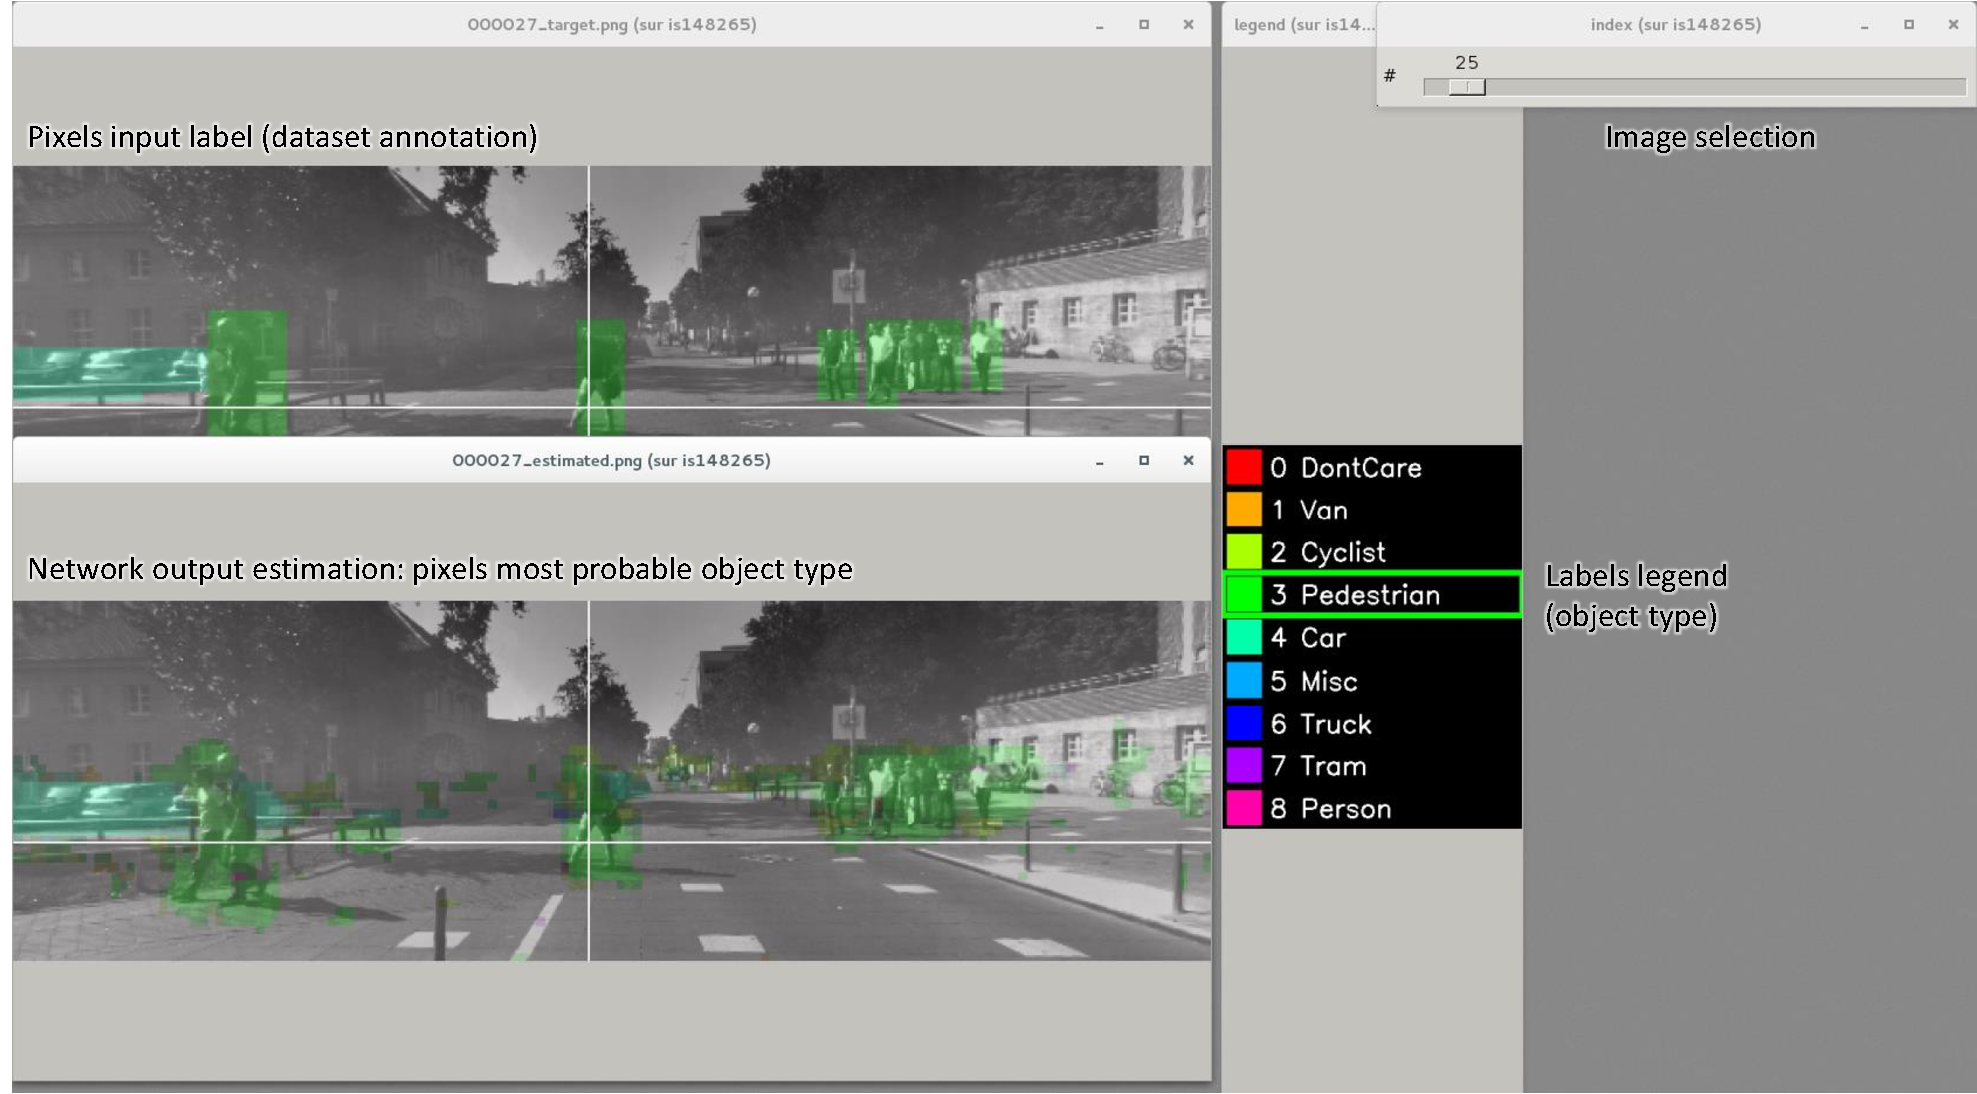
\includegraphics[width=1.0\linewidth]{figs/target_visu.pdf}
  \caption{Example of the target visualization helper tool.}
  \label{fig:targetvisu}
\end{figure}


\subsection{Transcoding a learned network in spike-coding}

N2D2 embeds an event-based simulator (historically known as 'Xnet') and allows
to transcode a whole DNN in a spike-coding version and evaluate the resulting
spiking neural network performances. In this tutorial, we will transcode the
LeNet network described in section \ref{sec:BuildingClassifierNN}.

\subsubsection{Render the network compatible with spike simulations}

The first step is to specify that we want to use
a transcode model (allowing both formal and spike simulation of the same
network), by changing the \lstinline!DefaultModel! to:

\begin{lstlisting}[language=ini]
DefaultModel=Transcode_CUDA
\end{lstlisting}

In order to perform spike simulations, the input of the network must be of type
\emph{Environment}, which is a derived class of
\emph{StimuliProvider} that adds spike coding support. In the INI model
file, it is therefore necessary to replace the \lstinline![sp]! section by an
\lstinline![env]! section and replace all references of \lstinline!sp! to
\lstinline!env!.

Note that these changes have at this point no impact at all on the formal coding
simulations. The beginning of the INI file should be:

\begin{lstlisting}[language=ini,escapechar=!]
DefaultModel=!\color{red}{Transcode\_CUDA}!

; Database
[database]
Type=MNIST_IDX_Database
Validation=0.2 ; Use 20% of the dataset for validation

; Environment
[!\color{red}{env}!]
SizeX=32
SizeY=32
BatchSize=128

[env.Transformation_1]
Type=RescaleTransformation
Width=[!\color{red}{env}!]SizeX
Height=[!\color{red}{env}!]SizeY

[conv1]
Input=!\color{red}{env}!
...
\end{lstlisting}

The dropout layer has no equivalence in spike-coding inference and must be
removed:

\begin{lstlisting}[language=ini,escapechar=!]
...
!\color{red}{\st{[fc1.drop]}}!
!\color{red}{\st{Input=fc1}}!
!\color{red}{\st{Type=Dropout}}!
!\color{red}{\st{NbOutputs=[fc1]NbOutputs}}!

[fc2]
Input=fc1!\color{red}{\st{.drop}}!
...
\end{lstlisting}

The softmax layer has no equivalence in spike-coding inference and must be
removed as well. The \emph{Target} must therefore be attached to
\lstinline![fc2]!:

\begin{lstlisting}[language=ini,escapechar=!]
...
!\color{red}{\st{[softmax]}}!
!\color{red}{\st{Input=fc2}}!
!\color{red}{\st{Type=Softmax}}!
!\color{red}{\st{NbOutputs=[fc2]NbOutputs}}!
!\color{red}{\st{WithLoss=1}}!

!\color{red}{\st{[softmax.Target]}}!

[fc2.Target]
...
\end{lstlisting}

The network is now compatible with spike-coding simulations. However, we did not
specify at this point how to translate the input stimuli data into spikes, nor
the spiking neuron parameters (threshold value, leak time constant...).

\subsubsection{Configure spike-coding parameters}

The first step is to configure how the input stimuli data must be coded into
spikes. To this end, we must attach a configuration section to the
\emph{Environment}. Here, we specify a periodic coding with random initial
jitter with a minimum period of 10 ns and a maximum period of 100 us:

\begin{lstlisting}[language=ini,escapechar=!]
[env]
...
ConfigSection=env.config

[env.config]
; Spike-based computing
StimulusType=JitteredPeriodic
PeriodMin=1,000,000 ; unit = fs
PeriodMeanMin=10,000,000 ; unit = fs
PeriodMeanMax=100,000,000,000 ; unit = fs
PeriodRelStdDev=0.0
\end{lstlisting}

The next step is to specify the neurons parameters, that will be common to all
layers and can therefore be specified in the \lstinline![common.config]!
section. In N2D2, the base spike-coding layers use a Leaky Integrate-and-Fire
(LIF) neuron model. By default, the leak time constant is zero, resulting
to simple Integrate-and-Fire (IF) neurons.

Here we simply specify that the neurons threshold must be the unity, that the
threshold is only positive and that there is no incoming synaptic delay:

\begin{lstlisting}[language=ini,escapechar=!]
[common.config]
...
; Spike-based computing
Threshold=1.0
BipolarThreshold=0
IncomingDelay=0
\end{lstlisting}

Finally, we can limit the number of spikes required for the computation of each
stimulus by adding a decision delta threshold at the output layer:

\begin{lstlisting}[language=ini,escapechar=!]
[fc2]
...
ConfigSection=common.config,fc2.config

[fc2.Target]

[fc2.config]
; Spike-based computing
TerminateDelta=4
BipolarThreshold=1
\end{lstlisting}

The complete INI model corresponding to this tutorial can be found in
\emph{models/LeNet\_Spike.ini}.

Here is a summary of the steps required to reproduce the whole experiment:

\begin{lstlisting}
./n2d2 "\$N2D2_MODELS/LeNet.ini" -learn 6000000 -log 100000
./n2d2 "\$N2D2_MODELS/LeNet_Spike.ini" -test
\end{lstlisting}

The final recognition rate reported at the end of the spike inference should be
almost identical to the formal coding network (around 99\% for the LeNet
network).

Various statistics are available at the end of the spike-coding simulation in
the \emph{stats\_spike} folder and the \emph{stats\_spike.log} file. Looking in
the \emph{stats\_spike.log} file, one can read the following line towards the
end of the file:

\begin{lstlisting}
Read events per virtual synapse per pattern (average): 0.654124
\end{lstlisting}

This line reports the average number of accumulation operations per synapse
per input stimulus in the network. If this number if below 1.0, it means that
the spiking version of the network is more efficient than its formal counterpart
in terms of total number of operations!


\clearpage

%\section{C++ Interface}
%
%\subsection{Databases}
%
%\subsubsection{Directory}
%
%Example:
%\begin{lstlisting}[style=c++]
%const double fracLearn = 0.5; // Fraction of stimuli used for the learning set
%const double fracValidation = 0.2; // Fraction of stimuli used for the validation set
%
%DIR_Database db;
%db.loadDir("path/to/images", 1, "", 1);
%db.partitionStimuliPerLabel(fracLearn, fracValidation, 1.0 - fracLearn - fracValidation, true);
%
%// Put the remaining stimuli in the testing set
%db.partitionStimuli(0.0, 0.0, 1.0);
%\end{lstlisting}
%
%\subsection{Environment}
%
%Example:
%\begin{lstlisting}[style=c++]
%Environment env(db,
%    /*SizeX=*/24,
%    /*SizeY=*/24,
%    /*BatchSize=*/12,
%    /*CompositeStimuli=*/false);
%env.addTransformation(PadCropTransformation(/*Width=*/24, /*Height=*/24));
%\end{lstlisting}


\bibliographystyle{abbrvnat}
\bibliography{biblio}

\fi

\end{document}
